% !TEX encoding = UTF-8 Unicode
% !TEX program = xelatex
% !BIB program = biber
% !TEX TS-program = xelatex
% !BIB TS-program = biber
%%
%%  本模板方式编译: XeLaTeX + biber
%%
%%  注意: 在改变编译方式前应先删除 *.toc 和 *.aux 文件
%%
\documentclass[12pt,openright]{book}

% 引入NKThesis包
\usepackage[emptydoublepage]{NKThesis}   % 中文
%\usepackage[emptydoublepage,English]{NKThesis} % 英文
\usepackage{amsmath}
\usepackage{newtxtext}
\usepackage{newtxmath}
\usepackage{bm}
\usepackage{algorithmic}
\usepackage{booktabs}
\usepackage{multirow}
\usepackage[linesnumbered,ruled]{algorithm2e}
\renewcommand{\algorithmcfname}{算法}
\renewcommand{\KwIn}{\textbf{输入:}}
\renewcommand{\KwOut}{\textbf{输出:}}
\newcommand{\tabincell}[2]{\begin{tabular}
{@{}#1@{}}#2\end{tabular}}
\usepackage{listings}
\usepackage{color}
% 其它包按需添加
% \usepackage{amsmath}
% \usepackage{cases}
% \usepackage{multirow}

% 参考文献
\addbibresource{nkthesis.bib}
% 图片文件夹
\graphicspath{{image/}}

\includeonly{
	./tex/abstract,
	./tex/introduction,
	./tex/method1,
	./tex/method2,
	./tex/method3,
	./tex/summary,
	./tex/references,
	./tex/acknowledgements,
	./tex/appendices,
	./tex/resume
}
\begin{document}
%  设置基本信息
%  注意:  逗号`,'是项目分隔符. 如果某一项的值出现逗号, 应放在花括号内, 如 {,}
%
\NKTsetup{
% 封面设置
论文题目(中文) = 基于数据驱动的软件维护关键技术研究,
副标题         = ,
论文题目(英文) = Research on the Data Driven Based Techniques for Software Maintenance,
论文作者       = 徐思涵,
学号           = 1120130140,
指导教师       = 许静~教授,
申请学位       = 博士,
培养单位       = 南开大学,
学科专业       = 软件工程,
研究方向       = 软件质量,
答辩委员会主席 = {},
评阅人 = {},
中图分类号     = ,
UDC            = ,
学校代码       = 10055,
论文完成时间   = 二〇一八年八月,
% 保密设置
密级           = 公开,	% 公开 | 限制 | 秘密 | 机密, 若为公开, 不填以下三项
非公开论文编号 = ,
保密期限       = ,
审批表编号     = ,
% 其他信息
批准日期       = ,
答辩日期       = ,
论文类别       = 博士, % 博士 | 学历硕士 | 专业学位硕士 | 同等学力硕士
院/系/所       = 计算机与控制工程学院,
联系电话       = 15102261750,
Email          = x.sihan@mail.nankai.edu.cn,
通讯地址(邮编) = 300350,
备注           = {}
}


% !TeX root = ../main.tex
% -*- coding: utf-8 -*-


\begin{zhaiyao}

	这里输入中文摘要。
\end{zhaiyao}




\begin{guanjianci}
	毕业论文;模板
\end{guanjianci}



\begin{abstract}


	This is the abstract.

\end{abstract}



\begin{keywords}
	Thesis; template
\end{keywords}

\tableofcontents

% !TeX root = ../main.tex
% -*- coding: utf-8 -*-
% !TeX root = ../main.tex
% -*- coding: utf-8 -*-

\chapter{绪论}
\label{chpt:introduction}
本章首先阐述本文的选题背景和意义,然后阐述论文的主要工作和创新点,最后介绍论文结构安排。

\section{研究背景与意义}
在软件生命周期中,随着外部环境的改变和用户需求的不断更新,软件开发人员必须不断修改软件系统以适应新的
需求。这种改变包括对软件错误的修复、新功能的添加和新的软件开发技术的应用等。然而,随着软件系统的不断
改变,代码结构变得越来越复杂,导致软件质量的逐渐下降。在软件演化过程中,为了保证软件质量,提高用户体
验,开发者有必要对软件系统进行维护。

软件维护是指在软件发布后,为了修复错误、改善设计、提升性能等提高软件质量的目的而进行的软件修改
~\cite{IEEE1219}。在现代软件系统中,软件维护是贯穿软件生命周期的软件活动,具有周期长、人员流动性强的
特点。软件维护人员需要花费大量的时间来理解和维护软件~\cite{Bansiya2002}。研究者发现,在整个软件生命周期
中,软件维护和演化的成本占总成本的80\%以上~\cite{guimaraes1983managing, coleman1994using}。由于软件
维护占据整个生命周期的大部分,因此不能快速和可靠地维护软件往往带来巨大的损失。

\subsection{软件维护的类型}

\begin{figure}
  \centering
  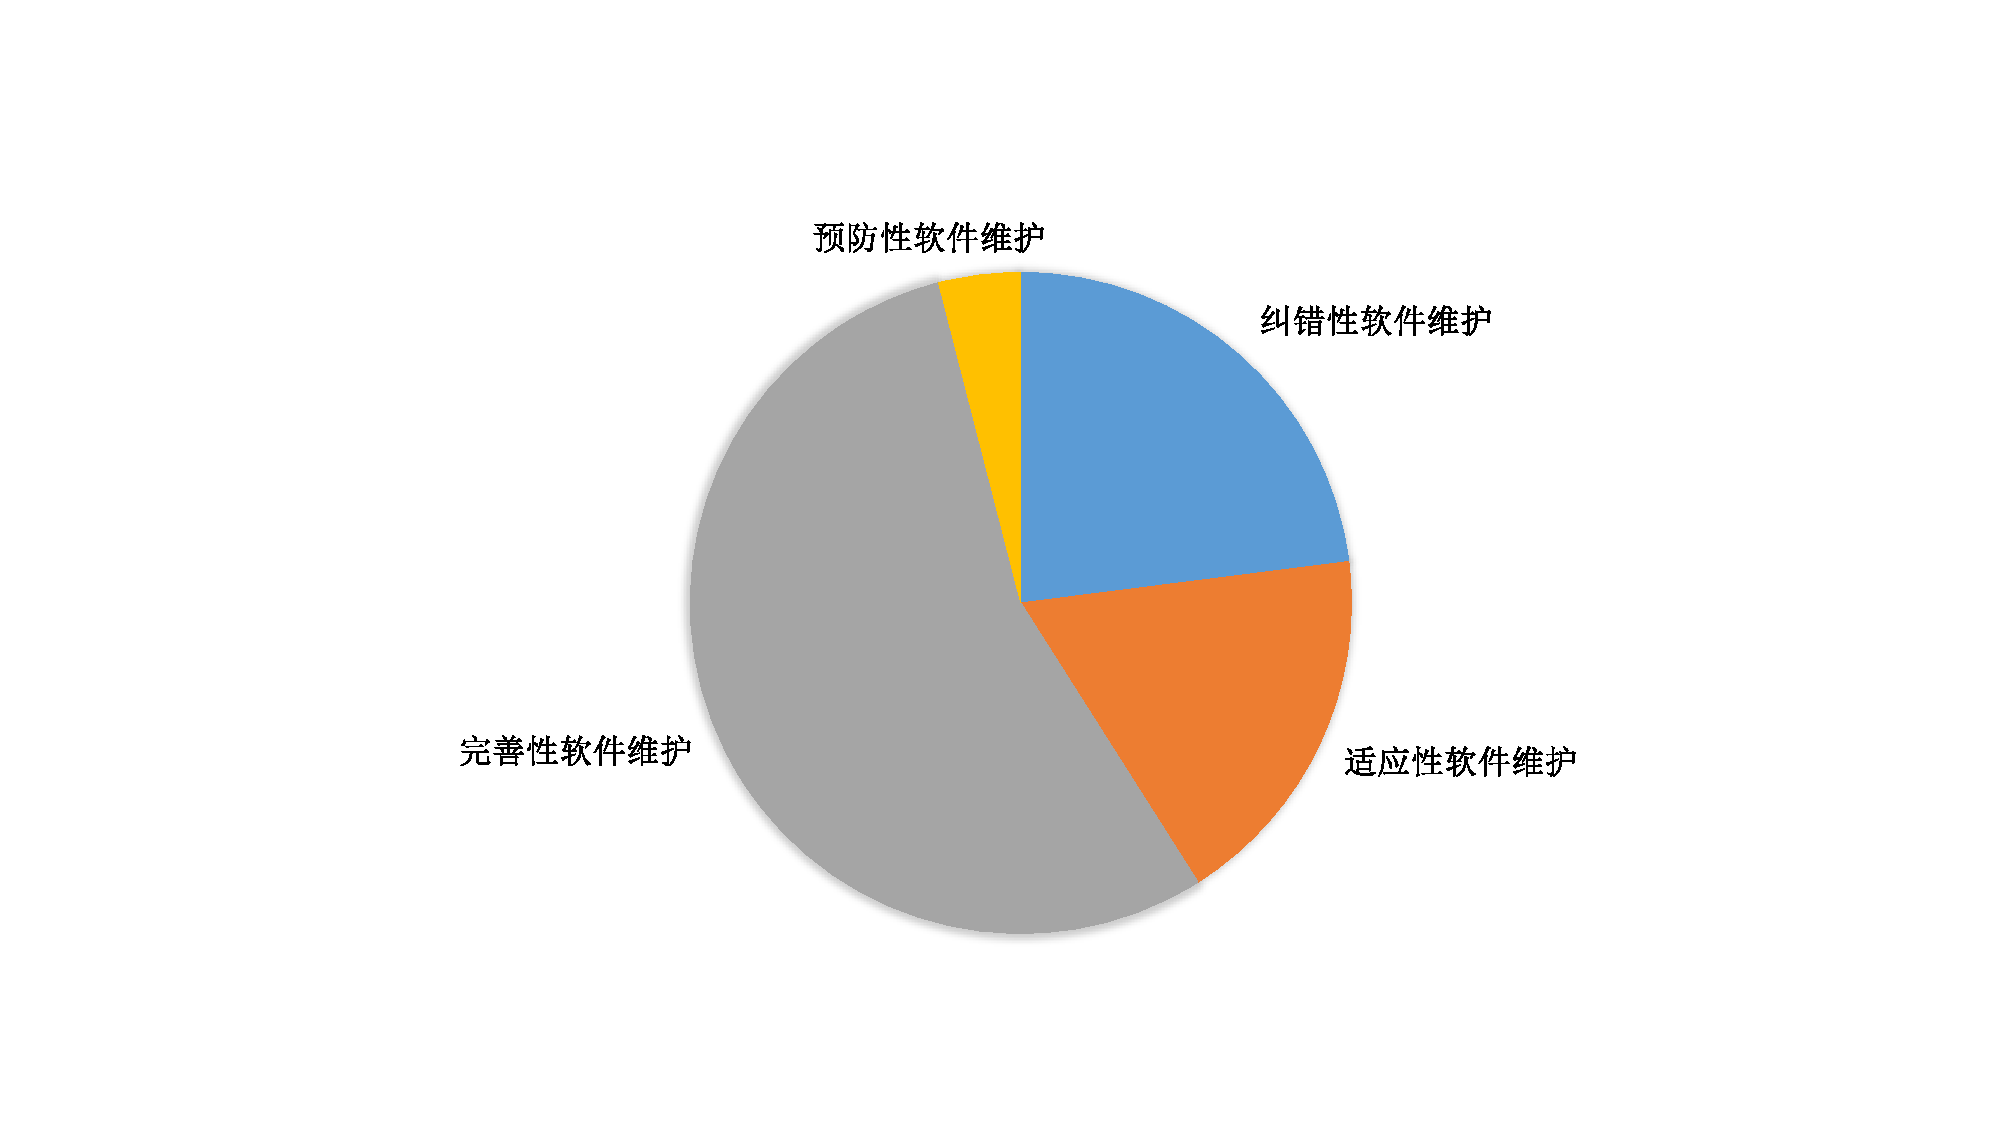
\includegraphics[width=0.6\linewidth]{maintenance.pdf}  
  \caption{\label{fig:maintenance}软件维护类型}
\end{figure}

如图~\ref{fig:maintenance}所示,软件维护可分为四种类型:纠错性软件维护、适应性软件维护、完善性软件维
护和预防性软件维护~\cite{lientz1978characteristics}。

\begin{itemize}
  \item 纠错性软件维护是提高软件可靠性的重要手段,指的是纠正在软件开发过程中未被发现的,实际应用中出
现软件行为与预期不相同的错误。由于软件开发过程中很难做到发现所有潜在的错误,因此在软件系统的实际应用
中,可能会触发软件错误,导致系统不能正常运行,可能给经济和社会带来巨大的损失。根据美国的标准与技术研
究报告,软件缺陷为美国带来每年高达600亿美元的损失,而即使发现软件缺陷则会为美国每年节约超220亿美元
~\cite{strate2013literature}。纠错性软件维护通常是在软件发生缺陷时进行的对软件缺陷的定位、诊断和修
复。
  \item 完善性软件维护则是关系到软件系统质量的重要方面,包括改进程序设计、提升软件运行的效率和性能
等。在软件的使用过程中,随着外部环境的不断变化和用户需求的不断提升,用户对系统的功能和性能要求也逐步
提高。然而,由于缺陷修复和新功能的添加,程序变得越来越复杂,导致软件质量逐渐降低。完善性软件维护通过
改进软件设计、提高运行效率等手段来提高软质量,在延长软件寿命的同时降低软件维护成本。
  \item 适应性维护通常是为了让软件适应技术和外部环境的变化而进行的。一方面,随着软件开发技术的发展和
操作系统版本的更迭,软件维护人员需要不断改进软件从而适应新的技术环境;另一方面,硬件环境的更新带来系
统性能和效率的大幅度提升,这就要求软件维护人员有计划性地修改软件系统,从而适应新的硬件环境。
  \item 预防性软件维护是为了适应未来软件的环境变化,将被动转化为主动而添加的新功能。对软件系统的维护
工作并不一定只能在软件系统出了错误或是用户提出需求才能执行,合理的预防性的软件维护可以将软件维护的成
本降低,提高用户的使用体验。对正在使用中的软件系统,预防性软件维护考虑到将来可能发生的修改,对软件系
统实施有计划性的修改,从而使其容易适应环境和需求的改变,不易被淘汰。
\end{itemize}

由图~\ref{fig:maintenance}中可以看出,纠错性和完善性软件维护是最主要的两种软件维护手段,占软件维护总
量约75\%。纠错性软件维护是保证软件正确性的重要手段,是完善性软件维护的基础;同时,完善性软件维护通过
改进软件设计、提高软件质量的方式,让代码更易读,提高缺陷定位和错误修复的效率。


\subsection{基于数据驱动的软件维护}
由于当代软件系统具备代码规模大、迭代周期短等特点,人工软件维护变得越来越困难。一方面,软件维护依赖于程序
员对软件系统细致的理解。然而,随着软件系统规模的扩大,代码的复杂度也越来越高,即便是经验丰富的软件维
护人员也很难完全掌握整个软件系统,导致人工进行软件维护变得越来越困难,且其效果也容易受到个体思维的影
响。另一方面,软件维护通常具备周期长、人员流动性大、工作枯燥繁复等特点,人工进行软件维护
不但需要大量的人力资源,其效率也会随着软件复杂性的提升而不断降低,导致软件维护的时间和人力成本较高,
很难满足当代软件系统快速迭代的要求。

自动化的软件维护可以解决人工维护的效率低、易受个体思维影响的缺点,因此,很多研究者致力于提出各种自动
化、半自动化技术来提高软件维护的效率和性能。例如,在纠错性软件维护方面,研究者们提出用自动化测试技术
来代替传统的人工测试,从而解决人工测试中的遗漏、思维惯性等问题,使测试更快、更可靠、更便宜。在完善性
软件维护方面,大多数集成开发环境,如Eclipse和IntelliJ IDEA等,提供了软件重构的支持工具作为插件。 当
开发人员需要重构时,首先选择待重构代码,然后选定软件重构类型以及必要的输入(如函数重命名操作中的新函
数名),重构工具可以替代软件维护人员完成剩下的工作。这样的工具为自动和半自动化软件重构提供了基础,是
软件重构被广泛应用的重要因素~\cite{griswold1993automated,tip2003refactoring,mens2005formalizing}。

然而,由于软件维护的复杂性,研究者很难制定一套完整而严密的规则来解决软件维护中的难题,因此当前的软件
维护工作很难被完全自动化的技术所完成。例如,虽然自动化测试技术可以大量的减少枯燥重复的工作,提高软件
测试的效率,然而对测试结果的判定依赖软件维护人员,自动化判断测试用例的预期表现仍然是尚待解决的难题。
同样,基于集成环境的软件重构工具通过开发工具来为特定类型的手动重构操作提供技术支持
~\cite{fowler1999refactoring, murphy2012we}。虽然很多编辑器和集成开发环境集成了这类重构支持工具,其
作用仅仅是替软件维护人员执行指定的重构操作,仍然依赖于软件维护人员来识别软件重构机会和选择软件重构操
作。因此,手动重构的过程较为复杂和乏味,软件维护人员需要花费大量的时间和精力指定需要被执行的软件重构
操作。

数据挖掘对于这种存在内部规律但却很难通过人为制定完整规则来解决的难题提供了一种新的解决思路,即挖掘数
据中潜在的规律作为解决方案。成熟的开源社区和版本控制工具(如CVS、Git、SVN等)为研究者们提供了大量的
可研究数据,包括软件系统的版本、规模、复杂度、修改等。从数据的角度来理解软件系统,将软件维护问题转换
为数据挖掘问题,既避免了对软件维护人员经验的依赖性,又提高了维护效率,减少了时间和人力的成本,因此成
为了近几年软件工程的研究热点。随着信息化的发展,大量的软件代码可以被研究使用,与软件相关数据的价值逐
渐被研究者认可。机器学习和数据挖掘算法被广泛应用于缺陷预测
~\cite{menzies2007data,drown2009evolutionary,khoshgoftaar2010attribute}、缺陷定位
~\cite{malcov2013,nnfault2013}、补丁生成~\cite{martinez2015mining, long2016automatic}等方面。本文主
要针对纠错性软件维护和完善性软件维护中的关键技术,使用数据挖掘提供解决方案,为软件维护人员减少时间和
人力的成本,从而适应当代软件系统提高可靠性和实现快速迭代的需求。

\iffalse
在程序修复方面,Martinez等人~\cite{martinez2015mining}通过挖掘软件仓库中的修复数据,为抽象语法树的修
改和错误修复之间的关系建模,预测修复错误的概率。Long~\cite{long2016automatic}等提出通过挖掘成功修复
错误的补丁,为每个成功的补丁提取了面向修改和数值的特征,前者表示程序修改和周围代码的关系,后者表示修
改前后变量数值的改变;最后通过最大似然来预测补丁可能能够成功修复错误的概率。
\fi

\section{研究内容与创新点}
本文研究内容主要针对软件维护中两种主要的软件维护类型,即纠错性和完善性软件维护。纠错性软件维护是保证软
件正确性的重要手段,然而在纠错性维护后,虽然软件系统的正确性得以保障,但对软件系统的修改可能会导致软
件系统设计的偏离,使得软件质量降低。为了提高软件质量,通常需要后续进行完善性软件维护。

首先,为了保证软件系统的正确性,以测试用例执行作为数据基础,提出了基于Relief特征选择和分支覆盖特征谱
的缺陷定位技术。然后,为了完善软件系统设计,以开源软件仓库中的重构实例作为数据基础,针对软件系统维护
中最常见的两种软件重构操作--函数抽取和重命名重构,提出了基于数据挖掘的重构机会推荐方法。本文研宄内容
如下:

(1)基于特征选择的缺陷定位

为了提高纠错性软件维护的效率,本文研究了基于覆盖分析的缺陷定位方法(CBFL),其核心思想是被失效用
例执行越多、成功用例执行越少的代码可疑度越高~\cite{jones2005empirical}。其方法通常是收集测试用例在执
行过程中的语句、谓词或分支等覆盖信息并统计执行结果,然后根据特定的可疑度计算公式来计算代码的可疑度。
该方法用较低的计算成本计算代码的可疑度,并按照可疑度大小由高至低推荐给软件维护人员。然而,软件系统中
可能存在不止一个错误,导致测试用例失效原因也可能不止一个。基于覆盖率的缺陷定位方法,忽略了不同软件错
误之间的相互影响,因此可能导致准确性降低。

Kira等人~\cite{kira1992feature}最早提出利用相关统计量度量特征的重要性,该方法为每个测试用例分别寻找
距离最近的同类和异类,距离同类越近、距离异类越远的特征被认为越能够区分不同类别的样本,因此对样本的类
别越重要。本文引入相关统计量的概念,通过将测试用例执行的覆盖信息作为特征,测试用例执行结果作为标签,
将原问题转化为数据挖掘问题,从而推测特征(代码)对执行结果的重要性。基于由相同软件错误引发的失效用例
其覆盖信息可能相似的思想,本文通过为每个测试用例选择距离最近的同类/异类样本,在很大程度上避免了由不
同错误引发的失效样例,从而提高可疑度计算的准确性。

(2)基于梯度提升决策树的函数抽取重构机会推荐

为了提高完善性软件维护的效率,本文面向最常见的软件重构操作--函数抽取重构操作,提出基于梯度上升决策树
的重构机会推荐。当前基于软件度量和代码切片的重构机会推荐方法往往依据特定的软件度量进行排序推荐,违背
了软件重构原因的多样性和复杂性~\cite{silva2016we}。为了探究函数抽取重构的根本原因,本文通过观察开源
软件重构实例,将函数抽取重构作为训练数据,从模型的角度探讨函数抽取重构的原因,并为软件维护人员推荐重
构操作。

在训练阶段,本文收集大量的开源函数抽取重构实例作为正样本,并随机生成等比例的负样本作为训练数据。本文
提出基于软件质量概念的特征提取算法,融合了凝聚度、耦合度、复杂度三个重要概念,并考虑了多种程序元素,
如变量、类型、函数调用、包等,使用梯度提升决策树和逻辑斯特回归的融合模型进行训练。在预测阶段,首先为
给定函数体生成所有合法的候选函数抽取重构操作,然后使用该融合模型进行训练,得到每个候选操作被分为正类
的概率,并根据概率由高至低进行排序,推荐给软件维护人员。

(3)基于层次注意力网络的函数名推荐

在完善性软件维护阶段,为了提高软件系统的易读性和可维护性,本文面向函数重命名软件重构类型提出了基于注
意力机制的推荐模型。由于软件维护的周期长、人员流动性大的特点,易读性高的软件系统其维护成本较低。好的
函数名通常具备功能描述性强的特点,因此可以提高软件维护人员错误修复、功能添加的效率。研究表明,函数抽
取和函数重命名是最常用的两种软件重构操作。为了研究好的函数名和函数体之间的关系,本文提出使用层次注意
力网络模型为给定代码片段预测其函数名。

本文的训练数据来自于GitHub上广受欢迎的开源软件,因其在多数情况下被认为具有较强的代码规范性。每个函数
的``函数名-函数体''对被视为一个训练样本。将分词后的函数体表示为一个词序列,将每个基本块视为一个功能
子单元,根据``多个基本块子功能组成一个函数,多个词组成一个基本块''的层次结构,提出使用层次注意力网络
模型来拟合函数体与函数名之间的关系。在预测阶段,本文首先将给定函数体表示为上述层次结构,然后使用层次
注意力网络进行预测,最后使用集束搜索生成具有概率的函数名,并按照概率的由高至低推荐用户。

\section{论文结构安排}
\begin{figure}[htp]
  \centering
  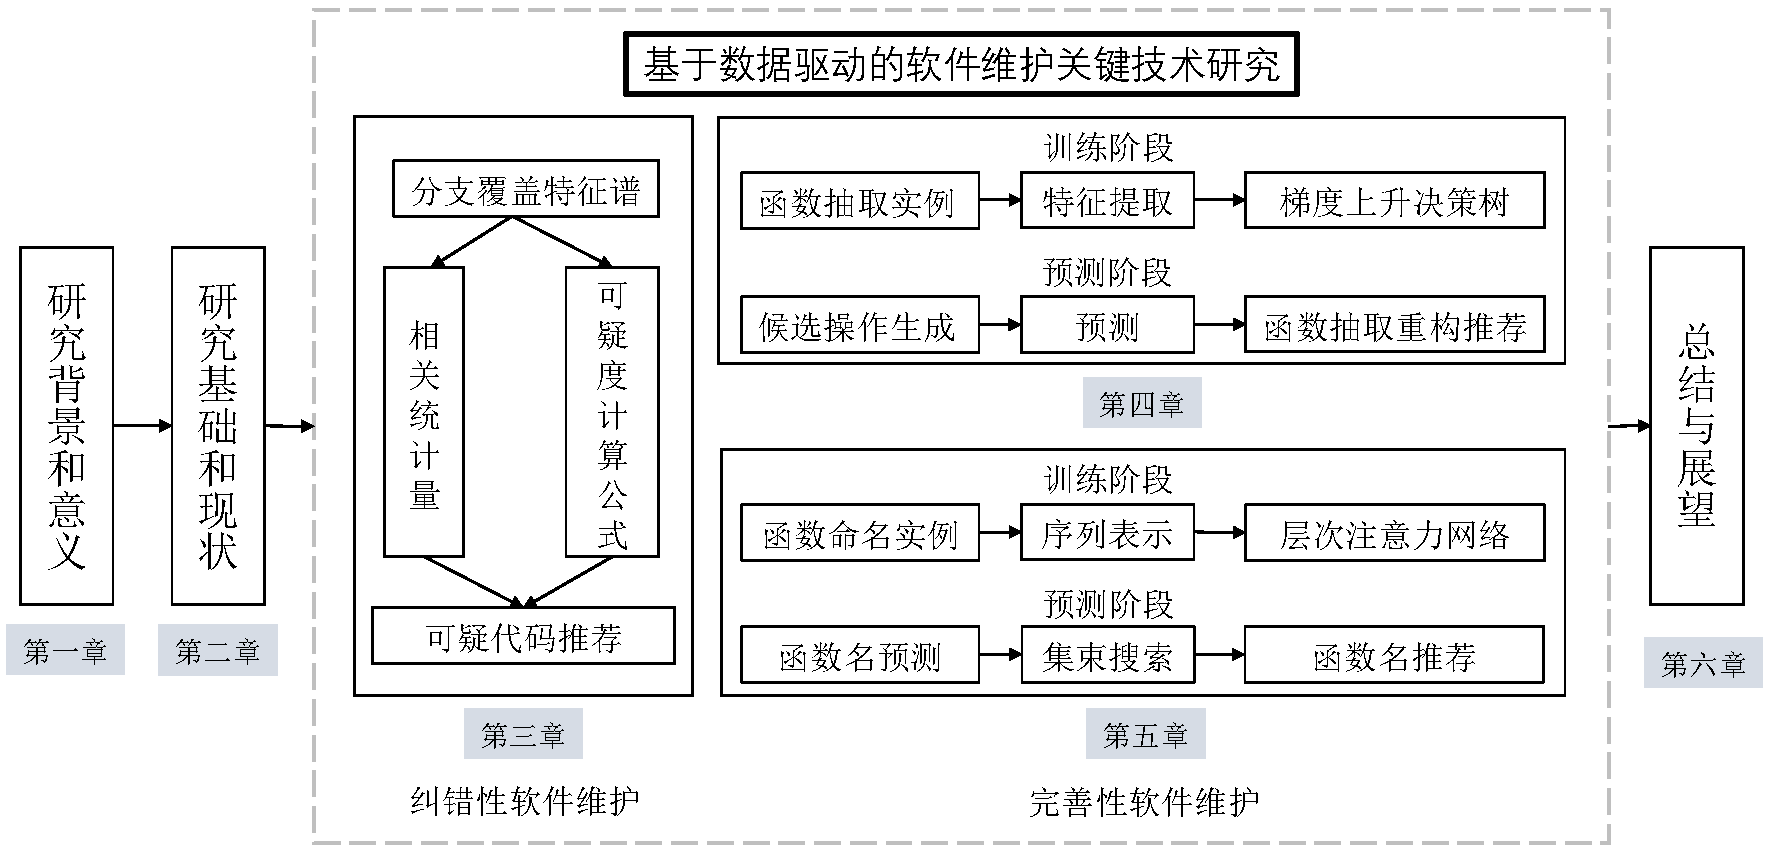
\includegraphics[width=1.0\linewidth]{org.pdf}
  \caption{论文组织结构}
  \label{fig:org}
\end{figure}

如图~\ref{fig:org}所示,本文共分为六章。首先,第一章介绍了本文研究的背景和意义,以及本文的主要研究内容和创新点。后续章节的内容如下:  

第二章介绍本文的研宄基础与现状。本文针对的两种主要的软件维护类型,即纠错性维护和完善性维
护,进行研究。本文首先介绍了缺陷定位相关研究现状;然后介绍了软件重构的相关基础,包括软件质量和代码坏味的关系、软件重构操概述和软件重构推荐方法的研究现状。

第三章提出了基于Relief特征选择的缺陷定位方法。首先介绍了基于分支覆盖特征谱的缺陷定位方法的一般流程,然后介绍了相关统计量的概念和方法。接着使用相关统计量来推测代码覆盖信息对测试用例执行结果的重要性,将其作为可疑度的辅助计算方法,与Ochiai可疑度相结合。最后将代码按照可疑度排序,由高至低推荐给用户。

第四章提出了基于梯度上升决策树的函数抽取重构机会推荐方法。首先介绍了使用梯度上升决策树进行二分类的原理,然后介绍了本文的梯度上升决策树分类和逻辑斯特回归融合模型,接着介绍函数抽取重构实例数据收集方法以及特征提取算法。在预测阶段,介绍了基于代码块的候选重构操作生成,并基于预测结果排序。最后介绍了本文的实验部分,包括实验数据集和评价指标,以及在不同模型和数据集上的实验结果。

第五章提出了基于层次注意力网络的函数名推荐方法。首先介绍了层次结构的代码片段表示方法,然后介绍了层次注意力网络模型和集束搜索(Beam Search)在模型中的应用。最后描述了本文的实验部分,包括实验数据集和评价标准,以及与其它经典的函数命名方法的对比实验结果。

第六章对本文进行总结,并展望接下来的研究方向。

\chapter{研究基础和现状}
本章首先介绍了纠错性软件维护的相关工作,包括缺陷定位和缺陷预测等;然后介绍了完善性软件维护的研究基
础,包括软件质量和代码坏味的关系、软件重构操概述和软件重构推荐方法等。
\section{纠错性软件维护}
纠错性软件维护是保证软件系统正确性的重要手段,本节主要介绍缺陷定位的相关研究工作,并简单介绍其它纠错
性软件维护,如缺陷预测。
\subsection{缺陷定位}
软件缺陷是导致软件系统行为与预期不一致的主要原因。为了帮助软件维护人员迅速消除缺陷,首要任务就是找到
软件缺陷在源代码中的位置,即缺陷定位。当软件失效时,缺陷定位是保障软件系统正确性的重要手段。缺陷定位
方法主要有覆盖分析、程序切片、依赖分析、程序不变量等。

(1)覆盖分析法

覆盖分析指的是根据程序执行过程中的覆盖统计信息,按照特定的可疑度计
算公式计算代码可疑度,并按照可疑度高低排序推荐的过程。由于覆盖分析的计算成本低,准确性较高,因此得到
了广泛的关注。其核心思想是,被失效用例执行越多、成功用例执行越少的代码可疑度越高
~\cite{jones2005empirical}。

基于覆盖分析的缺陷定位,其一般过程是首先执行测试用例,收集测试用例对程序元素(如语句、谓词或分支等)
的覆盖信息并统计执行结果(失效或成功),然后使用特定的可疑度计算公式计算可疑度,并将程序元素按照可疑
度由高至低排序,推荐给软件维护人员进行缺陷定位。基于覆盖分析的缺陷定位,其流程大多相似,主要区别在于
可疑度计算公式。表~\ref{fig:susp}中展示了较为经典的六种可疑度计算公式,为了便于理解,所有公式都沿用
Tarantula中的变量定义。Ochiai公式最先在生物学中作为基因相似度的度量公式被提出,Abreu等人
~\cite{abreu2007accuracy}将其运用到可疑度计算中,并得到不错的表现。同时,受聚类分析的启发,他们提出
使用相似度系数Jaccard来度量程序代码的可疑度~\cite{abreu2007accuracy}。Wong等人
~\cite{wong2008crosstab}提出基于交叉表的方法计算代码可疑度,认为覆盖某个程序元素的测试用例,其被失效
执行次数越多,成功执行次数越少,则该程序元素越可能包含缺陷。该方法通过计算相同程序元素被失效执行和成
功执行的相差次数来计算可疑度。Kulczynski公式最早出现在生物学中~\cite{willett2003similarity},Wong等
人~\cite{wong2014dstar}将其扩充后用来计算代码可疑度,其借助失效用例的相似性来进行缺陷定位,在实验数
据集上得到了较高的准确度。Naish等人~\cite{naish2011model}对比了36种基于覆盖分析的缺陷定位方法,根据
实验结果将这些覆盖分析法的可疑度计算公式分为组,每组的计算公式互相等价,并得到Optimal排序方法较其它
方法表现更好的结论。

\begin{center}
\tablecaption{经典可疑度计算公式}\label{fig:susp}
\begin{tabular}{|c|c|}
\hline
覆盖分析法 & 可疑度计算公式 \\ \hline
Tarantula & $\frac{\frac{a_{11}}{a_{11}+a_{01}}}{\frac{a_{11}}{a_{11}+a_{01}}+\frac{a_{10}}{a_{10}+a_{00}}}$\\ 
Jaccard & $susp = \frac{a_{11}}{a_{11}+a_{01}+a_{10}}$\\ 
Ochiai & $susp = \frac{a_{11}}{\sqrt{(a_{11}+a_{01})\times(a_{11}+a_{10})}}$\\
Ochiai2 & $susp = \frac{a_{11}a_{10}}{\sqrt{(a_{11}+a_{10})\times (a_{00}+a_{10})\times (a_{11}+a_{01})\times (a_{01}+a_{00})}}$\\ 
Wong & $susp = a_{11}-a_{10}$\\
DStar & $susp = \frac{a_{11}^{star}}{a_{10}+a_{01}}$\\ 
Naish2 & $susp = a_{11}-\frac{a_{10}}{a_{10}+a_{00}+1}$ \\
Optimal & $susp = \begin{cases}
  -1, & \text{ if } a_{01}>0 \\ 
  a_{00}, & \text{ elsewise }  
  \end{cases}$\\ \hline
\end{tabular}
\end{center}





(2)程序切片法


(3)依赖分析法

(4)其它方法

在缺陷定位方面,张云乾等人~\cite{malcov2013}认为缺陷定位技术的准确性和错误类型有关,因此提出使用马尔
科夫模型预测错误类型,然后选用有针对性的缺陷定位技术进行缺陷定位。何加浪和张宏~\cite{nnfault2013}通
过建立神经网络学习错误和输入之间的关系,通过计算程序中每个位置对错误的支持度来进行多缺陷定位。

\subsection{缺陷预测}

在缺陷预测方面,Menzies等人~\cite{menzies2007data}使用朴素贝叶斯模型进行缺陷预测,并提出在预处理阶
段,使用对数操作可以提升缺陷预测能力。Drown等人~\cite{drown2009evolutionary}提出了基于遗传算法的缺陷
预测模型,利用遗传算法中的指标优化采样过程。Khoshgoftaar等人~\cite{khoshgoftaar2010attribute}提出结
合特征选择和采样的模型来进行缺陷预测。
\section{完善性软件维护}

\subsection{代码坏味}
代码坏味是软件系统中出现``坏代码''的信号,通常被研究者认为软件系统需要进行重构的信号。Fowler等人提出
了22种软件结构作为代码坏味的表现,并认为这些代码坏味可以帮助软件维护人员决定软件是否需要被重构
~\cite{fowler1999refactoring}。同时,Fowler等人提出了72代码重构操作,在保持程序外在行为的一致性的同
时,改进程序内部的设计结构~\cite{fowler1999refactoring}。在表~\ref{fig:badsmell}中我们列举了其中十种
经典的代码坏味,以及可能解决这些代码坏味的软件重构操作。

\begin{center}
\tablecaption{十种经典代码坏味}\label{fig:badsmell}
\begin{tabular}{|l|l|l|l|}
\hline
序号 & 代码坏味 & 软件重构操作 & 重构目标\\ \hline
1 & 代码重复 & 函数提炼、函数上移、类提炼 & 提取公共代码\\ \hline
2 & 函数过长 & 函数提炼 & 拆分函数\\ \hline
3 & 类过大 & 类提炼 & 拆分类\\ \hline
4 & 参数过多 & 引入参数对象、函数替代参数 & 减少参数\\ \hline
5 & 发散式变化& 类提炼 & 将全部变化提取到新类\\ \hline
6 & 霰弹式改动& 函数移动、类内联 & 将全部修改合并为同类\\ \hline
7 & 依恋情节& 函数提炼、函数移动 & 移动依恋代码\\ \hline
8 & 数据泥团& 类提炼、引入参数对象 & 简化数据\\ \hline
9 & 基本类型偏执& 对象替换数据 & 简化类型 \\ \hline
10 & Switch语句 & 函数提炼、函数移动 & 减少Switch语句\\ \hline
\end{tabular}
\end{center}

值得注意的是,每一种代码坏味可以被一种或多种软件重构操作所解决。如表~\ref{fig:badsmell}中的代码重
复,在很多情况下可以通过函数提炼(Extract Method)提取重复的代码结构作为一个新的函数被调用;当重复代
码出现在两个兄弟子类时,可以分别在这两个子类中进行函数提炼,然后将该函数上移(Pull Up Method)到这两
个子类的父类中;当重复代码出现在两个不相干的类中时,可以将重复代码提取为一个新类(Extract Class),
在原来的两个类中调用这个新类。因此我们可以看出,即使针对同一代码坏味,在不同的情况下软件维护人员需要
选择不同的重构操作,甚至是一系列重构操作的叠加。

代码坏味不完全是相互独立的,有一些代码坏味是相关联的,因此可以被相同的软件重构操作所解决。例如代码重
复可能会导致函数过长或者类过大,此时如果使用函数提炼或类提炼,既解决了代码重复的问题,同时也解决了函
数过长或者类过大的问题。同样,依恋情节通常发生在某个函数对某个类的兴趣远高于其所在的类,此时会导致该
函数频繁的访问该类,可能导致函数过长、类过大、参数过多以及发散式变化(容易受到该类的影响)等代码坏
味。通过将部分依恋代码提炼成新的函数,并移动到其频繁访问的类(Move Method),可以让大部分问题得到改
善。

有一些代码坏味是互斥的,因此它们所对应的软件重构操作也是互为逆向操作。如表~\ref{fig:badsmell}中的类
过大和霰弹式改动是两个互斥的代码坏味。当我们用类提炼将大类拆分成多个小类时,虽然每个类的规模变小,但
容易引发霰弹式改动的问题,即原来在同一个大类中的多个小类由于彼此依赖,导致当改动其中一个小问题时,引
发一系列发散的改动,造成软件维护的不便;反之,当我们用类内联(Inline Class)将某个修改所涉及到的修改
都集合到同一个大类中时,虽然解决了霰弹式改动的代码坏味,但此时容易引起类过大的问题。这样逆向的软件重
构操作还有函数提炼和函数内联(Inline Method)、函数上移和函数下移(Pull Down Method)等。因此,如何
针对软件系统选取合适的软件重构操作是软件维护人员需要解决的问题。

虽然代码坏味是软件重构的重要信号,但是软件重构的动机却不完全是为了解决代码坏味。Silva等人
~\cite{silva2016we}调查研究了软件开发人员进行软件重构的动机。调查发现,软件重构主要发生在需求发生改变
的时候,如增加新特性或是修复软件错误时,因此软件重构的动机通常与提高软件的易读性、可重用性、易测性等
相关,而不仅仅是针对特定代码坏味的修复。以最常用的软件重构操作--函数提炼为例,调查显示,软件维护人员
进行函数提炼重构的原因较为复杂,包括代码重用、函数分解、加速扩展、重命名内部函数等11种主要原因。其
中,只有函数分解与代码坏味有关,其通常被认为是决代码坏味``函数过长''的方法。由于人工识别软件重构机会
并选择软件重构操作的成本较高,且软件重构的动机具有复杂性和多样性,研究者们提出了很多软件重构推荐技术
来解决该问题,关于软件重构推荐的研究引起了广泛关注。

\subsection{软件重构原理概述}

软件重构提高软件质量,降低软件维护成本的重要手段之一。重构这个术语最早由William
Opdyke~\cite{opdyke1992refactoring}在其博士论文中提出的。软件重构技术旨在在不改变软件整体功能的前提
下,改进软件的设计结构,使得新的设计结构提高代码的可维护性,从而提高软件的质量
~\cite{fowler1999refactoring}。因此,软件重构通常只改变软件的外观,比如在传统的结构化设计上以改进其
结构。软件重构不涉及修改软件的语义和功能,而是通过更好的观察软件系统,从而提出对软件系统设计各方面的
改进~\cite{chikofsky1990reverse}。

\begin{figure}
  \centering
  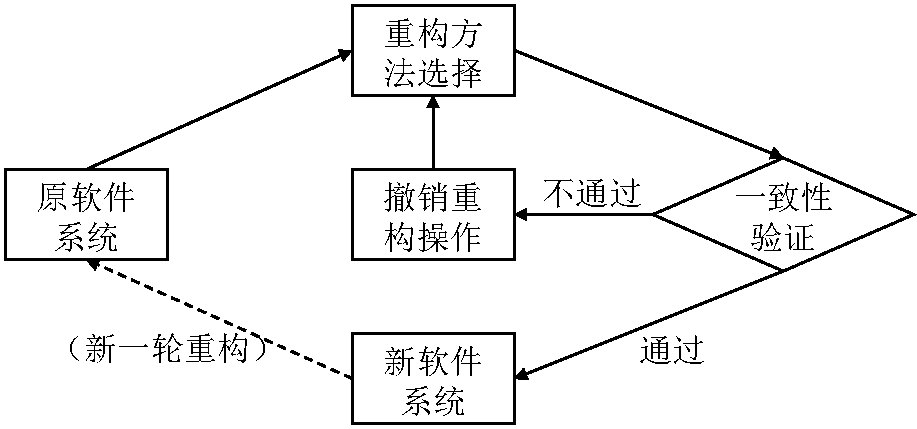
\includegraphics[height=45mm, width=90mm]{refactory.pdf}  
  \caption{\label{fig:refactory}软件重构一般过程}
\end{figure}

软件重构的一般是通过迭代转换的方式对软件系统进行转换。图~\ref{fig:refactory}描述了这样的转换过程。针
对原软件系统,每一轮迭代是对软件的一次小规模转换,针对特定代码选择某种重构方法,在实施软件重构操作后
测试其正确性,即测试软件的语义和功能是否与原来的保持一致。若测试通过,则本轮重构完成,软件维护人员可
在新的软件系统上进行新一轮重构。在任何时间一旦测试不通过,则最后一次程序转换撤销,需要重新选择重构方
法,换一种方式进行重构。通过很多轮这样的小规模程序转换,软件重构的过程和细节可以完全被软件维护人员所
掌控,并达到其所预想的效果。这样的迭代过程要求测试过程十分迅速,否则软件维护人员将不得不花费大量的时
间等待测试完成。因此,很多极限编程和其它敏捷软件开发的使用者将这种迭代过程作为软件开发周期的一个重要
组成部分。除此以外,为了减少一致性验证所带来的测试时间成本,部分学者提出使用先置性条件过滤,使得满足
条件的软件重构能保持语义和功能的一致性,从而减少不必要的测试成本。

软件重构是影响软件完善性维护的重要方面。在软件生命周期中,新的需求被不断添加,使得代码的复杂度越来越
高,代码结构逐渐偏离原来的设计,从而导致了扩展软件的难度越来越大。软件重构增加了程序设计的灵活性,通
过改进软件设计,使得软件具备高凝聚、低耦合和复杂度低等特点,将复杂代码变简单,从而提高代码的可扩展
性,降低软件的维护成本。完善性软件维护的时机通常与软件系统质量有关。软件质量下降时,软件系统发出需要
重构的信号。最常见的情况是当软件维护人员修补错误或添加新功能时,首先要需要做的就是理解代码。当代码可
读性强,容易被理解时,修复软件错误和添加新功能的效率更高。相反,当代码复杂度高、不容易被理解时,代码
的质量下降,可维护性也随之降低,此时通常需要对软件进行重构。完善性软件维护可以加速当前和未来对代码的
理解,从而提高软件维护效率。

\subsection{软件重构检测}
软件重构检测通过检测相同软件系统不同版本之间发生的软件重构操作,帮助软件维护人员熟悉代码改变的意图,
更好地了解软件的演化过程。Robbes等人~\cite{robbes2008spyware}开发了一个工具集Spyware来监视集成开发环
境。该工具将软件开发人员对代码的修改表示为基于语义的修改序列,并将这些重要的修改存储起来,开发者可以
通过观察和重放这些修改来观测到软件重构的发生。

大多数研究者主要通过比较两个软件版本中代码的相似度来检测软件重构。Demeyer等人
~\cite{demeyer2000finding}首次提出通过比较相同软件系统的不同版本来检测软件重构的方法,该方法通过比较
软件度量,如代码行数(LOC)和函数调用个数等,检测是否存在软件重构。Malpohl等人
~\cite{malpohl2003renaming}通过使用diff命令来比较两个函数的相似度,从而推测出函数重命名的重构操作。
Antoniol等人~\cite{antoniol2004automatic}提出了基于向量空间的信息检索方法检测代码重构。Xing等人
~\cite{xing2005umldiff}基于命名和结构相似度,自上之下比较了包、类、借口等程序元素。同样基于相似度原
理,部分研究者将克隆检测器应用于软件重构检测中,将不同版本的函数相对应,从而检测出函数提炼和函数移动
等软件重构操作~\cite{van2003reconstruction,kim2005functions}。Weißgerber等人
~\cite{weissgerber2006identifying}提出将软件仓库通过预处理存储进关系型数据库中,然后将每次提交的代码
修改作为事务创建,从中分析出增加、修改或删除的类、字段和函数,从而得到可能的软件重构操作,最后使用克
隆检测将这些操作排序。

由于软件重构的本质是保持软件的语义不变,改变其内部结构,因此有研究者提出使用基于语义分析的方法检测软
件重构。Dig等人~\cite{dig2006automated}开发了基于Eclipse的插件,其首先通过语义分析函数调用、类型使
用、实例化等关系,然后使用一种迭代的方法自顶而下的检测重构。Fluri等人~\cite{fluri2007change}比较了两
个版本的抽象语法树,计算了基于抽象语法树的修改操作,并将其映射到抽象语法树级别的代码修改上。这种方法
的优点在于识别了语法树级别的原子改变,但是由于其停留在原子改变,而未将多处改变抽象化分析,导致其很难
检测出更抽象级别的软件重构。

由于基于相似度比较的软件重构检测方法,其侧重点在于不同版本的软件系统的比较,导致其所能检测出的软件重
构的类型有限,大多为函数移动、函数重命名等简单的重构类型;而复杂重构类型往往涉及多处修改,因此很难被
基于相似度比较的方法检测到。Taneja等人~\cite{taneja2007automated}开发了一种工具RefacLib,通过句法分
析来检测代码库的不同版本之间可能存在的软件重构操作。Kim等人~\cite{kim2007automatic}提出了一种基于规
则的识别代码修改的方法,发现并总结了代码改变的逻辑规则,通过自动匹配不同软件系统的函数并根据该逻辑规
则检测软件重构。Xing等人~\cite{xing2006refactoring}将32种特定类型的软件重构表示成查询语句,提出了基
于代码改变的查询方法,将不同软件版本在软件设计的改变提取到数据库中,查询满足软件重构规则的重构操作实
例。Prete等人~\cite{prete2010template}提出了基于逻辑的方法来检测软件重构,根据模板逻辑规则将每个重构
类型表示出来,并使用逻辑编程引擎来推测重构实例。他们开发了工具Ref-Finder,从代码结构上分析了63种软件
重构类型所对应的重构前后的改变。


\subsection{软件重构机会推荐}

研究者们提出了很多面向软件重构的技术和工具,主要可以分为两类:手动和自动化的方法。第一类方法主要第二类方法通过自动推荐可以被软
件维护人员直接采用的重构序列来提高软件质量\cite{harman2007pareto, kessentini2011design,
ouni2013maintainability, Silva2014}。这种序列可以是一个完整的重构方案,即软件维护人员必须接受完整的
解决方案;也可以是针对特定重构类型的推荐序列,维护人员可以通过逐步交互的方法来完全控制他们所要应用的
重构,通过有针对性的修复来提高软件质量。

软件重构的一般过程是选定待重构代码,然后选择软件重构操作,在进行重构后对软件的一致性进行检测,确保该
软件重构操作没有改变软件原有的语义和功能。由于软件重构原因和过程的复杂性,导致软件维护人员需要根据自
己对软件系统的理解,不断做出决策,耗费大量的时间和精力成本。尤其是当重构操作涉及到不止一个文件和代码
包时~\cite{liu2013monitor},因此,自动软件重构技术越来越得到研究者们的关注。本节首先介绍软件重构操作
的自动检测技术,然后介绍软件重构推荐的相关技术,包括软件重构机会的识别和推荐,以及软件重构顺序推荐,
最后介绍软件重构的一致性相关研究。


虽然半自动的软件重构过程可以省去不必要的人工操作和验证,但其仍然依赖于程序员对软件系统的理解来做出一
系列适合当前软件系统的决策。为了提高软件重构效率,已经有很多工作致力于软件重构机会的识别和推荐。关于
软件重构机会推荐的工作通常包括两个方面,分别是软件重构机会的识别和软件重构操作推荐。这两个方面分别对
应着软件重构的两个关键步骤:(1)识别选定代码是否存在软件重构机会(2)为选定代码推荐合适的软件重构操
作。通常情况下,只有识别了软件重构机会,才有可能对软件进行重构。而人工识别软件重构机会往往要求软件维
护人员对软件系统的设计和实现有全局的了解,因此对软件维护人员的经验和能力要求较高,尤其是在不用程序分
析工具的情况下,了解软件系统的设计并识别软件重构机会是一个复杂而耗时的过程。值得注意的是,部分研究将
这两个步骤融合在一起,在识别软件重构机会的同时推荐重构操作。例如,当我们对代码进行克隆检测
~\cite{kamiya2002ccfinder}的同时,如果我们检测到了克隆代码,往往使用函数提炼或类提炼等重构将公共代码
提取出来,以便复用。根据主要方法的不同,我们可以将关于软件重构机会推荐的研究分为六类
~\cite{al2015identifying}。

 
\iffalse
\subsubsection{基于软件质量度量的重构机会推荐}
\subsubsection{基于前置条件的重构机会推荐}
\subsubsection{基于聚类的重构机会推荐}
\subsubsection{基于图的重构机会推荐}
\subsubsection{基于代码切片的重构机会推荐}
\subsubsection{基于动态分析的重构机会推荐}
\subsection{软件重构顺序推荐}
\fi

% !TeX root = ../main.tex
% -*- coding: utf-8 -*-

\chapter{基于特征选择的缺陷定位方法}
本章的研究内容主要针对一种重要的纠错性软件维护手段--缺陷定位。本章首先描述了缺陷定位对维护软件正确性
的作用,然后描述了基于程序谱的缺陷定位方法的一般过程。针对程序中可能存在多错误的问题,本文提出了基于
相关统计量的可疑度计算方法,在计算过程中尽可能避免多错误之间的相互影响。接着阐述了实验评估部分,描述
了实验设置,包括实验对象、对比实验和评价指标。在展示了实验结果和分析之后,对本章进行小结。

\section{引言}
软件系统在当今社会的军事、生活、教育等各个方面占据着重要的地位。随着人们对软件系统依赖性的不断增强,
软件系统失效往往给生活和经济带来巨大的损失,尤其在军事、航空等对可靠性有高要求的行业。软件缺陷是导致
软件失效的主要因素。软件缺陷的存在可能导致软件系统不能按照预期执行,从而造成误差甚至系统崩溃。为了保
证软件正确性,需要软件维护人员及时清除可能导致软件失效的缺陷。

当软件系统失效时,需要对软件系统进行纠错性软件维护,将潜在的软件缺陷清除。缺陷定位指的是当软件失效
时,查找并定位软件缺陷的过程,是纠错性软件维护的基础。虽然缺陷定位是纠错性软件维护的首要条件,但是人
工进行缺陷定位往往是一个冗长而繁复的过程。一方面人工缺陷定位通常依赖软件维护人员的经验和对软件系统的了解,
即使经验丰富的软件维护人员也很难迅速定位导致软件系统行为失效的根本原因。另一方面,针对大规模软件系统,人工缺陷定位所消耗的时间较长,软件维护人员需要充分理解源代码后逐步排查。

为了帮助软件维护人员查找缺陷,研究者们在自动缺陷定位的研究上投入了大量的工作。当前主要的缺陷定位方法
包括基于覆盖分析的方法、基于程序切片的方法、基于程序不变量的方法、基于模型检验的方法、基于状态变更的
方法等。其中大多数方法通过对软件系统的源代码或行为进行建模,查找与软件系统失效的代码。根据建模对象的
不同,传统的缺陷定位方法可以分为动态分析和静态分析两类。前者通过动态分析程序的行为,如执行路径或状态
等,查找相关代码;后者主要通过静态分析软件系统的源代码,从而分析与软件系统失效行为有关的程序元素。虽
然自动化缺陷定位的理论和技术得到了很大的发展,但当前的自动缺陷定位仍然面临两个挑战:

\begin{itemize}
      \item 随着需求的不断增加,软件系统越来越大,导致缺陷定位的效率降低。因此,适用于大规模软件系统的
   的缺陷定位越来越得到关注。
      \item 软件系统中潜在的缺陷可能不止一个,多个软件缺陷之间的相互影响可能导致自动缺陷定位的难度提
      高,准确度下降。尽管目前已经存在部分针对多缺陷的调试技术,但多缺陷的自动定位仍然是不小的挑战。
\end{itemize}

基于覆盖分析的缺陷定位方法,其核心思想是被失效用例执行越多、成功用例执行越少的代码可疑度越高。该类方
法通常只需要统计测试用例的执行结果和覆盖信息,并根据特定的公式计算代码的可疑度,不需要对软件系统的源
代码进行建模,因此计算复杂度低,在面对大规模软件系统时效率较高。然而,引起测试用例失效的软件缺陷可能
不止一个,忽略不同软件缺陷之间的相互影响,可能导致缺陷定位的准确性降低。其主要原因有两个方面:(1)
未被失效用例覆盖的代码可能也包含缺陷;(2)不同软件缺陷共同路径上的正确代码被失效用例覆盖的频率较
大,导致可疑度偏高。本文引入相关统计量的概念,通过将测试用例执行的分支覆盖信息作为特征,测试用例执行结果
作为标签,将原问题转化为数据挖掘问题,从而推测分支覆盖特征对执行结果的重要性。

本章具有以下贡献:

(1)本章提出了基于相关统计量的缺陷定位方法,从数据的角度分析测试用例的覆盖信息,利用特征选择中特征
对分类结果重要性的概念,选择对测试用例执行结果影响较大的分支。

(2)该方法在传统的基于覆盖分析的缺陷定位方法上引入了相关统计量,同样不需要对源代码进行建模,计算复
杂度较低。

(3)针对多缺陷之间相互影响的问题,相关统计量为每个测试用例选择距离最近的同类和异类样本,计算测试用
例在每个分支覆盖特征上距离同类和异类的距离,从而计算分支覆盖特征对测试执行结果的重要性。该方法在很大
程度上避免了多缺陷之间的相互影响。

(4)在开源软件系统上的实验证明,本章方法相比较传统启发式的基于覆盖分析的缺陷定位方法在准确性上具有
一定的提升,通过提高缺陷查找效率缩短了纠错性维护的时间和人力成本。


\section{研究动机与相关工作}\label{motivation1}
传统的基于覆盖分析的缺陷定位方法,基于启发式的思想使用特定公式计算程序元素的可疑度,其优点在于计算复
杂度低,面对大规模软件系统的效率较高,但也存在一定的问题:由于基于覆盖分析的方法不对程序源代码进行建
模,而是从统计的角度根据代码被失效和成功覆盖的频率推测代码的可疑度,因此对于存在多缺陷的程序,难
以区分不同缺陷导致的失效用例,而缺陷之间的相互影响是导致多缺陷定位的准确性下降的主要原因。

\subsection{研究动机}
\begin{figure}[htp]
      \centering
      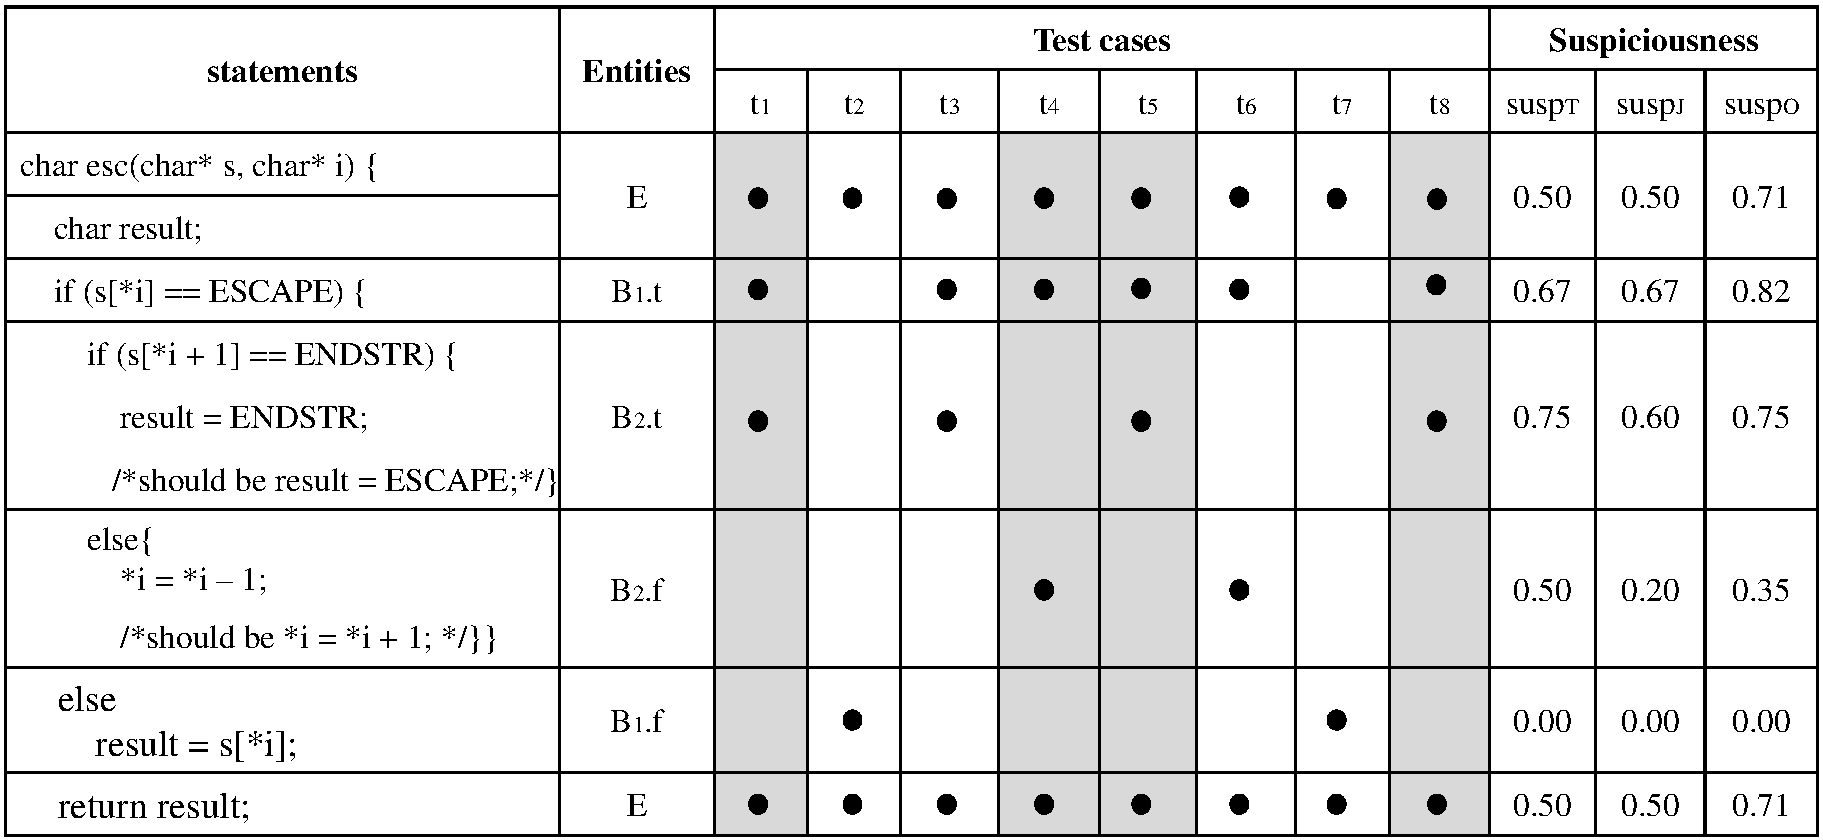
\includegraphics[width=0.95\linewidth]{spectra.pdf}
      \caption{示例程序的分支覆盖特征谱}
      \label{fig:spectra}
\end{figure}

图~\ref{fig:spectra}是示例程序的分支覆盖特征谱,示例代码来自于西门子标准集
\footnote{http://sir.unl.edu/portal/index.php}。图~\ref{fig:spectra}中的示例代码共有2个嵌套的分支结
构,分别是$B_1$和$B_2$。对于每个分支结构,我们用分别用$t$和$f$来示意其两个分支,如$B_1.t$表示第一个
分支结构的真分支。根据分支情况将示例代码分为五个部分,可表示为$P = \{E, B_1.t, B_1.f, B_2.t,
B_2.f\}$,其中$E$表示程序的入口代码块。图~\ref{fig:spectra}中共有8个测试用例,每个测试用例的覆盖信息
表示为一列,黑色圆圈表示该测试用例覆盖了所对应的程序元素。灰色阴影的测试用例表示该用例的执行结果为失
效;反之则为成功用例。右边三列表示用三种经典的可疑度计算公式计算出的可疑度,分别是
Tarantula~\cite{jones2005empirical}、Jaccard~\cite{abreu2007accuracy}和
Ochiai~\cite{abreu2007accuracy}。

以图~\ref{fig:spectra}中的示例代码为例,该代码片段中存在两个缺陷$d_1$和$d_2$,分别在分支结构$B_2$的
真假分支$B_2.t$和$B_2.f$上。失效用例集为$T_f=\{t_1, t_4, t_5, t_8\}$,其中测试用例$t_1, t_5, t_8$覆
盖$d_1$,用例$t_4$覆盖$d_2$。由图~\ref{fig:spectra}可以看出,由于示例代码存在两个缺陷,导致对于每个
缺陷,都存在不覆盖该缺陷的失效用例。例如对于缺陷$d_2$,虽然被失效用例$t_4$覆盖,但是由于缺陷$d_1$的
存在,导致大多数失效用例都不需要覆盖缺陷$d_2$,因此按可疑度比实际偏低。图~\ref{fig:spectra}中的三个
可疑度计算结果可以看到,分支$B_2.f$的可疑度远远比$B_2.t$低,甚至比$E$的可疑度更低。值得注意的是,由
于分支$B_1.t$存在于两个缺陷的共同路径上,因此其被所有的失效用例覆盖,导致其可疑度比实际偏高。

为了说明缺陷个数和基于覆盖分析的可疑度计算之间的关系,本文用$\alpha$表示其被失效用例覆盖的次数占失效
用例总数的比例。当程序中只存在一个缺陷$d$时,所有失效用例均覆盖该缺陷,因此不存在未覆盖该缺陷却导致
测试用例失效的情况,$\alpha=1$永远成立;而当程序中存在不止一个缺陷时,导致测试用例失效的缺陷可能不止
一个,覆盖其中一个或多个缺陷的测试用例都有可能会触发缺陷,导致软件行为失效,因此可能存在失效用例只覆
盖其中部分缺陷,此时$\alpha<=1$;随着具有破坏程序行为能力的缺陷个数越来越多,每个缺陷所触发的失效用
例占失效用例总数比例越来越小,此时$\alpha$也随之变小。

以Tarantula\cite{jones2005empirical}为例,使用$\alpha$可将公式~\eqref{eq:tar}表示为:
\begin{eqnarray}
 susp_T = \frac{1}{1+\frac{|T_p|}{\alpha}}, \label{eq:t}
\end{eqnarray}
其中$|T_p|$表示成功用例的个数。从公式~\eqref{eq:t}中可以看出,随着软件中包含的缺陷越来越多,由于每个缺
陷所导致的失效用例占总失效用例的比例下降,导致包含缺陷的程序元素所对应的$\alpha$变小,因此缺陷的可疑
度$susp_T$降低,从而影响了缺陷定位的准确度和效率。

\subsection{多缺陷定位相关工作}
在早期研究中,有研究者提出``One-bug-at-a-time''~\cite{klahr1988cognitive},将多缺陷程序视为单缺陷程
序进行定位,在修复缺陷后若还存在失效用例,则继续缺陷定位并修复。这种方法由于忽略了缺陷之间的相互影
响,导致定位缺陷的准确率较低,且由于需要重复执行测试用例集,因此效率较低。

一种理想的解决方式是将由不同缺陷导致的失效用例划分成为不同的失效用例集,对其中每个失效用例集可视为当
前程序只存在一个可触发程序失效的缺陷,其余缺陷均不能引起程序行为失效。在这种情况下,所有失效用例均覆
盖包含缺陷的代码,此时缺陷代码的$a_{01}=0$,因此$\alpha$取得最大值。根据公式~\eqref{eq:t}可知,当
$\alpha$取最大值时,缺陷代码的可疑度最高。这种方法的优点在于每个失效用例集均来自于同一缺陷,因此测试用例的直观性比较强,使用单缺陷定位方法能够快速定位到缺陷。

为了达到这个效果,部分学者使用聚类分析将失效用例进行聚类~\cite{jones2007debugging,
zheng2006statistical},对每类失效用例采用单缺陷的方法进行处理。基于聚类分析的方法,其核心思想是由相
同缺陷引起的失效用例其程序行为相似,具有相似的覆盖信息。这种方法虽然在一定程度上提高了多缺陷的定位准
确率,但是依赖聚类分析的准确性,很难完全避免多缺陷之间的相互影响。

文万志等人~\cite{conslice2013}提出使用条件切片进行多缺陷定位,该方法根据输入条件的不同计算出不同的条
件切片,将失效用例进行划分,每类失效用例被视为由同一缺陷引发,最后通过基于覆盖分析的缺陷定位技术计算
可疑度。该方法与基于聚类分析的方法类似,其最终目的是将多缺陷程序当做单缺陷程序处理,在依赖划分准确性
的同时忽略了缺陷之间的相互影响;与之不同的是,本文方法不需要对失效用例进行划分,且不需要进行条件切
片。

基于失效用例划分的多缺陷定位方法~\cite{zheng2006statistical, jones2007debugging, conslice2013}虽然在
一定程度上提高了多缺陷定位的效率,但其准确度依赖于失效用例划分的质量。不准确的划分使得同一失效用例集
中包含来自多个缺陷的失效用例,因此容易导致混入由其它缺陷导致的失效用例,从而引入噪音;除此以外,由于
划分导致每个失效用例集的规模变小,因此可能引起缺陷定位的不准确性。

何加浪等人~\cite{neural2013}提出使用神经网络定位多缺陷,该方法通过学习输入和缺陷之间的关系,计算代码
的各个位置与每个缺陷之间的相关性来定位缺陷。该方法利用神经网络的泛化能力学习代码和缺陷的相关性,需要
提前假定程序中的缺陷个数。而在实际应用中,软件维护人员很难提前知道潜在的缺陷个数。与之不同的是,本文
方法对缺陷个数不敏感,无需假定程序中存在的缺陷个数,且计算复杂度较低,更适用于大规模软件系统。

与本文方法相近的方法是最近邻法~\cite{renieres2003fault},该方法通过对每个失效用例找出与其最相似的成
功用例,并计算两者之间的不同来推测用例失效的原因。与之不同的是,本文受数据挖掘领域的特征选择所启发,
借鉴相关统计量的概念,将缺陷代码视为对测试用例执行结果影响较大的分支覆盖特征,提出了缺陷相关统计量,使被执行
后越容易导致用例失效的代码可疑度越高。

\section{基于特征选择的缺陷定位算法}
本章在基于覆盖分析的缺陷定位技术的基础引入了相关统计量的概念,从数据挖掘的角度计算代码对程序执行结
果的重要性,通过为每个测试用例寻找距离最近的测试用例,在很大程度上避免了多缺陷相互之间的影响,提升了
缺陷定位的效率和准确率。

\subsection{基于覆盖分析的缺陷定位}
\begin{figure}[htp]
      \centering
      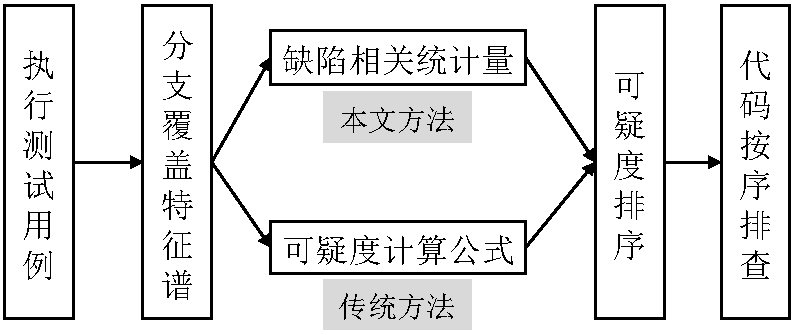
\includegraphics[width=0.6\linewidth]{fault_flow.pdf}
      \caption{覆盖分析法的基本流程}
      \label{fig:fault_flow}
\end{figure}

如图~\ref{fig:fault_flow}所示,基于覆盖分析的缺陷定位技术(以分支覆盖特征为例)主要包括以下三步:

(1)运行测试用例,收集运行过程中的分支覆盖信息,得到分支覆盖特征谱;

(2)按照特定的可疑度计算公式为每个分支计算可疑度;

(3)按照可疑度由高至低对相关进行排查。 

\begin{Definition}
      程序。程序$P$由代码表示,记作$P=\{e_1, e_2, e_3, ..., e_n\}$,其中$e$表示特定的
      程序元素。
\end{Definition}

为了收集测试用例执行的覆盖信息,首先将程序表示为由程序元素组成的序列。常用的程序元素有语句、分支、谓
词、定义对等。根据元素的粒度不同,可以将程序元素分为语句和基本块两类,前者将程序的所有语句表示成一个
序列,记录每条语句的覆盖信息;后者将程序表示为基本块序列,每个基本块由部分程序语句组成(如分支等)。
程序元素可以是基于控制流的程序语句组合(如语句、分支等),也可以是通过数据流分析提取的变量的定义-使
用对,通过关注在成功和失效用例中变量的使用情况来定位缺陷,还可以是其它与程序行为相关的关键代码,如谓
词等。程序元素的多样性使得基于覆盖分析的缺陷定位技术更加灵活和高效。

\begin{Definition}
      软件缺陷。软件缺陷是程序中存在的对程序行为具有破坏能力的错误或功能缺陷,记作$d$。
\end{Definition}

\begin{Definition}
      成功用例。执行测试用例,当且仅当程序$P$的输出与预期输出一致时,称该测试用例为成功用例,成功用
      例集记作$T_t$。
\end{Definition}

\begin{Definition}
      失效用例。执行测试用例,当程序$P$的输出与预期输出不一致时,称该测试用例为失效用例,失效用例集
      记作$T_f$。
\end{Definition}

软件缺陷是导致程序行为与预期不同的主要原因,纠错性软件维护通过查找和修复软件缺陷,提高软件系统的可靠
性。根据测试用例执行的结果是否与预期一致,可以将测试用例集划分为成功用例和失效用例两类。成功执行的测
试用例可能未覆盖软件缺陷,也可能覆盖但并未出发软件缺陷;相反,失效执行的测试用例覆盖并触发至少一个软
件缺陷,导致程序的正常行为被破坏,与预期不一致。

\begin{Definition}
      程序谱。给定程序$P$,程序谱用来表示测试用例集在程序$P$上的执行覆盖信息,记作二维矩阵
      $S_{m\times n}$,其中$m$表示测试用例集的规模,$n$为程序中所含程序元素的个数。矩阵元素$S_{ij}$
      为
      \begin{eqnarray}
         S_{ij} = \begin{cases} 1, & \mbox{第}i\mbox{个测试用例覆盖了第}j\mbox{个程序元素} \\ 
  0, & \text{ 其它 }  
  \end{cases}   , 1 \leqslant i \geqslant  m, 1 \leqslant j \geqslant n
      \end{eqnarray}
\end{Definition}

在确定程序元素后,通过插桩技术记录测试用例执行过程中是否覆盖特定的程序元素,并将结果记录在程序谱
中。需要注意的是,程序谱只记录程序元素的是否被测试用例覆盖,并不记录测试用例执行的顺序,因此程序谱通
常是二维0-1矩阵,其所占内存与测试用例集的规模和程序规模有关,通常在可接受范围内。

基于覆盖分析的缺陷定位方法,除部分结合切片技术的方法~\cite{conslice2013,wen2013}外,其大致流程通常不
变,通过改变可疑度计算公式来提高方法的准确率和效率。缺陷定位的目的是查找引起程序行为失效的程序代码。
不考虑外部因素,失效用例的执行路径至少覆盖一个软件缺陷,且不覆盖软件缺陷的测试用例一定是成功用例。因
此,是否覆盖缺陷代码与测试用例否失效之间存在一定的相关性。本文假设是否覆盖缺陷代码是判断程序行为是否
失效的重要因素,借鉴特征选择中的相关统计量概念计算代码对程序行为结果的重要性,从而定位软件缺陷。如图
~\ref{fig:fault_flow}所示,在基于覆盖分析的缺陷定位基础上,受特征选择启发,引入了相关统计量的概念,
并提出了缺陷相关统计量来计算代码的可疑度,提高了定位缺陷的额准确率和效率。

\subsection{Relief特征选择模型}

现实问题中往往存在大量的特征,然而不是所有特征都与任务目标有关。根据与任务目标的相关性,可以将特征分
为无关特征和相关特征两类。与任务目标毫无关联的特征一般被称为``无关特征'',大量的无关特征可能会导致特
征的维度过高,造成``维度灾难'',同时可能导致训练难度的提高。因此,去掉无关特征可以在降低数据维度的同
时降低训练难度,对模型训练是有益的。另一类与任务目标有关的特征通常被称为``有关特征'',然而有关特征之
间并一定是相互独立的,可能存在部分特征可以通过其它特征计算得到,这类特征通常记作``冗余特征''。虽然冗
余特征可以通过其它特征获得,但并不代表冗余特征一定是无益的。部分冗余特征通过对其它特征的整合,使得其
本身更接近学习任务,因此可以降低学习的难度。因此,冗余特征不一定要全部移除,根据特征与学习目标的关
系,可将冗余特征分为``有益特征''和``无益特征''。特征选择的目的就是去除特征集合中的与学习任务不相干的
``无关特征'',以及虽然与学习任务相关,但可以由其它特征计算而来且对学习任务没有益处的``冗余特征''。

Relief特征选择模型由Kira~\cite{kira1992feature}等人提出,最早用来针对二分类问题在数据预处理阶段进行
特征选择,从而降低数据维度。Relief特征选择模型的核心思想是通过估算特征对相似样本的区分能力来判断特征
是否对二分类学习任务有益。样本的相似性通过样本之间的距离来衡量,给定距离公式,距离越小的样本,相
似性越大。特征对相似样本的区分能力体现在,对任意一个样本以及与其最相似的同类样本和异类样本,若在某个
特征上,样本总是倾向于与同类样本的距离近,而与异类样本的距离远,则认为该特征上对相似样本具有区分能
力。

为了衡量特征对相似样本的区分能力,Kira~\cite{kira1992feature}等人引入了相关统计量的概念,计算每个特
征与二分类类别之间的相关性,并将其作为特征的权重,提出了一种基于特征权重的算法,通过移除权重低于特定
阈值的特征来进行特征选择。具体来说,给定样本集$\mathcal D=\{(x_1,y_1),(x_2,y_2),...,(x_n,y_n)\}$,和
原始特征集$\mathcal F=\{f_1,f_2,...,f_q\}$,其中$q$为原始特征的个数,
$x_i=\{x_{i1},x_{i2},...,x_{iq}\}$,。从训练样本集$\mathcal D$中随机抽取一个样本$(x_i,y_i)$,Relief
特征选择模型分别为样本$(x_i,y_i)$寻找一个同类样本$(x_{i,nh},y_i)$(记作$near-hit_i$)和一个异类样本
$(x_{i,nm},-y_i)$(记作$near-miss_i$),然后分别计算$x_i$与$x_{i,nh}$和$x_i$与$x_{i,nm}$在第$j$个特
征上的距离之差:
\begin{equation}
       \delta^j_i = -\text{diff}(x_i^j, x_{i,nh}^j)^2 + \text{diff}(x_i^j,x_{i,nm}^j)^2, \label{eq:delta}
\end{equation}
当特征$f_j$为离散型时:
\begin{equation}\label{eq:lisan}
       \text{diff}(x^j_a,x^j_b) = \begin{cases} 0, & \textit{if}~x^j_a=x^j_b \\ 
  1, & \text{ otherwise, }  
  \end{cases} 
\end{equation}
当特征$f_j$为连续型时:
\begin{equation}
       \text{diff}(x^j_a,x^j_b) = |(x^j_a-x^j_b)|.
\end{equation}
重复上述过程,从样本集中随机抽取样本$M$次,得到关于特征$f_j$的相关统计量:
\begin{equation}
       \delta^j = \frac{1}{M}\sum_{i=1}^M{-\text{diff}(x_i^j, x_{i,nh}^j)^2 + \text{diff}(x_i^j,x_{i,nm}^j)^2}. \label{eq:Delta}
\end{equation}

从公式~\eqref{eq:delta}中可以看出,在第$j$个特征上,当$x_i$与其最近同类$x_{i,nh}$距离小,与其最近异
类$x_{i,nm}$距离大时,说明此时该特征对区分不同类别的样本是有益的,因此增加特征$f_j$的权重
$\delta^j_i$;反之,若$x_i$与其最近同类$x_{i,nh}$距离大,而与其最近异类$x_{i,nm}$距离小时,说明此时
该特征对区分不同类别的样本是无益的,此时减小特征$f_j$的权重$\delta^j_i$。Relef特征选择算法为每个测试
用例寻找距离最近的同类和异类样本,距离同类越近、距离异类越远的特征被认为越能够区分不同类别的样本。

\subsection{缺陷相关统计量}
\subsubsection{基于Relief算法的缺陷定位}
借鉴特征选择中的相关统计量概念,是否覆盖缺陷代码可以被认为是对相似测试用例的执行
结果有区分能力的重要因素。缺陷定位的目的是查找能够引起程序行为失效的程序代码,因
此对缺陷代码的执行与程序行为失效之间必然存在某种关联性。不考虑外部因素,失效用例
的执行路径中应该覆盖一个或多个软件缺陷,而不覆盖任何缺陷代码的测试用例理论上一定
是成功用例。因此,是否覆盖缺陷代码与测试用例执行是否失效之间存在一定的相关性。本
文假设可以通过测试用例的执行路径来预测测试用例是否失效,因此,将测试用例在执行过
程中对代码的覆盖信息作为输入数据,测试用例的执行结果作为二分类标签,可以构建一个
二分类模型。可以通过估算覆盖特征对相似测试用例是否失效的区分能力,来选择重要的覆
盖特征,从而定位软件缺陷。需要注意的是,本章接下来以分支覆盖特征为例,但实际上本
章提出的缺陷相关统计量可用于其它程序谱,如语句、谓词、定义对等。

给定程序$P$和测试用例集$\mathcal T$,将该测试用例集作为样本数据集$\mathcal D$,
则测试用例集中的一个测试用例$T_i$可视为一个样本$\mathcal D_i=(x_i,y_i)$,其中
$x_i$表示测试用例$T_i$对代码的分支覆盖特征,用
$x_i=\{x_i^1,x_i^2,x_i^3,...,x_i^n\}$来表示,其中$n$为程序中所含分支覆盖特征的个
数,即原始特征的个数。$x_i^j$为:
\begin{equation}\label{eq:cov}
      x_i^j = 
       \begin{cases}
             1, & \mbox{测试用例}T_i\mbox{覆盖第}j\mbox{个程序元素}\\ 
  0, & \mbox{测试用例}T_i\mbox{未覆盖第}j\mbox{个程序元素},  
       \end{cases}
\end{equation}
也是样本的原始特征;$y_i$表示测试用例$T_i$的执行结果(成功或失效),也是样本的标签$y_i$:
\begin{equation}
      y_i = 
       \begin{cases}
             1, & T_i\mbox{是成功用例}\\ 
  -1, & T_i\mbox{是失效用例}.  
       \end{cases}
\end{equation}

\subsubsection{存在的问题}

结合基于覆盖分析的缺陷定位技术,本文认为缺陷代码的覆盖信息与测试用例执行的结果应该有以下相关性:
\begin{itemize}
      \item 失效用例的执行路径覆盖至少一个缺陷;
      \item 不覆盖缺陷代码的测试用例一定是成功用例;
      \item 被失效用例覆盖越多、成功用例覆盖越少的代码越有可能是缺陷代码。
\end{itemize}

本章在基于覆盖分析的缺陷定位基础上,受特征选择启发,引入了相关统计量的概念来定位缺陷。相关统计量最早
被用来做二分类之前的特征选择,其主要思路是将对相似样本有区分能力的特征作为重要的特征。当使用相关统计
量来进行缺陷定位时,根据公式~\eqref{eq:Delta},特征$f_j$的相关统计量$\delta^j$较高的可能存在以下四种原
因:当$x_i^j=0$时,$y_i=1$总是成立;当$x_i^j=0$时,$y_i=-1$总是成立;当$x_i^j=1$时,$y_i=1$总是成
立;当$x_i^j=1$时,$y_i=-1$总是成立。换言之,相关统计量所代表的含义仅仅是特征与分类结果的相关性,而
与测试用例执行结果相关的代码并不一定包含缺陷代码,直接使用特征选择的概念来计算相关统计量,容易导致以
下代码的相关统计量偏高:

a. 当测试用例的执行路径未覆盖某个分支时,测试用例总是成功执行;

b. 当测试用例的执行路径未覆盖某个分支时,测试用例总是失效执行;

c. 当测试用例的执行路径覆盖某个分支时,测试用例总是成功执行;

d. 当测试用例的执行路径覆盖某个分支时,测试用例总是失效执行。

根据公式~\ref{eq:Delta},上述四种可能中的代码对测试用例执行结果的区分能力较强,因此相关统计量较高。
然而,这与定位缺陷代码的目的并不完全一致。虽然覆盖缺陷代码与测试用例执行结果是否失效存在一定的关联
性,但是相关统计量高的代码未必可疑度高,因为对测试用例的执行结果有较强区分能力的代码包括但并不完全等
价于覆盖后容易导致测试用例失效执行的代码。具体来说,根据缺陷分支覆盖特征与测试用例执行结果的相关性,
在上面的四种相关统计量较高的可能情况中,只有a和d两种情况暗示着该分支有较大可能是缺陷相关分支,而b和c
两种情况则完全相反,暗示着该分支很有可能是缺陷无关分支。

\subsubsection{缺陷相关统计量}

Relief算法中的相关统计量只用来衡量特征与二分类结果的相关性,而并未给出特征是如何
影响分类结果的。为了研究相关统计量与代码可疑度之间的关系,本文提出缺陷相关统计量
的概念来度量代码与缺陷的相关性,并以此作为代码的可疑度。首先,由于测试用例的执行
路径只有``覆盖''和``不覆盖''某个程序元素两种可能,因此分支覆盖特征是离散型0-1变
量,我们将公式~\eqref{eq:lisan}代入公式~\eqref{eq:delta}可得相关统计量为:
\begin{equation}
       \delta^j_i = -\llbracket x_i^j \neq x_{i,nh}^j \rrbracket + \llbracket x_i^j \neq x_{i,nm}^j \rrbracket, \label{eq:delta2}
\end{equation}
从公式~\eqref{eq:delta2}中可以看出,给定分支$f_j$,随机抽取一个测试用例$x_i$并寻找距离该用例最近的一个
同类用例$x_{i,nh}$(near-hit)和一个异类用例$x_{i,nm}$(near-miss)。只要在分支$f_j$上$x_{i,nh}$与
$x_i$的覆盖情况相同,而$x_{i,nm}$与$x_i$的覆盖情况不相同,则有$\llbracket x_i^j \neq x_{i,nh}^j
\rrbracket=0$,$\llbracket x_i^j \neq x_{i,nm}^j \rrbracket=1$,此时$\delta_i^j=1$,增加分支$f_j$的
相关统计量$\delta^j$。

考虑一种情况,当随机抽取的测试用例$x_i$是失效用例($y_i=-1$)时,若此时$x_i^j=x_{i,nh}^j=0$,且有
$x_{i,nm}=1$,则按照公式~\eqref{eq:delta2}可得,此时$\delta_i^j=1$,应该增加相关统计量$\delta^j$。然
而,在这种情况下,失效用例$x_i$和$x_{i,nh}$均未覆盖第$j$个代码块,反而成功用例$x_{i,nm}$覆盖了第$j$
个代码块。根据代码被失效执行越多、成功执行越少则可疑度越高的原理,此时减少覆盖分支$f_j$的可疑度。

由此可以看出,Relief算法中相关统计量的更新只与样本和最近同类、异类样本的距离有关,而缺陷定位中覆盖特
征的可疑度的更新还需要考虑随机抽取的测试用例$x_i$的类别$y_i$(成功或失效)以及其是否覆盖分支$f_j$。本文与传统的覆盖分析法基于类似的思想,即被失效用例覆盖越多、成功用例覆盖越少的代码可疑度越
高。因此,根据随机抽取测试用例的类别和对分支$f_j$的覆盖情况不同,可分为以下四种情况:

(1)当随机抽取的测试用例为失效用例且未覆盖分支$f_j$时,若此时$\delta_i^j$较大,则说明分支
      $f_j$同样未被相似的失效用例所覆盖,而是被相似的成功用例所覆盖,此时应该减小分支$f_j$的可疑度;

(2)当随机抽取的测试用例为失效用例且覆盖了分支$f_j$时,若此时$\delta_i^j$较大,则说明分支$f_j$同样被相似的失效用例所覆盖,且未被相似的成功用例所覆盖,此时应该增加分支$f_j$的可疑度;

(3)当随机抽取的测试用例为成功用例且未覆盖分支$f_j$时,若$\delta_i^j$较大,则说明此时分支$f_j$未被相似的成功用例所覆盖,而是被相似的失效用例所覆盖,因此应该增加分支$f_j$的可疑度;

(4)当随机抽取的测试用例为成功用例且覆盖了分支$f_j$时,若$\delta_i^j$较大,则说明此时分支$f_j$同样被相似的成功用例所覆盖,且未被相似的失效用例所覆盖,因此应该减小分支$f_j$的可疑度。

表~\ref{tbl:list}中总结了在不同的情况下,相关统计量与可疑度的关系:
\begin{center}
\zihaowu
\tablecaption{相关统计量与可疑度的关系}\label{tbl:list}
\begin{tabular}{lll}
\toprule
测试用例 & 是否覆盖分支$f_j$ & 相关统计量$\delta^j$与可疑度$\epsilon^j$的关系\\ \midrule
\multirow{2}{*}{失效用例} & 未覆盖 & $\epsilon^j$随着$\delta^j$的增加而减小\\
& 覆盖 & $\epsilon^j$随着$\delta^j$的增加而增加\\ \midrule
\multirow{2}{*}{成功用例} & 未覆盖 & $\epsilon^j$随着$\delta^j$的增加而增加\\
& 覆盖 & $\epsilon^j$随着$\delta^j$的增加而减小\\ 
\bottomrule
\end{tabular}
\end{center}

表~\ref{tbl:list}中的$\epsilon^j$表示分支$f_j$的可疑度。可以看出,随机抽取测试用
例后,对每个分支的可疑度的更新与该测试用例是否成功执行以及是否覆盖该分支有关。根
据表~\ref{tbl:list},本文提出了缺陷相关统计量$\epsilon$来估算可疑度。给定分支
$f_j$,随机抽取测试用例$(x_i,y_i)$后,关于分支$f_j$在测试用例$(x_i,y_i)$上缺陷相
关统计量为:
\begin{equation}
       \epsilon_i^j = -y_ix_i^j(-\llbracket x_i^j \neq x_{i,nh}^j \rrbracket + \llbracket x_i^j \neq x_{i,nm}^j \rrbracket). \label{eq:epsilon}
\end{equation}

最后通过从样本集$\mathcal D$中随机抽取样本M次并重复上述计算过程,可得到关于分支
$f_j$的缺陷相关统计量:
\begin{equation}
       \epsilon^j = \frac{1}{M}\sum_{i=1}^M{ -y_ix_i^j(-\llbracket x_i^j \neq x_{i,nh}^j \rrbracket + \llbracket x_i^j \neq x_{i,nm}^j \rrbracket)}. \label{eq:epsilon2}
\end{equation}

需要注意的是,在随机抽取一个测试用例$(x_i,y_i)$后,按照算法~\ref{alg:relief}的第
8行,需要在成功用例集$\mathcal D^+$和失效用例集$\mathcal D^-$中分别寻找一个举例
该测试用例最近的用例。根据公式~\eqref{eq:cov},测试用例的特征$x_i^j$可作为布尔值,
因此本文使用曼哈顿距离来计算测试用例$x_a$和$x_b$之间的距离:
\begin{equation}
      \text{distance}(x_a,x_b) = \sum_{i=1}^n{|x_a^i-x_b^i|}
\end{equation}

算法~\ref{alg:relief}为本文提出的缺陷相关统计量的算法,基于Relef特征选择的思想,为每个测试用例寻找距
离最近的同类和异类样本,距离同类越近、距离异类越远的特征被认为越能够区分不同类别的样本。从算法
~\ref{alg:relief}中可以看出计算缺陷相关统计量所需的运行时间与原始特征集的规模$|\mathcal F|$和样本的
随机抽样次数$M$线性相关,因此该算法的效率较高。

\begin{algorithm}[H]
\caption{缺陷相关统计量算法}\label{alg:relief}
\KwIn{样本数据集$\mathcal D$,覆盖特征集合$\mathcal F$,缺陷相关统计量阈值$\Gamma$,采样次数$M$;}\\
\KwOut{缺陷相关统计量向量$\delta$;} \\
初始化每个覆盖特征的缺陷相关统计量$\bm \delta^j \leftarrow \bm 0$;\\ 
根据样本标签将样本数据集$\mathcal D$划分为正类$\mathcal D^+$和负类$\mathcal D^-$;\\
\For {$i=1$ to $|M|$} {
     从样本数据集$\mathcal D$中随机抽取一个样本$(x_i,y_i)$;\\
     从子数据集$\mathcal D^+$和$\mathcal D^-$中分别寻找距离$x_i$最近的两个样本,其中与$(x_i,y_i)$同类的样本为$(x_{i,nh},y_i)$,与$(x_i,y_i)$异类的样本为$(x_{i,nm},y_i)$;\\
     \For {$j=1$ to $|\mathcal F|$} {根据当前样本$(x_i,y_i)$计算在覆盖特征$f_j$的缺陷相关统计量
            $\delta^j_i$(公式~\eqref{eq:epsilon});\\
            更新覆盖特征$f_j$的缺陷相关统计量$\delta^j \leftarrow \delta^j + \delta^j_i$;\\
     }
}
\For{$j=1$ to $|\mathcal F|$} {
      计算覆盖特征的平均缺陷相关统计量$\delta^j \leftarrow \frac{\delta^j}{M}$;\\
}
\textbf{return} 缺陷相关统计量向量$\delta$。\\
\end{algorithm}

\subsection{代码排查}\label{code_search}
如图~\ref{fig:fault_flow}所示,在获得测试用例集$\mathcal T$对程序$P$执行过程中的
分支覆盖信息后,本文将以测试用例作为样本数据,提出了缺陷相关统计量,利用算法
~\ref{alg:relief}估算分支特征的可疑度(算法~\ref{alg:relief}中的第10行改为缺陷相
关统计量公式~\eqref{eq:epsilon}),最后按照可疑度由高至低按需排查相关代码。

给定程序$P$,在执行测试用例集后,收集分支覆盖信息得到如图~\ref{fig:spectra}所示的分支覆盖特征谱,利用
Relief算法~\ref{alg:relief}计算分支特征的相关统计量,并提出缺陷相关统计量的计算方式(公式
~\eqref{eq:epsilon2})来代替原有的相关统计量,并将所有分支特征按照缺陷相关统计量由高至低排序,得到分支
覆盖特征序列$\mathcal B=\{B_1,B_2,B_3,...,B_n\}$,最后按照可疑度由高至低进行排查。

算法~\ref{alg:search}为根据分支覆盖特征的可疑度排查代码的算法。以图~\ref{fig:spectra}中的分支$B_2.f$
为例,由于$B_2.f$为分支结构$B_2$的一个分支,因此首先排查其所在分支结构$B_2$的判定语句,即第4行语句;
由于不存在与该判定语句在同一个基本块且可以影响到判定结果的语句,因此直接检查分支$B_2.f$中的可执行语
句(*i=*i-1)。

\begin{algorithm}[H]
\caption{代码排查算法}\label{alg:search}
\KwIn{程序$P$,分支覆盖特征序列$\mathcal B$;}\\
\For {$i=1$ to $|B|$} {
      //对分支覆盖特征$B_i$进行排查 \\
      \If{$B_i$是分支结构的一个分支}{
            排查$B_i$所在分支结构的判定语句$S_j$;\\
            排查与判定语句$S_j$在一个基本代码块内,且可能影响到其判定结果的语句;\\
            排查在$B_i$内且控制依赖于分支$B_i$的语句;\\
      }
      \Else{
            排查与$B_i$同在一个函数的所有必须被执行的可执行语句,包括部分分支结构的判定语句;\\
      }
}
\end{algorithm}

\section{实验设计}
本节评估了基于相关统计量的缺陷定位技术和其它主流的基于覆盖分析的缺陷定位方法的有效性,设计了两组实
验,分别针对单缺陷程序和多缺陷程序进行错误定位,在开源数据集上通过对比实验验证了本文方法的有效性。

\subsection{实验对象}\label{subjects1}

为了评估缺陷定位方法的有效性,选取了来自开源软件仓库~\footnote{http://sir.unl.edu/portal/index.php}
(Software Infrastructure Repository,以下简称SIR)的Siemens程序集和flex程序作为实验对象。表
~\ref{tbl:subjects1}中列出了本次实验中实验对象的相关统计数据。


\begin{center}
\zihaowu
\tablecaption{实验对象}\label{tbl:subjects1}
\begin{tabular}{ccccc}
\toprule
实验程序 & 代码行数 & 缺陷版本数量 & 测试用例数量\\ \midrule
print\_tokens & 563 & 3 &4130\\ 
print\_tokens2 & 508 & 8 & 4115\\ 
replace & 563 & 28 & 5542\\ 
schedule & 410 & 6 & 2650\\ 
schedule2 & 307 & 4 & 2710\\ 
tot\_info & 406 & 20 & 1052\\ 
tcas & 173 & 39 & 1608\\ 
flex & 12\textasciitilde14k & 51 & 567\\ \bottomrule
\end{tabular}
\end{center}

其中,Siemens程序集经常作为基准程序集用来评估缺陷定位方法的有效性~\cite{guanlian2013,con-prob2018},
包括7个C语言程序,其中print\_tokens和print\_tokens2为词法分析器,replace为一个模式替换程序,schedule
和schedule2为两个优先级调度程序,tot\_info可用来进行信息度量,tcas为ADL解释器。除程序源代码外,SIR提
供了植入缺陷的程序版本以及测试用例集。除了Siemens程序集外,使用flex词法分析器来评估方法的有效性。由
于flex是Unix系统中真实使用的程序,因此除了植入的缺陷外,其中还包含部分真实存在的软件缺陷。从表
~\ref{tbl:subjects1}中可以看出,Siemens程序集中的代码行数在170\textasciitilde565之间,属于小规模程
序,而flex的代码行数在12\textasciitilde14k之间,属于大规模程序。

需要注意的是,表~\ref{tbl:subjects1}中所列的缺陷版本数量为经过筛选后的缺陷版本。跟传统的基于覆盖分析
的缺陷定位研究相似,本文在选择缺陷程序版本的时候,进行以下筛选:(1)排除了无法被现有测试用例集所触
发的缺陷版本,即在现有测试用例在执行该缺陷版本时均为成功用例,无法根据测试用例的执行结果判断此时是否
存在缺陷;(2)排除了由代码缺失引起的缺陷,因为基于覆盖分析的缺陷定位研究通常根据代码的覆盖信息与测
试用例的执行估算代码的可疑度,而缺失的代码既不会有覆盖信息,也不存在相应的可疑度,因此在评估方法有效
性时存在问题;(3)排除了有可能引起程序运行时出现异常(segment fault),导致程序运行突然中止的缺陷,
由于基于覆盖分析的缺陷定位技术依赖于测试用例集在整个程序执行过程中对代码的覆盖信息,而可能出现异常中
止的程序导致部分测试用例的覆盖信息不完全,在计算可疑度的时候与其它测试用例不一,因故在实验中将这部分
缺陷排除。最后在实验中一共使用了108个缺陷,并在实验中通过控制一个程序中所注入缺陷的个数来分别构造单
缺陷和多缺陷的程序。

\subsection{评估方法}
本章在ubuntu14.10系统下进行实验,使用的gcc编译器版本为4.4.1。在执行测试用例之前,使用开源语法分析工
具antlr(版本为3.5.1)在程序的入口和各个分支处进行插桩。然后,通过脚本执行SIR提供的测试用例集,并用
antlr收集分支覆盖信息,得到分支覆盖特征谱。通过比较测试用例在程序的正确版本和缺陷版本上的执行结果是
否相同,判定测试用例为成功用例或失效用例。

缺陷定位技术的目的是帮助软件维护人员尽快找到缺陷相关代码,因此缺陷定位技术的有效性和效率通常体现在如
何通过排查尽可能少的代码,尽快定位到缺陷相关代码。基于覆盖分析的缺陷定位技术,通常根据覆盖特征谱按照
特定计算公式计算代码的可疑度,然后按照可疑度由高至低排查相关代码。因此,为了尽可能排查较少的代码,缺
陷相关代码的可疑度排名通常越高越好。

为了评估方法的有效性,本章使用定准率$\beta$和排查率$P_{search}$两个度量方式来从不同的角度对方法进行
比较。定准率表示定位到缺陷相关语句所不需要检查的代码的比例,可表示为:
\begin{equation}
       \beta = \frac{L-L_s}{L-1},\label{eq:beta}
\end{equation}
其中$L$表示程序中可执行代码的总行数,$L_s$为定位到某个缺陷所需要排查的可执行代码的总行数。从公式
~\eqref{eq:beta}中可以看出,给定程序$P$,程序中的可执行代码总数固定后,定位到缺陷所需要排查的行数越
小,定准率越高。从公式~\eqref{eq:beta}中可以看出,缺陷定位技术并不一定会提高定位缺陷的效率,当定准率
$\beta$小于一定阈值时,反而会降低定位缺陷的效率。例如,当$\beta$小于缺陷按照代码执行顺序所在的相对位
置比时,利用缺陷定位方法查找缺陷的效率比按照代码执行的顺序逐步排查更低。

代码排查率$P_{search}$表示定位到缺陷所需要排查的代码行数与可执行代码总行数的百分比,可表示为:
\begin{eqnarray}
      P_{search}=\frac{|L_s|}{L}\times100\%
\end{eqnarray}
与定准率相反,当缺陷个数固定时,代码排查率越低表示定位到缺陷所需要排查的可执行代码比例越小,因此缺陷
定位效率越高。

\subsection{对比实验}
为了评估方法的有效性设计了两组实验,分别针对单缺陷和多缺陷程序进行对比实验。由于基于相关统计量的方法
与基于覆盖分析的缺陷定位方法类似,都只需要收集测试用例对程序的覆盖信息以及执行结果,因此本章只与基于
覆盖分析的缺陷定位技术相比较。其它流行的缺陷定位技术,如基于程序切片的方法~\cite{}等,大多结合了传统
的程序动态或静态分析方法,虽然在准确度上得到了一定的提高,但也增加了缺陷定位的成本。基于覆盖分析的缺
陷定位方法,由于其计算复杂度较低,因此对于大规模软件系统有较高的适用性。

\textbf{(1)单缺陷程序对比实验}

在面向单缺陷程序的实验中,选取了5种典型的基于覆盖分析的定位方法,分别是
Tarantula~\cite{jones2005empirical}、Jaccard~\cite{abreu2007accuracy}、
Ochiai~\cite{abreu2007accuracy}以及基于最近邻的交集和并集算法~\cite{renieres2003fault}进行比较。其
中,Tarantula基于被失效用例覆盖越多、成功用例覆盖越少的测试用例越有可能是失效用例的经典假设,Jaccard
和Ochiai是两个相关系数。基于最近邻的方法与本文方法较为相近,其通过为每个失效用例寻找最相似的成功用例
来进行缺陷定位。与之不同的是,本文受Relief特征选择启发,通过选择对测试用例执行结果影较大的覆盖特征来
定位缺陷,因此本文对每个失效用例分别找出其最相似的成功和失效用例,根据它们在特征上的距离动态调整特征
的相关统计量。

\textbf{(2)多缺陷程序对比实验}

在面向多缺陷程序的实验中,选取了两种面向多缺陷程序的缺陷定位策略,分别是``One-bug-at-a-time''策略
~\cite{klahr1988cognitive}和基于聚类分析的多缺陷定位方法~\cite{jones2007debugging}。前者使用
Tarrantula、Jaccard、Ochiai三种方法计算可疑度后,每次只定位并修复一个缺陷,若修复后还存在失效用例,
则继续进行缺陷定位与修复,直至所有用例都成功执行;后者使用聚类分析将测试用例划分成不同簇,将同一簇内
的失效用例视为由同一缺陷引起的,然后当作单缺陷程序处理。基于聚类分析的方法与基于相关统计量的方法基于
相似的假设,即由同一缺陷引起的失效用例在覆盖信息上具有一定的相似性。然而,与基于聚类分析的方法不同的
是。本章方法在上述假设上添加了约束,即针对每一个失效用例,本方法认为只有距离其最近的失效用例与其为同
一缺陷导致的,在很大程度上避免了对来自不同缺陷的失效用例的误判,同时也避免了对聚类分析的准确性的依
赖。

\section{实验结果与分析}
本节从单缺陷程序和多缺陷程序两个角度对基于相关统计量的缺陷定位方法的有效性进行评估,阐述了在开源程序
Siemens程序集和Unix程序flex上进行对比实验结果,并对实验的结果进行分析。

\subsection{单缺陷程序}
单缺陷程序上的对比实验数据集总共包括来自Siemens程序集和flex词法分析器的108个缺陷程序,每个缺陷程序上
只包含一个缺陷。由于Siemens程序集和flex的软件规模不同(相差两个数量级),为了综合评估在这两种程序集
上的表现效果,使用$P_{search}$来表示已经排查的代码占可执行代码总行数的百分比,通过比较$P_{search}$小
于某个阈值时不同缺陷定位技术发现的缺陷的总数来比较这些方法的优劣,发现的缺陷越多,越说明该方法能够帮
助找到缺陷。

\begin{center}
\zihaowu
\tablecaption{单缺陷程序定位效果比较}\label{tbl:single}
\begin{tabular}{ccccccc}
\toprule
$P_{search}$(\%) & REL & TAR & JAC & OCH & UNI & INT\\ \midrule
0\textasciitilde1 & 21 & 14 & 14 & 18 & 7 & 1 \\ 
1\textasciitilde5 & 28 & 18 & 20 & 24 & 11 & 0 \\ 
5\textasciitilde10 & 18 & 19 & 20 & 18 & 6 & 5 \\ 
10\textasciitilde20 & 17 & 16 & 13 & 16 & 16 & 10 \\ 
20\textasciitilde30 & 8 & 9 & 10 & 12 & 19 & 7 \\ 
30\textasciitilde40 & 6 & 10 & 10 & 4 & 21 & 17 \\ 
40\textasciitilde50 & 2 & 4 & 5 & 5 & 15 & 24 \\ 
50\textasciitilde60 & 3 & 4 & 4 & 6 & 8 & 21 \\ 
60\textasciitilde70 & 3 & 1 & 4 & 1 & 2 & 15 \\ 
70\textasciitilde80 & 0 & 6 & 3 & 2 & 1 & 6 \\ 
80\textasciitilde90 & 2 & 3 & 2 & 0 & 2 & 1 \\ 
90\textasciitilde100 & 0 & 4 & 3 & 2 & 0 & 1 \\ 
\bottomrule
\end{tabular}
\end{center}

表~\ref{tbl:single}中统计了随着$P_{search}$的增长排查到缺陷的个数,其中缺陷定位方法从左到右依次为基
于相关统计量的方法、Tarantula、Jaccard、Ochiai、并集算法Union和交集算法Intersection。前4中方法根据可
疑度(缺陷相关统计量)的大小,由高至低排查缺陷相关代码;后面两种方法根据之前的研究~\cite{wen2013},
首先排查集合范围内的代码,然后按照失效用例的执行路径顺序排查代码。为了公平比较前4种可疑度计算方法的
有效性,本文对这4种方法均使用分支覆盖特征谱进行定位,然后按照算法\ref{alg:search}排查代码。最后,由
于缺陷定位技术只有在早期排查到缺陷相关代码时被认为时对缺陷定位有帮助,且大多数缺陷定位技术在刚开始定
位时有较密集的缺陷发现,因此在表~\ref{tbl:single}中放大了前10\%的缺陷定位效果,将其分别表示成
0\%\textasciitilde1\%、1\%\textasciitilde5\%、5\%\textasciitilde10\%三部分。

从表~\ref{tbl:single}中可以看出,两种基于最近邻的方法相比其它基于覆盖分析的方法定位缺陷的效率更低,
其中交集的表现最差。通过分析交集方法中集合中的代码,发现被所有成功用例覆盖且不被失效用例覆盖的代码很
少,且大多数情况下缺陷相关代码都不在集合内。并集方法(Union)将被失效用例覆盖且不被所有成功用例覆盖
的代码放入集合中,忽略了即使测试用例执行了缺陷代码,却有可能不触发缺陷导致失效用例的可能性,因此部分
缺陷代码被排除在集合外,同时对于集合内的代码没有进一步考虑代码的排查顺序,导致其定位效率低于其它基于
覆盖分析的缺陷定位技术。

根据表~\ref{tbl:single},基于覆盖分析的缺陷定位技术Tarantula、Jaccard和Ochiai定位的效率明显高于两种
基于集合的方法。通过对实验结果的分析,发现基于覆盖分析的缺陷定位技术在单缺陷程序中的表现较好,这是由
于当程序中只存在一个缺陷时,失效用例理论上一定覆盖缺陷代码,因此缺陷代码通常是被失效用例覆盖最多的代
码。基于覆盖分析的缺陷定位技术其核心思想是``被失效用例覆盖越多、成功用例覆盖越少的代码越有可能是缺陷
代码'',因此被失效用例覆盖最多的代码可疑度往往较高;然而同时,由于缺陷代码也可能被成功用例所覆盖,受
成功用例的约束导致在部分情况下缺陷代码的可疑度降低,从而影响定位的效率。通过固定$P_{search}$比较定位
到缺陷的个数可以发现,在缺陷定位的早期,基于相关统计量的方法定位到缺陷的数量较多。尤其是当
$P_{search}$小于\%20时,根据缺陷相关统计量可以定位到84个缺陷,说明了基于相关统计量的缺陷定位方法的有
效性。通过分析单缺陷程序,可以发现在计算缺陷代码的相关统计量时,由于所有失效用例都需要覆盖该代码,导
致公式~\eqref{eq:epsilon2}中的第一项始终为0,因此缺陷代码的相关统计量较高。

\subsection{多缺陷程序}
由于多缺陷程序中,引起测试用例失效的缺陷不止一个,缺陷代码可能不被失效用例所覆盖,因此基于覆盖分析的
方法在面对多缺陷程序时往往效率低于单缺陷程序。基于相关统计量的方法与基于覆盖分析的方法所需要的信息相
同,均只需要覆盖信息而不需要进行程序分析,因而基于相关统计量的方法可以被视为是基于覆盖分析方法的一种
特例,即不通过特定的可疑度计算公式,而是通过数据挖掘中特征选择的思想进行缺陷定位。为了让基于覆盖分析
的缺陷定位方法同样适用于多缺陷程序,有研究者提出了两种策略,分别是
``One-bug-at-a-time''~\cite{klahr1988cognitive}和基于聚类分析的并行算法~\cite{jones2007debugging,
zheng2006statistical},这两种方法的核心思想仍然是将失效用例集当作或是处理成由同一缺陷引起的失效用
例。为了评估基于相关统计量的缺陷定位方法的性能,将本文方法与上述两种基于覆盖分析的多缺陷定位方法进行
比较。同样,为了实验的公平性,所有模型均使用相同的分支覆盖特征谱。除此以外,由于Tarantula、Jaccard、
Ochiai具有相近的表现,因此在多缺陷程序的实验中选取表现略由于其它两种可疑度计算公式的Ochiai作为除本文
方法外的两个方法的可疑度计算公式。

由于Siemens程序集的规模较小且包含了植入的缺陷,因此本节使用Unix系统中的真实程序flex词法分析器作为实
验对象,通过控制flex中真实缺陷的个数,来评估缺陷定位方法在处理多缺陷程序时的有效性。本节使用
flex~1.1.1版本中的$F_HD$类型的缺陷来进行实验,在按照~\ref{subjects1}中的方法对缺陷进行筛选后,共
有6个可以被触发且没有明显相关性的缺陷,将这6个缺陷排列组合可以得到不同的缺陷版本。例如,从这些缺陷里
任意选择2个缺陷注入正确版本中,一共得到15个包含2个缺陷的程序版本。通过这种方式,得到多个缺陷版本,每
个缺陷版本中包含2\textasciitilde5个缺陷。在这些缺陷程序上进行实验,并计算平均定准率得到如表
~\ref{tbl:multi-flex}所示的结果。

\begin{center}
\zihaowu
\tablecaption{Flex多缺陷版本平均定准率$\beta$}\label{tbl:multi-flex}
\begin{tabular}{ccccccc}
\toprule
缺陷数量 & 缺陷版本数量 & REL & ONE-OCH & PAR-OCH \\ \midrule
2 & 15 & 0.87 & 0.81 & 0.82  \\ 
3 & 20 & 0.82 & 0.71 & 0.75  \\ 
4 & 15 & 0.83 & 0.64 & 0.69  \\ 
5 & 6 & 0.79 & 0.52 & 0.63  \\ 
\bottomrule
\end{tabular}
\end{center}

表~\ref{tbl:multi-flex}中的三种多缺陷定位方法从左往右依次是基于相关统计量的方法(REL)、使用Ochiai计
算可疑度的``One-bug-at-a-time''(ONE-OCH)和同样使用Ochiai的基于聚类分析的并行算法(PAR-OCH)。从表
~\ref{tbl:multi-flex}中可以看出,ONE-OCH在缺陷个数较少的时候有着与PAR-OCH相近的表现,然而随着缺陷个
数的增加,ONE-OCH的平均定准率迅速下降。当程序中存在5个缺陷时,ONE-OCH方法的平均定准率为0.52,此时缺
陷定位的效率较低,反而有可能会降低查找缺陷的速度,因此不适合使用该缺陷定位方法。PAR-OCH方法使用聚类
分析对测试用例进行聚类,其目的是当程序中存在不止一个缺陷时,可以将由不同缺陷引发的失效用例划分成不同
的簇,然后对每簇当做只存在一个缺陷进行定位。从表~\ref{tbl:multi-flex}中可以看出,该方法相比ONE-OCH方
法的平均定准率有所提高,然而当缺陷个数逐渐增加时,该方法的效率也随之迅速降低。通过分析实验数据,发现
虽然PAR-OCH方法希望将相同缺陷引起的失效用例划分为一簇,但事实上基于聚类分析的划分并不能很好地保证这
一点,尤其当缺陷个数增加时,存在很多被错误划分的失效用例,导致定位效率的下降。

\begin{figure}
\centering
\subfigure[2个缺陷]{\label{fig:temp_nuh}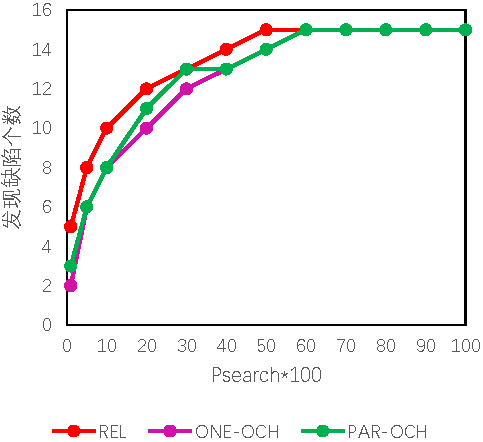
\includegraphics[width=0.49\linewidth]{fault2.pdf}}
\hfill
\subfigure[3个缺陷]{\label{fig:temp_synpuf}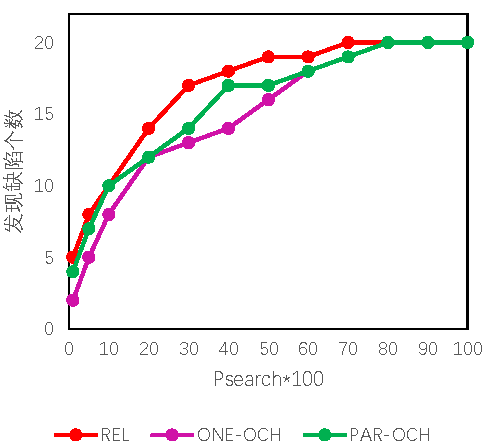
\includegraphics[width=0.49\linewidth]{fault3.pdf}}
\vskip\baselineskip
\subfigure[4个缺陷]{\label{fig:temp_nuh}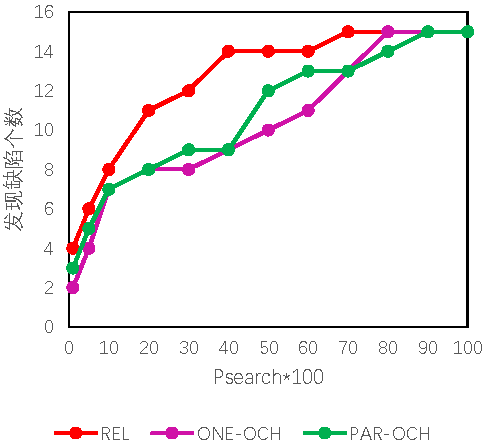
\includegraphics[width=0.49\linewidth]{fault4.pdf}}
\hfill
\subfigure[5个缺陷]{\label{fig:temp_synpuf}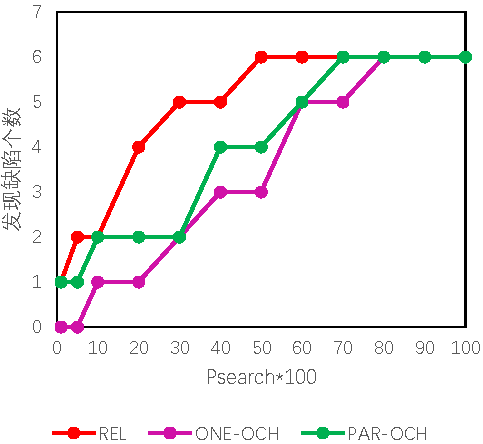
\includegraphics[width=0.49\linewidth]{fault5.pdf}}
\caption{基于覆盖分析的多缺陷定位方法的实验结果}
\label{fig:multi}
\end{figure}

图~\ref{fig:multi}更直观地表示了三种基于覆盖分析的多缺陷定位方法的效率,其中横坐标为
$P_{search}*100$,纵坐标为在一定$P_{search}$的范围内找到的缺陷的个数。可以看出,当缺陷个数较少时,三
种方法的定位效率均较高,体现在当$P_{search}$小于20\%时,三种方法可以定位到的缺陷相对密集,对缺陷定位
的帮助较大。然而,随着缺陷个数的增加,ONE-OCH定位缺陷的效率迅速降低。而当程序内缺陷个数为5时,从表
~\ref{fig:multi}中可以看出,ONE-OCH定位缺陷的个数与$P_{search}$几乎呈现线性关系,表明此时这两种方法
所推荐的代码优先级与缺陷的相关性较小,找到缺陷的个数主要依赖于代码检查量本身。

与ONE-OCH相比,PAR-OCH虽然在一定程度上提高了多缺陷定位的效率,但是通过分析实验结果发现,由于依赖聚类
分析中对测试用例划分的准确性,导致面对多缺陷程序时该方法的效果仍然不是很理想。虽然基于相关统计量的缺
陷定位方法与基于聚类分析的方法是具有相似的假设,即由相同缺陷引起的失效用例具有一定的相似性,但本文方
法在该假设上加了较强的约束,即本文认为只有距离失效用例最近的失效用例对才有很大概率由相同缺陷引起,因
此本文方法具有更高的定位准确性,同时避免了对聚类分析准确性的依赖,且不需要对缺陷的个数进行假设。

与上述两种方法相比,虽然基于相关统计量的方法定位效率同样随着缺陷个数的增加而有所降低,但由于降低的幅
度较小,因此当缺陷个数较多时,体现出了一定的优势。通过分析实验数据发现,当缺陷个数增加时,基于相关统
计量的方法只考虑与失效用例距离最近的失效用例,而两个覆盖信息极为相似的失效用例由相同缺陷引发的概率较
高,导致这两个失效用例对与它们相关的缺陷代码大多具有相同的覆盖特征,根据公式~\eqref{eq:epsilon2},此时
缺陷相关统计量较高,因此缺陷代码的优先级较高,提高了定位效率。

\subsection{适用性讨论}

\textbf{(1)覆盖特征谱}

本章以分支覆盖特征谱为例在~\ref{motivation1}对研究动机进行阐述,而实际上多缺陷定位中缺陷之间的相互影
响导致效率的降低不止是发生在分支覆盖特征谱中,在以其它覆盖特征谱(如语句、定义对等)为基础的基于覆盖
分析的多缺陷定位方法中也同样存在。同样,本章以分支覆盖特征谱为例,提出了基于相关统计量的缺陷定位方
法,但该方法也同样适用于其它覆盖特征谱。当使用其它覆盖特征谱时,仅仅改变了输入特征,仍然可以使用本文
方法进行缺陷定位。值得注意的是,当完成对覆盖特征的缺陷相关统计量的计算时,由于覆盖特征的改变,根据缺
陷相关统计量的顺序对相关代码进行排查时,将不再使用~\ref{code_search}中所阐述的代码排查方案,而应该根
据覆盖特征的不同选择相应方案进行排查。

\textbf{(2)测试用例集的质量}

基于覆盖分析的方法本质上是基于统计的方法,因此通常对测试用例集的质量要求更高。当测试用例集中存在大量
噪音或分布比较极端时,包括本章方法在内的覆盖分析法可能会受到影响而降低定位效率。然而,与其它覆盖分析
法不同的是,本章方法对测试用例集分布的依赖主要体现在算法\ref{alg:relief}中对测试用例集的进行抽样的过
程(第7行)。因此,当测试用例集分布较为不平衡时,可以通过对抽样过程加上约束,来使得实际使用的测试用
例集较为均衡。事实上,抽样的策略在很大程度上影响了本文方法的缺陷定位效率。例如,当只从失效用例集中进
行抽样时,根据公式~\eqref{eq:epsilon2}相当于只认为被相似失效用例覆盖而不被相似成功用例覆盖的代码有较大
可能是缺陷相关代码;相反,当只从成功用例集中进行抽样时,相当于只考虑了被相似成功用例覆盖而不被相似失
效用例覆盖的代码。因此,当调整抽样策略时,相当于对可疑度的计算方式发生改变,因此可能导致定位效率的改
变。

\section{本章小结}
为了提高纠错性软件维护的效率,本章研究了基于覆盖分析的缺陷定位方法,该方法由于计
算成本较低而适用于大规模软件系统。现有的基于覆盖分析的缺陷定位方法由于无法区分由
不同缺陷引发的失效用例,导致缺陷之间相互影响,从而面对多缺陷程序时的定位效率较
低。受数据挖掘领域的特征选择启发,本章提出以测试用例作为样本,执行结果作为样本标
签,执行覆盖信息作为特征,将多缺陷定位问题转化为特征选择问题,选择有较大可能导致
标签为``失效''类别的覆盖特征作为可疑代码。通过为每个测试用例选择距离其最近的同类
和异类测试用例,为每个失效用例找到最有可能与其由同一缺陷所触发的失效用例,在一定程
度上避免了不同缺陷之间的相互影响。由于对相似测试用例的执行结果有区分能力的代码不
一定是缺陷代码,本章对Relief特征选择算法进行改进,相关统计量的基础上提出了缺陷相
关统计量来有效定位缺陷。最后,本文在开源程序Siemens和flex进行了关于单缺陷程序和
多缺陷程序的两组实验。实验结果表明,本文受缺陷个数的影响较小,且在一定程度上提高
了缺陷定位的效率。





% !TeX root = ../main.tex
% -*- coding: utf-8 -*-


\chapter{基于集成学习的函数抽取重构推荐方法} 
纠错性软件维护是保证软件正确性的重要手段,然而在纠错性维护后,虽然软件系统的正确性得以保障,但对软件
系统的修改可能会导致软件系统设计的偏离,使得软件质量降低。为了提高软件质量,通常需要后续进行完善性软
件维护。为了改进软件系统的设计,经常需要在不改变代码功能的前提下改变代码的结构,这种过程通常被称为软
件重构。软件重构作为一种重要的完善性软件维护手段,可以改善软件系统的设计、提高软件的易读性和可维护性
~\cite{fowler,mens:TSE04}。

本章针对最常见的软件重构操作--函数抽取重构操作进行研究。本章首先阐述了函数抽取对完善软件系统设
计、提高软件质量的重要作用,然后介绍了本章的研究动机以及相关工作。针对研究动机中的问题描述,本章提出
了基于数据驱动的函数抽取重构推荐模型,模型中融合了内聚度、耦合度和复杂度的软件质量概念,并考虑了多种
程序元素。利用梯度上升决策树和逻辑斯特回归的融合模型,推荐函数抽取重构机会,从而帮助软件维护人员提高
维护效率。在实验部分,首先描述了实验设计,包括实验对象和评估方法。在对实验结果进行展示和分析后,讨论
了不同模型、数据集和特征对实验结果的影响,最后对本章进行小结。

\section{研究动机与相关工作}
\subsection{研究动机}
软件重构机会推荐作为一种自动化软件维护的手段,一直是研究者们较为关注的课题。软件重构机会推荐指的是推
荐软件系统中能够改善软件系统设计、提高软件质量但尚未被实施的重构机会
~\cite{fokaefs:icse11,higo:JSME,Liu:IEEE-TSE:12,Tourwe:CSMR03,Tsantalis:2011}。软件重构机会推荐可以
提高软件理解和维护的效率。Murphy-Hill等人~\cite{Murphy-Hill:ICSE09}对99个使用Eclipse集成开发工具的
Java开发人员进行了一个调研,发现函数抽取重构(Extract Method,简称EM)是最常用的软件重构类型之
一。函数抽取重构是在不改变函数功能的前提下重新组织函数,把其中部分代码片段抽取出来并组成新的函数代替原
来的代码片段被调用。函数抽取重构的原因较为复杂,包括代码重用、长函数分解、重命名内部函数等11种主要原
因~\cite{silva2016we}。虽然函数抽取重构的原因较为复杂,但通常被抽取的代码段执行一个具体的、明确的功
能。正因为此,函数抽取重构通常可以改善软件系统的设计,提高易读性和可维护性。

虽然函数抽取重构被认为是最常被使用的软件重构类型之一~\cite{Murphy-Hill:ICSE09},但根据Kim等人的调研
报告,58.3\%的被调研者手动进行所有的函数抽取重构操作~\cite{Kim:FSE12}。同样,根据JDeodorant(著名的
重构机会推荐工具)的使用统计,函数抽取重构占所有被执行的重构操作的25\%,然而只有4.4\%的函数抽取重构
时通过Eclipse集成开发环境执行~\cite{Negara:ECOOP13,Murphy-Hill:ICSE09}。研究表明,开发和设计用于自动
推荐函数抽取重构机会的推荐系统可以在集成开发环境中发挥重要的作用~\cite{Tsantalis:2011}。

为了帮助软件维护人员提高软件重构的效率,研究者们开发了针对函数抽取重构的推荐工具。由于完善性软件维
护,尤其是软件重构的主要目的是改善软件系统的设计和提高软件质量,因此大部分面向函数抽取重构机会的推荐
技术采用特定的软件质量度量作为评价重构机会的方法。目前主流的函数抽取重构机会推荐工具有:Fokaefs等人
设计的JDeodorant~\cite{fokaefs:icse11},该工具基于程序切片技术选择可以被提取到一个新函数的相关代码;
Silva等人开发的JExtract~\cite{silva:CoRR15},根据最大化内聚度和最小化耦合度的软件设计原则,设计了一
个排序函数为候选函数抽取重构机会打分,抽取相对独立的、与剩余代码依赖性较小的代码片段来组成新函数
~\cite{silva:ICPC14};类似的,Charalampidou等人提出了SEMI~\cite{charalampidou2016identifying},提取
在距离在一定范围内的相关代码片段,并根据是否存在共同变量来判断代码语句的相关性,最后针对所有的候选函
数抽取重构机会,根据软件质量度量$LCOM_2$进行排序推荐。

目前主流的函数抽取重构机会推荐方法,通过软件质量度量来评估候选重构机会的优劣,没有考虑其它与函数抽取
重构相关的因素。然而,与纠错性软件维护不同,由于软件设计的优劣和软件质量的好坏很难通过具体的公式进
行量化,因此完善性软件维护通常没有统一的、明确的标准来量化维护的效果。而以提高软件质量为目标的函数抽
取重构推荐技术,大多通过特定的软件质量度量或自定义函数对重构机会进行推荐,没有考虑到函数抽取重构原因
的多样性和复杂性,因此推荐的效果往往不甚理想。例如,软件质量度量LCOM(Lack of Cohesive Metric),只
考虑了具有共同变量的语句的个数作为内聚力的象征,而其它与函数抽取和程序功能相关的因素并没有被考虑进
去。

\begin{figure}
\centering
\subfigure[函数抽取重构前函数]{\label{fig:before}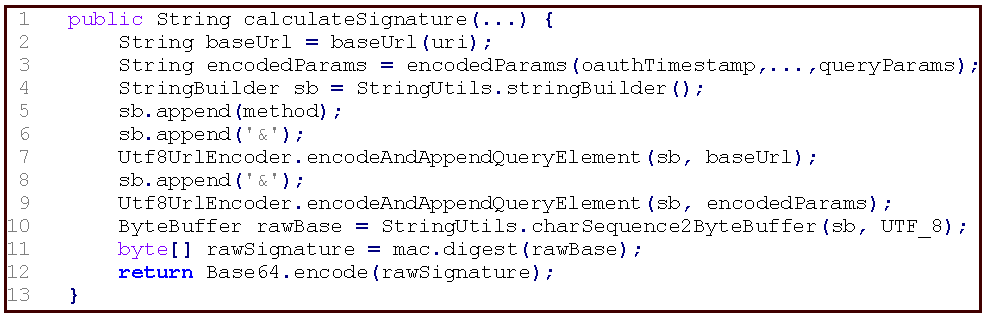
\includegraphics[width=\linewidth]{before.pdf}}
\vskip\baselineskip
\subfigure[函数抽取重构后函数]{\label{fig:after}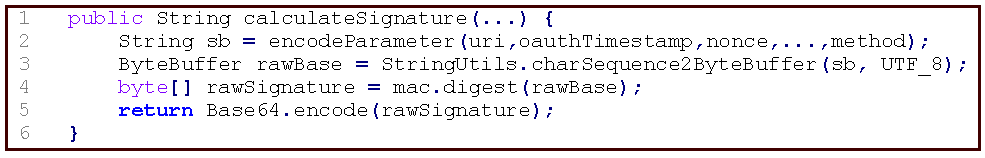
\includegraphics[width=\linewidth]{after.pdf}}
\vskip\baselineskip
\subfigure[新函数]{\label{fig:new}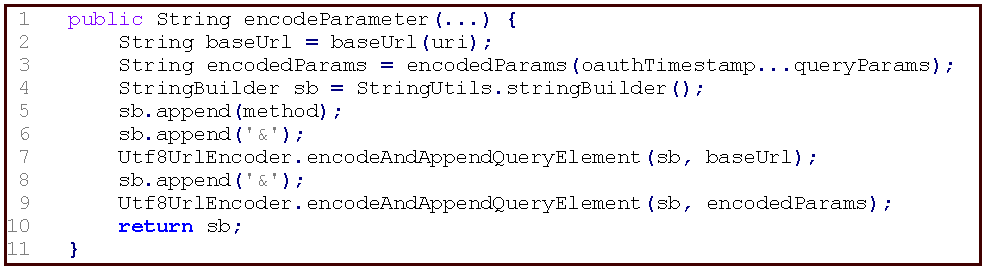
\includegraphics[width=\linewidth]{new_cropped.pdf}}
\caption{函数抽取重构示例}
\label{refactor-example}
\end{figure}

图~\ref{refactor-example}为来自AsyncHttpClient库\footnote{AsyncHttpClient为处理Java应用HTTP请求的代
码库:\url{https://github.com/AsyncHttpClient/async-http-client}}的一个简单的重构示例。图
~\ref{fig:before}为重构前的函数$calculateSignature()$,该函数的功能是计算HTTP签名。函数中第
2\textasciitilde9行实现了对参数进行编码的功能,并在接下来的版本中作为一个新的函数$encodeParameter()$
(图~\ref{fig:new})被提取出来。图~\ref{fig:after}为函数抽取重构后的函数,可以看到在第2行通过调用新
函数,保持函数的语义和功能不发生改变。

\begin{table}[!t]
\zihaowu
  \renewcommand{\arraystretch}{1.3}
  \caption{示例函数的函数抽取重构机会}
  \label{example_metrics}
  \centering
  \begin{tabular}{ccccc|ccccc}
  \toprule No.&Can&LCOM$_1$&LCOM$_2$&CPL &No.&Can&LCOM$_1$&LCOM$_2$&CPL\\ \midrule 1 &2-7 &8 &0 &6
   &9 &3-10 &6 &0 &6\\
   2 &2-8 &10 &0 &6 &10 &3-11 &13 &0 &6\\
   3 &\textbf{2-9} &11 &0 &6 &11 &3-12 &21 &0 &6\\
   4 &2-10 &13 &0 &6 &12 &4-9 &0 &0 &3\\
   5 &2-11 &28 &3 &6 &13 &4-10 &0 &0 &3\\
   6 &2-12 &36 &10 &6 &14 &5-7 &0 &0 &3\\
   7 &3-8 &4 &0 &6 &15 &5-8 &0 &0 &3\\
   8 &3-9 &5 &0 &6 &16 &5-9 &0 &0 &4\\
   \bottomrule
  \end{tabular}
\end{table}

为了模拟基于软件质量度量的函数抽取重构过程,表~\ref{example_metrics}中列出了函数$calculateSignature$
(如图~\ref{fig:before}所示)的16个候选函数抽取重构机会以及对应的软件质量度量。其中,Can为候选重构机
会,表~\ref{example_metrics}中使用起止代码行号来表示可被抽取的函数代码片段。表中列出了三种软件质量度
量方法,分别是函数内聚力缺乏度LCOM$_1$、LCOM$_2$和耦合度~\cite{yang2009identifying}。值得注意的是,
函数抽取重构中通常使用的LCOM$_1$和LCOM$_2$为描述函数体内部凝聚力的软件质量度量
~\cite{charalampidou2015size}。给定代码段$B$,$P$表示代码段中不共享任何变量的语句对的个数,$Q$为代码
段中存在共同变量的语句对的个数,则有$LCOM_1=P$。LCOM$_2$计算方式如下:
\begin{equation}\label{eq:lcom2}
      LCOM_2 = 
       \begin{cases}
             P-Q, & \textit{if}~P-Q\geq 0\\ 
  0, & elsewise,  
       \end{cases}
\end{equation}
不难看出,从函数体中抽取一个代码段,该代码段的LCOM$_1$和LCOM$_2$的值越低,表示其中不共享变量的语句对
越少,共享变量的语句对越多,此时代码段的内聚力越强。表~\ref{example_metrics}中的耦合度为抽取该代码段时
所需要的参数的个数~\cite{yang2009identifying},因此耦合度越低,表示此时需要的参数越少,代码段与重构后
的原函数相关性较低,更符合软件设计原则。为由于示例代码的结构较为简单,因此表~\ref{example_metrics}中
未列出关于复杂度的软件质量度量。根据图~\ref{refactor-example}可知,在列出的16个函数抽取重构机会中只
有第3个重构机会(第2\textasciitilde9行)代表了最终抽取的代码片段。从表~\ref{example_metrics}中可以看
出,第12\textasciitilde16个代码段具有更低的函数内聚力缺乏度和耦合度,因此根据软件质量度量更适合被抽
取出来组成新函数;相反,相比较其它候选重构机会,第3个代码段在三个度量标准上均未有明显的优势,因此很
难通过软件质量度量来解释该代码段在后续版本中被抽取出来的原因。

因此,利用特定的软件质量度量来推荐函数抽取重构机会存在一定的局限性:(1)虽然软件质量度量是为了评价
软件质量而设计的,然而现有的度量标准往往只考虑某一种特定的程序元素,例如LCOM只考虑了使用共同变量的语
句的个数,而其它与软件质量相关的程序元素,如函数调用、类型和包等并没有被考虑进去。(2)函数抽取的目
的并不仅仅是为了提高软件质量度量或是减少代码坏味,还包括缺陷修复、方便新功能的添加或者提高程序易读性
等很难被量化的目的。因此通过某个软件质量度量或预定义的公式来进行函数抽取重构推荐,容易导致推荐的不准
确性。本章提出通过学习开源软件仓库中的重构实例,挖掘函数抽取重构的原因,构建关于函数抽取重构的概率模
型来推荐函数抽取重构机会。

本章提出基于机器学习的函数抽取重构机会推荐模型,通过提取一组结构特征和一组功能特征来对候选函数抽取重
构机会进行表示。具体来说,在特征提取算法中,提取了一组与函数和候选代码片段的复杂度相关的结构特征,以
及一组与内聚度和耦合度相关的功能特征。与传统的软件质量度量不同,该模型将软件质量相关的特征用一系列程
序元素来表示,包括与代码功能相关的变量使用、函数调用和包等。通过融合多种软件质量概念和程序元素,将函
数抽取重构机会表示为可供学习的特征序列。通过从开源软件仓库中挖掘真实存在的函数抽取重构实例,模型可以
从中学习到关于函数抽取重构的概率模型。给定一个新的函数体,该模型生成的候选函数抽取重构机会,并为每个
合法的重构机会分配一个概率,表示该重构机会为使用者所采纳的可能性,并按照概率由高至低进行推荐。

\subsection{相关工作}
函数抽取重构推荐主要分为两个步骤:给定待重构的函数体,首先识别可以被抽取的代码段作为候选重构机会,然
后根据某种特定的方式将候选重构机会进行排序,并按序推荐给软件维护人员。因此,根据函数抽取重构的过程,
可以将关于函数抽取重构推荐的研究分为两个部分,分别是函数抽取重构机会识别和排序。本节从上述两个角度来总结和分析当前主流的函数抽取重构机会推荐方法。

\subsubsection{函数抽取重构机会识别}

函数抽取重构机会识别指的是识别函数体中可以抽取的代码从而组成一个新的函数的代码,其本质是对函数体进行
拆分。目前关于识别函数抽取重构机会的研究主要分为基于程序语法和语义两种。

基于程序语法的函数抽取重构机会识别,主要通过程序切片的方式保证程序语法的正确性。Maruyama等人
~\cite{maruyama2001automated}首次提出使用程序切片来识别函数抽取重构机会,提出了个基于基本代码块的切
片方法对程序的控制流图进行切片。虽然该方法利用基本块来限制程序切片的范围,但由于其无法从语法上保证抽
取代码段前后程序的行为保持一致,因此其实用性受到了限制。为了保证函数抽取重构不会使程序行为发生改变,
Tsantalis和Chatzigeorgious~\cite{tsantalis2011identification}针对给定变量和对象,通过计算程序切片得
到所有可能改变变量的值或对象的状态的可执行切片。通过对程序切片的完全计算,该方法能够对给定的切片要求
(如某个特定的变量),在提取出所有与指定要求相关的代码片段的同时不改变原来的程序行为。

除了程序切片外,Yang等人~\cite{yang2009identifying}提出了针对规模较大的函数(``长函数''代码坏味)的
函数拆分方法,该方法根据函数的层次结构(如空行、分支和循环等)将长函数拆分成多个代码片段作为函数抽取
重构机会。Meananeatra~\cite{meananeatra2011using}等人定义了一组关于程序控制流和数据流的布尔表达式来
筛选被抽取的代码段,从而保证程序行为不变。例如,通过限制变量的定义和使用关系,确保变量在使用前已经被
定义,该方法可以过滤掉只包含某个变量的使用而不包含该变量定义的代码片段。Silva等人
~\cite{silva:ICPC14,silva:CoRR15}提出了基于代码块的函数抽取重构机会生成算法,将函数体表示为具有层次
结构的代码块的组合,每个代码块由顺序执行的子代码块组成。针对每个代码块,其中连续的子代码块组成一个候
选函数抽取重构机会。通过这样的方式,该算法能够生成所有能够顺序执行的代码片段,最终通过规则筛选出所有
合法的函数抽取重构机会。

基于程序语法的函数抽取重构机会识别,通常只能保证函数抽取重构后程序的语义和功能不发生改变,但仍然依赖
软件维护人员判断如何选取函数抽取重构机会(或指定切片条件)。根据``一个功能原则
''~\cite{martin2003agile}(Single Responsibility Principle,SRP),软件系统内的每个函数应该完成一个明确
的、特别的功能。基于这个原则,Charalampidou等人~\cite{charalampidou2016identifying}认为应该识别可能
完成某个特定功能的代码片段进行函数抽取重构。具体来说,他们认为在距离相近的有共同变量或函数调用的代码
语句在完成同一个功能,因此将这些语句视为一簇;通过合并重叠的小簇形成大簇,然后将每个大簇作为一个候选
重构机会。通过这种方法,他们认为能够识别所有可能在执行同一个程序功能的代码片段。然而,该方法在限制代
码之间距离的同时也限制了被抽取的代码片段的规模。例如,在代码片段中位置比较靠前的变量声明语句,由于距
离变量的使用存在一定距离,因此经常容易被忽略。除此以外,该方法在考虑代码功能的时候只考虑了变量和函数
调用,而没有考虑其它和代码功能相关的程序元素,如类型、包等。

\subsubsection{函数抽取重构机会评价}

函数抽取重构是从给定函数体中抽取代码片段组成新函数并调用的过程。然而,能够抽取并保持程序行为不变的代
码片段通常有很多,尤其当函数规模变大时,其函数抽取重构机会的数量往往呈指数级上升。为了提高软件维护的
效率,部分研究对函数抽取重构机会进行排序,然后按序将候选重构机会推荐给使用者。

目前大部分关于函数抽取重构机会推荐的研究是根据函数级软件质量度量来对候选重构机会进行排序。软件质量度
量为从质量角度对软件系统的度量,其中与函数抽取重构相关的主要有复杂度、内聚度和耦合度等。根据SRP原
则,理想的函数抽取重构可以降低原函数的复杂度,使原函数和新函数内聚度尽可能高、耦合度尽可能低。

具体来说,基于复杂度的概念,部分研究使用函数复杂度(Method Complexity,MCX)来对函数抽取重构机会进行
排序~\cite{meananeatra2011using, yang2009identifying},倾向于推荐可以使函数复杂度尽可能小的重构机
会。基于内聚度的概念,部分研究使用函数内聚缺乏度(Lack of Cohesion of Method,LCOM)来评估函数抽取重
构对软件质量的改进程度,优先推荐让原函数和新函数的函数内聚缺乏度尽可能低的函数抽取重构机会
~\cite{meananeatra2011using, charalampidou2016identifying}。基于耦合度的概念,部分研究者提出优先推荐
尽可能独立的代码片段,使得重构之后原函数和新函数相关性尽可能小
~\cite{yang2009identifying,silva:ICPC14,silva:CoRR15},例如可以通过计算函数抽取时新函数所需要的参数
的数量来评估新函数对原函数的依赖性~\cite{yang2009identifying}。

与基于软件质量度量的方法不同,考虑到函数抽取重构原因的多样性~\cite{silva2016we}和软件质量度量的局限
性,本章提出构建关于函数抽取重构的概率模型,挖掘开源软件仓库中学习的重构实例,从中学习如何进行函数抽
取重构;除此以外,开发了``生成-排序''的推荐系统,为给定函数体生成所有合法的函数抽取重构机会,然后使
用训练好的模型为每个重构机会分配一个概率作为分数,按照分数由高至低进行推荐。与本章工作最相近的是
Silva等人的JExtract~\cite{silva:ICPC14,silva:CoRR15},该方法与本章方法的共同点是在识别函数抽取重构机
会的阶段不对重构机会进行筛选,而是依赖于后续的排序方法为使用者推荐重构机会;最大的区别是JExtract中的
排序算法假设被抽取的代码片段应该尽可能独立,因此JExtract计算待抽取代码与剩余代码之间的结构依赖性,推
荐尽可能独立的代码片段进行函数抽取重构。然而,软件维护人员进行函数抽取的原因多种多样
~\cite{silva2016we},只考虑结构依赖性作为函数抽取的原因在某些情况下存在一定的局限性。

\section{研究方法}
软件重构是完善性软件维护的重要手段。针对最常见的软件重构类型之一--函数抽取重构,本文提出了基于梯度上
升决策树的函数抽取重构机会推荐方法,并开发了基于Eclipse的插件GEMS。本节首先介绍了方法的基本框架,然
后提出了针对函数抽取重构实例的特征提取算法,接着阐述了本文使用的梯度上升决策树和逻辑斯特回归融合模
型,最后针对预测阶段给定函数体,阐述了基于代码块的候选函数抽取重构机会生成的方法,并描述了模型预测和
排序的过程。

\subsection{基本框架}
基于梯度上升决策树的函数抽取重构机会推荐方法,主要包括模型训练和重构推荐两个阶段。

在训练阶段,为了挖掘函数抽取重构的原因,本章提出基于数据驱动的函数抽取重构机会推荐,通过对比开源软件
仓库中两个相邻的提交版本,收集函数抽取重构实例作为样本。然后针对训练样本集中的函数抽取重构实例进行特
征提取,根据特征提取算法将其表示为一个特征向量(feature vector)。在将训练样本通过特征提取算法表示完
成后,利用基于梯度上升决策树和逻辑斯特回归的融合模型进行训练。

在推荐阶段,给定函数体,首先基于代码块的函数抽取重构机会生成算法,将所有在一个代码块内的连续子块作为
可能的函数抽取重构机会。然后筛选函数抽取重构机会。由于基于代码块的重构机会生成算法可能生成破坏程序语
义和功能的重构机会,因此使用基于规则的方法对函数抽取重构机会进行筛选,得到由所有合法重构机会组成的集
合。最后对函数抽取重构机会进行预测和排序推荐。针对集合中的每一个函数抽取重构机会,使用训练好的模型预
测其为训练样本中正例的概率,并根据概率由高至低进行排序,按序推荐给使用者。

值得注意的是,虽然本章方法需要一定的训练时间,但由于该训练过程是离线的,在训练完成后可以直接部署在集
成开发环境中,由使用者指定需要重构的函数,使用训练好的参数进行重构推荐,因此效率较高。

\subsection{相关定义与特征提取算法}
\subsubsection{相关定义}

\begin{Definition}
  函数抽取重构机会。给定函数$m$,$c$为函数$m$中由连续语句组成的代码片段,若代码片段$c$能够被抽取
  出来组成一个新的函数,并在原函数$M$中以同样的方式调用,使原函数$m$的功能和语义保持不变,则代码片段
  $c$为函数$m$的一个函数抽取重构机会。
\end{Definition}

\begin{Definition}
  函数-重构机会对。函数$m$和其中一个函数抽取重构机会$c$组成了一个函数-重构机会对$p$,记为$p=(m,c)$。
\end{Definition}

\begin{Definition}
  函数抽取重构实例。给定函数$m$,若其中的一个函数抽取重构机会$c$在后续的版本中被提取出来进行函数抽取
  重构,则函数$m$和$c$组成一个函数抽取重构实例$r$,记为$r=(m,c)$。
\end{Definition}

本文通过比较开源软件仓库中的相邻版本得到的真实的函数抽取重构实例集$\mathcal R$。给定训练样本集
$\mathcal D$,其中第$i$个样本记为$\mathcal D^{(i)}=(x^{(i)},y^{(i)})$,$x^{(i)}$表示样本数据,为一个
函数-重构机会对,即$x^{(i)}=p^{(i)}=(m^{(i)},c^{(i)})$;$y^{(i)}$表示样本的标签,即该函数-机会对是否
为函数抽取重构实例。因此样本标签$y^{(i)}$可以表示为:
\begin{equation}
   y^{(i)} = 
       \begin{cases}
             1, & \textit{if}~p^{(i)}\in \mathcal D\\ 
  0, & elsewise,  
       \end{cases}
\end{equation}

为了学习关于函数抽取重构的概率模型,首先对样本$D^{(i)}\in\mathcal D$的输入数据$x^{(i)}$表示成特征向
量$x^{(i)}=(x^{(i)}_1,x^{(i)}_2,...,x^{(i)}_n,)$,其中$n$为特征的个数。针对每个函数-重构机会对,通过静态
分析提取关于结构和功能的两组特征。尽管本文方法不是为了推荐满足某个特定软件质量度量的函数抽取重构机
会,但根据SRP原则,本文的特征提取算法中融合了包括复杂度、内聚度和耦合度在内的软件质量因素,并考虑了
多种程序元素。值得注意的是,虽然在特定情况下函数抽取也被用来防止代码重复,但针对以避免代码重复为目的
的函数抽取重构并不在本文的研究范围内,因为在研究中通常使用代码克隆检测技术来避免代码重复
~\cite{bellon2007comparison}。

\subsubsection{结构特征}

给定由函数$m$和重构机会$c$组成的函数-重构机会对$p$,首先根据函数抽取重构机会将函数$m$分为两部分:待抽取
的代码片段和剩余代码。对每部分代码$g$,GEMS提取其控制流图$graph(g)$,并计算其函数复杂度(MCX):
\begin{equation}
   MCX(g) = E(g) - N(g) + 2P(g)
\end{equation}
其中,$E(g)$表示控制流图$graph(g)$中边的个数,$N(g)$表示$graph(g)$中节点的个数,$P(g)$表示$graph(g)$
中连通分支的个数。通过这样的方式,计算出待抽取代码片段和剩余代码的函数复杂度。除软件度量外,GEMS还通
过简单的程序分析提取了其它与代码复杂度相关的特征。如根据控制流语句得到代码片段中各种代码结构(如分支
结构、循环结构)的数量;根据变量、类型、函数调用等,得到关于代码片段中各种程序元素的数量。本文从直观
上认为使用更多的变量、类型、循环等程序元素的代码片段通常更加复杂,因此易读性和易理解性更低。

值得注意的是,GEMS虽然提取了一组跟复杂度相关的结构特征对样本进行表示,但并没有假设其中的每个特征均与
模型预测结果相关,特征与是否进行函数抽取重构之间的关系仍需要依赖模型训练学习得到。换言之,提取的特征
只是可能与函数抽取重构相关的特征,但不能保证不存在``冗余特征''。关于特征对模型的影响和特征选择的分
析,本文会在~\ref{discuss}通过实验进一步讨论和分析。

除此以外,之前的研究通过设置阈值来限制被抽取代码的规模
~\cite{silva:ICPC14,charalampidou2016identifying}。与之前的研究不同,GEMS通过计算被抽取代码行数占总
代码行数的百分比作为特征,让模型学习函数抽取重构机会与代码规模的关系。通过这样的方式,GEMS提取被抽取
的代码片段的规模作为特征,让模型在推荐阶段能够过滤掉抽取过量或极少量代码的函数抽取重构机会。例如,通
过实验发现,大部分只抽取一行代码和几乎抽取整个函数体的重构机会被分配到较低的概率,因此很少被推荐给使
用者。

\subsubsection{功能特征}

由于函数抽取重构的过程是将原函数中的代码段抽取出来组成一个新函数,而同时根据SRP原则,每个函数应该完
成一个独立的、明确的函数功能,因此,虽然函数抽取重构的原因较为复杂和多样,但通常被抽取的代码段在功能
上应该相对独立。另一方面,调查发现,函数抽取重构的主要目的之一将原函数功能拆分成多个子功能,每个子功
能完成一个相对独立的功能,从而提高软件系统的易理解性和可维护性~\cite{silva2016we}。因此,除了结构特
征外,GEMS还提取了一组与功能相关的特征。

给定函数-重构机会对$p=(m,c)$,GEMS提取了一组功能特征来判断函数抽取重构机会$c$是否选择一个独立的、内
聚的、具有某个函数子功能的代码段。具体来说,对代码段功能特征的提取主要分为两步:
\begin{itemize}
  \item 基于耦合度的概念,提取函数抽取重构机会$c$中可能完成的、剩余代码$m-c$中所未提供的函数
  子功能$q$;
  \item 基于内聚度的概念,计算函数抽取重构机会$c$所选择的代码段对函数子功能$q$的凝聚度,即被抽取的代
  码对子功能$q$的投入程度。
\end{itemize}

具体而言,对于函数-重构机会对$p=(m,c)$中的待抽取代码段,GEMS首先提取其可能独立执行的某个函数子功能,
具体方式是寻找只出现或主要出现在待抽取代码段中的程序元素。传统的软件质量度量只考虑特定的程序元素作为
评价软件质量的方法,例如LCOM$2$中只考虑不同语句对变量的使用来推断它们的相关性。与传统的软件质量度量
不同,本文考虑了与程序功能相关的变量、函数调用、类型、包四种程序元素类型。之所以在特征提取阶段考虑多
种程序元素,是因为除了变量外,完成一个功能通常还涉及到类型、函数调用、代码库等多种程序元素
~\cite{martin2003agile},而部分程序元素可能比变量本身更能体现代码所执行的功能。对每种程序元素类型,
本文首先寻找该类别中在待抽取代码段和剩余代码段中出现频率相差最大的具体程序元素,作为可能代表待抽取代
码的独立子功能的程序元素。然后,在从待抽取代码段中提取出可能代表其独特子功能的程序元素后,接下来就是
计算该代码段对函数子功能的投入程度。与传统的软件质量度量不同,本文在对代码段对函数子功能的投入程度时
综合考虑了多种程序元素,因此对于上一步骤中提取出来的最有可能代表代码段独特子功能的每个程序元素,本文通过
计算代码段中使用到该程序元素的语句占待抽取代码段语句的比例,来计算代码段对该独特子功能的投入程度。



\begin{algorithm}[H]
\caption{功能特征提取算法}\label{alg:feature}
\KwIn{函数$m$,待抽取代码片段$b$,程序元素类型序列$W$;}
\KwOut{功能特征向量$f$;}
获取函数$m$中的所有语句$S_m$;\\
获取代码片段$b$中的所有语句$S_b$;\\
\For {$w$ in $W$} {
  //对每种程序元素类型$w$进行计算\\
  获取待抽取代码段$b$中的所有类型为$w$的程序元素,得到序列$E_w$;\\
  \For {$e$ in $E_w$} {
    统计程序元素$e$在函数$m$中出现的频率$freq_m$;\\
    统计程序元素$e$在代码段$b$中出现的频率$freq_b$;\\
    计算$ratio_e = freq_b/freq_m$;\\
  }
  选择$E_w$中$ratio$最大的程序元素$e^*$;\\
  令$cp_w = ratio_{e^*}$;\\
  计算代码段$b$的代码行数$loc = getLOC(b)$;\\
  初始化$count = 0$;\\
  \For {$s$ in $S_b$} {
    //对代码段$b$中的每个语句\\
    \If {$e^*$ in $s$} {
      更新$count = count + 1$;\\
    }
  }
  计算$ch_w = count/loc$;\\
  将$cp_w$和$ch_w$设置为程序元素$w$的两个功能特征。\\
}
\end{algorithm}

算法~\ref{alg:feature}描述了提取功能特征的过程。给定函数-重构机会对$p=(m,c)$,其中$m$为原函数,$c$为
函数重构机会,$b$为该重构机会中待抽取的代码片段,GEMS首先获取$m$和$b$中的语句,得到集合$S_m$和$S_b$
(第1\textasciitilde2行)。然后,对于程序元素类型集合$W$中的每种程序元素类型$w$,首先基于耦合度的概
念,提取该类型中最独特的程序元素$e^*$(第6\textasciitilde14行);然后基于内聚度的概念,计算待抽取代
码中该程序元素被使用的程度(第15\textasciitilde23行);最后将这两类特征分别放到特征向量中(第24
行)。


其中,程序元素类型$W$主要包括四种:变量、类型、函数调用和Java包。对于每一种程序元素类型$w$,首先获取
待抽取代码$b$中所有该类型的程序元素$E_w$(第5行);然后针对其中的每种程序元素$e$,分别计算该元素在函
数$m$和代码段$b$中出现的频率$freq_m$和$freq_b$(第7\textasciitilde8行),并计算频率的比例$ratio_e$
(第9行);通过选择具有最大$ratio$的程序元素,得到该类型中最主要在待抽取代码中出现的程序元素$e^*$
(第11行)。以Java包为例,如果某个Java包只在待抽取代码中被使用,则该Java包对应的$ratio$为1,此时该类
型的$cp$也为1(第12行)。通过这种方式,提取到可能代表待抽取代码段独特子功能的4种程序元素。需要声明的
是,为了容易理解,在算法~\ref{alg:feature}中为每种类型只选择了一个程序元素,而在实际模型中对每类程序
元素选择$ratio$最大的两个元素计算$cp$作为耦合度相关特征。最后对上述可能代表程序子功能的程序元素,分
别计算在待抽取代码段$b$中使用的程度(第13\textasciitilde21行),若某个程序元素出现在代码段$b$中的每
个语句中,则此时对应的$ch$为1,说明此时待抽取代码段的内聚力较高。最后对每类程序元素分别计算得到$cp$
和$ch$后,将其作为功能特征向量返回。通过这种方式,针对给定函数和待抽取代码段,该算法能够抽取出代码段
可能完成的独特的函数子功能,从而通过特征提取将内聚度和耦合度的概念融入到模型中。

\subsection{梯度上升决策树}
给定训练数据集$\mathcal D$中的第$i$个样本${\mathcal D}^{(i)}=(x^{(i)},y^{(i)})$,通过特征提取将$x^{(i)}$
其表示为$x^{(i)}=\{x_1^{(i)},x_2^{(i)},...,x_n^{(i)}\}$;$y^{(i)}$为第$i$个样本的类别,$y^{(i)}=1$表
示第$i$个样本为正样本,$y^{(i)}=0$表示第$i$个样本为负样本。在将训练数据集表示为特征向量和标签后,构
建基于梯度上升决策树的二分类模型,通过使用$Logloss$作为损失函数,拟合样本为正样本的概率;在推荐阶
段,使用训练完成的模型为给定函数抽取重构机会预测其为正样本的概率,并按照概率由高至低推荐函数抽取重构
机会。

首先简单阐述基于梯度上升决策树的原理。梯度上升决策树为基于多个弱学习器的融合模型,由于梯度上升决策
树的目标是为给定样本预测一个连续值,因此其使用的弱学习器为回归树。梯度上升决策树的优点在于:(1)通
过融合多个弱学习器,得到对性能的显著提升;(2)在训练阶段,可以保持现有模型不变,通过增加新的弱学习
器(决策树),提高模型的表现,使用较为灵活;(3)能够发现有效的特征组合。具体来说,本文使用CART回归
树作为弱学习器,在节点分裂的时候使用最小均方差(Mean Squared Error,MSE)作为分裂准则,选择使每个分
支的均方差之和最小的条件作为节点分裂的条件。

本文使用的基于梯度上升决策树的二分类模型,因此选用$Logloss$作为损失函数:
\begin{eqnarray}
  Loss(y^{(i)},F_k(x^{(i)})) = -(y^{(i)}logp^{(i)} + (1-y^{(i)})log(1-p^{(i)})),
\end{eqnarray}\label{logloss}
其中$F_k(x^{(i)})$表示$x^{(i)}$在以前$k$棵树作为模型时的预测结果,根据罗基斯特方程,$p^{(i)}$为
$x^{(i)}$为正样本的概率:
\begin{eqnarray}
  p^{(i)} = \frac{1}{1 + e^{-F_k(x^{(i)})}}.
\end{eqnarray}
梯度上升决策树通过每次新增一个树$F_k$来拟合损失函数的负梯度在当前模型$F_{k-1}$的取值。

\subsection{函数抽取重构机会推荐}
在推荐阶段,对于给定函数,首先生成所有可能的函数抽取重构机会,然后通过基于规则的方法过滤掉可能改变程
序行为的代码片段,得到所有合法的函数抽取重构机会后,使用训练好的梯度上升决策树模型为合法重构机会分配
概率,并按照概率由高至低推荐给用户。

\subsubsection{函数抽取重构机会生成}
本文的函数抽取对象为连续语句构成的代码片段,因此给定函数,需要在不破坏程序语法的前提下,生成所有可能
的函数抽取重构机会,通过分析函数的控制流结构,生成代码结构树,并通过对代码结构树的遍历得到所有可能的
函数抽取重构机会。

\begin{figure} 
  \centering 
  \begin{minipage}[c]{0.5\textwidth} 
    \centering 
    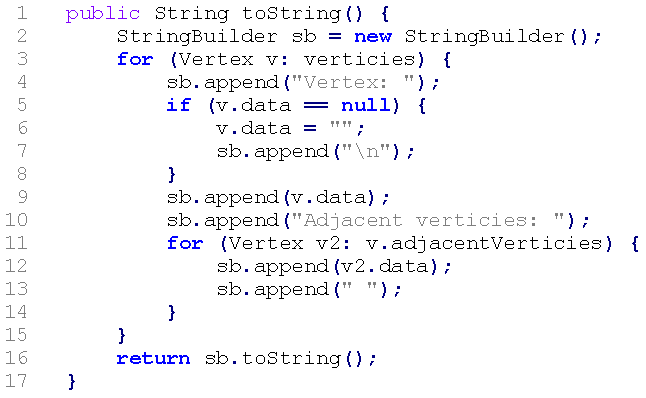
\includegraphics[width=3in]{block.pdf} 
  \end{minipage}% 
  \begin{minipage}[r]{0.5\textwidth} 
    \centering 
    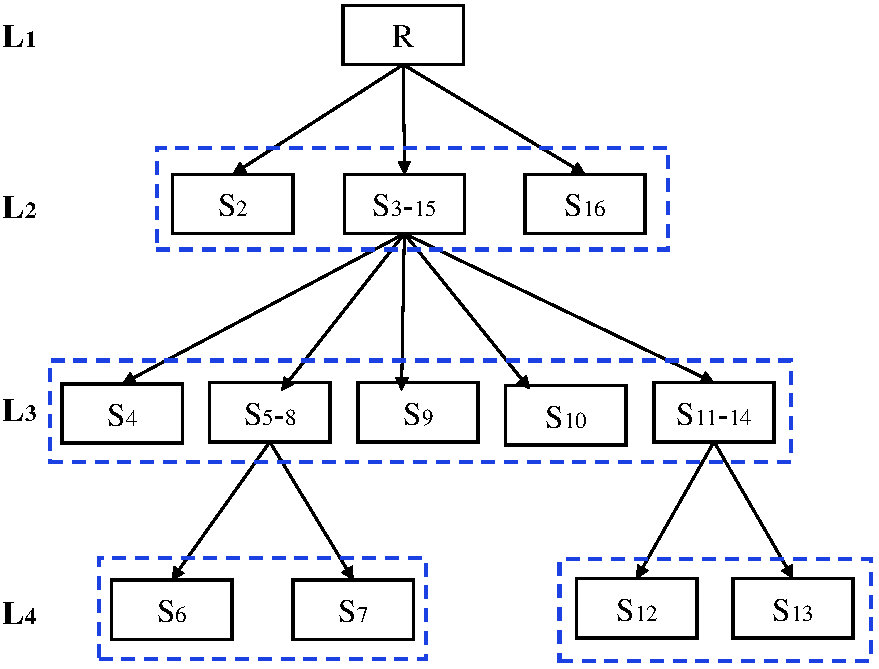
\includegraphics[width=2in]{block_structure.pdf} 
  \end{minipage} 
\caption{示例代码的结构表示}
\label{block-example}
\end{figure}

图~\ref{block-example}为示例代码及其代码结构树,其中代码结构树中的$S_j$指代的是示例代码的第$j$行代
码。可以看到,示例代码的代码结构树高度为4,其中包括根节点在内,共有4个非叶子结点,分别为$R$、
$S_{3-15}$、$S_{5-8}$和$S_{11-14}$,每个非叶子节点表示代码内部的一个控制结构,在图
~\ref{block-example}中用蓝色虚线框表示。以根节点$R$为例,$R$的3个子节点分别为$S_2$、$S_{3-15}$和
$S_{16}$,表示函数$toString()$一共包括3条语句,依次为语句$S_2$、$for$循环语句$S_{3-15}$和语句
$S_{16}$。通过对代码结构树进行遍历,针对树中的每个非叶子结点,生成由连续子节点组成的代码片段,得到所
有可能的函数抽取重构机会。

以根节点为例,根节点的子节点从左到右依次为$Child(R)=\{S_2,S_{3-15},S_{16}\}$。由于根节点共有3个子节
点,因此可以依次生成长度为1的连续语句:$\{\{S_2\},\{S_{3-15}\},\{S_{16}\}\}$、长度为2的连续语句
$\{\{S_2,S_{3-15}\},\{S_{3-15},S_{16}\}\}$和长度为3的连续语句:$\{\{S_2,S_{3-15},S_{16}\}\}$。最后可
以得到,根据代码块$B_1$生成的代码片段有
$cf(B_1)=\{\{S_2\},\{S_{3-15}\},\{S_{16}\},\{S_2,S_{3-15}\},\{S_{3-15},S_{16}\},\{S_2,S_{3-15},S_{16}\}\}$。
通过同样的方式,遍历4个非叶子结点后一共得到27个由连续语句组成的代码片段作为潜在的函数抽取重构机会。
需要注意的是,对于非叶子结点而言,其子节点可以是普通语句或是结构语句(如分支、循环等),例如根节点
$R$的第二个子节点为一个$for$循环语句。

\subsubsection{函数抽取重构机会筛选}
由于函数抽取重构的前提是不改变程序的语义和行为,因此为了避免重构后发生编译错误,需要对基于代码块生成的所有可能的函数抽取重构机会进行筛选,过滤掉以下情况:
\begin{itemize}
  \item 根据Java编程语言的要求,每个函数不能有超过一个返回值,因此要过滤掉那些在抽取函数后需要返回不
  止一个值到原函数的函数抽取重构机会;
  \item 由于类型的声明和使用应该在一个代码块中,因此要过滤掉导致类型的声明和使用被分开的函数抽取重构
  机会,例如某个类型的声明语句被抽取而对于该类型的使用仍然留在原函数中;
  \item 如果被抽取的代码片段中含有$continue$、$break$或者$case$等语句,然而却不包含与其相配套的代码
  结构,则该函数抽取重构机会被视作非法的,应当被过滤掉。
\end{itemize}

\subsubsection{预测与排序}
在推荐阶段,给定函数$m$后,为其生成所有合法的函数抽取重构机会$P(m)$,根据特征提取算法,为每个函数
抽取重构机会$p\in P(m)$提取一个特征向量$f(p)$作为输入数据$x(p)$,使用训练好的模型参数预测该特征向量
的输出$y(p)$,$y(p)$表示函数抽取重构机会$p$为正例的概率。在对每个合法函数抽取重构机会分配一个概率
后,按照概率由高至低将函数抽取重构机会推荐给用户。需要注意的是,在实际应用中用户很难看完所有的重构机
会再进行选择,因此在使用中通常只推荐排名最高的若干个函数抽取重构机会。

\section{实验设计}
在基于梯度上升决策树的函数抽取重构机会推荐模型的基础上,开发了基于Eclipse的开源工具GEMS\footnote{http://www.comp.nus.edu.sg/~specmine/gems}。为了评估方法的有效性,通过在5个开源软件上进行
实验,对比评估了GEMS与其它3种当前流行的函数抽取重构机会推荐方法,证明了本文的有效性。除此以外,
还设计了关于模型选择和特征重要性的实验,并对实验结果进行了讨论和分析。

\subsection{对比方法与实验对象}
为了评估本章方法的有效性,与3个当前流行的函数抽取重构机会推荐工具进行对比实验,这三个工具分别是:
\begin{itemize}
  \item JExtract~\cite{silva:ICPC14,silva:CoRR15},该工具同样也是一个``生成-排序''系统,与本章方法的
区别是JExtract使用自定义的函数为每个函数抽取重构机会打分,而GEMS通过构建概率模型学习如何进行函数抽取
重构。
  \item SEMI~\cite{charalampidou2016identifying},该方法通过识别连续的相关的代码语句作为候选函数抽取
机会,并按照软件质量度量LCOM$_2$的高低进行排序并推荐。
  \item JDeodorant~\cite{tsantalis2011identification},该工具通过计算程序切片得到所有可能改变变量的
  值或对象的状态的可执行切片作为候选函数抽取重构机会进行推荐。
\end{itemize}

本章的实验对象为5个开源软件,分别是JHotDraw、Junit、MyWebMarket、SelfPlanner和WikiDev。其中
JHotDraw、Junit和MyWebMarket为文献~\cite{silva:ICPC14}中用来证明JExtract有效性的实验对象,
SelfPlanner和WikiDev与文献~\cite{tsantalis2011identification}中用来证明JDeodorant有效性的实验对象相
同,而文献~\cite{charalampidou2016identifying}使用了这5个软件系统来评估SEMI的有效性。表
~\ref{benchmark}为这5个开源软件系统的统计信息。可以看到,在这5个开源软件中的共有130个函数存在函数抽
取重构操作,而实验的目标是为这130个函数中准确识别出155个函数抽取重构机会。需要注意的是,用来评估方法
有效性的这155个函数抽取重构均来自于专家或者软件开发者的意见,因此本章实验中将其作为基准集来验证方法
有效性。

\begin{table}[!t]
\zihaowu
  \renewcommand{\arraystretch}{1.3}
  % if using array.sty, it might be a good idea to tweak the value of
  % \extrarowheight as needed to properly center the text within the cells
  \caption{实验对象统计信息}
  \label{benchmark}
  \centering
  \begin{tabular}{ccc}
  \toprule 
  程序名 &函数数量 &函数抽取重构数量.\\ \midrule
  JHotDraw &56 &56 \\ 
  Junit &25 &25 \\ 
  MyWebMarket &23 &35 \\ 
  SelfPlanner &12 &13 \\ 
  Wikidev &14 &26 \\ \midrule
  Total &130 &155 \\ 
  \bottomrule
  \end{tabular}
  \end{table}

\subsection{训练数据收集}
为了训练函数抽取重构的概率模型,首先需要收集正负样本作为训练数据集。本文收集了以下两组训练数据集:

\textbf{函数抽取重构实例。}实验中的真实数据集来自于GitHub上广受欢迎的开源软件系统,利用
RefactoringMiner工具~\cite{tsantalis2013multidimensional}比较两个相邻的版本,收集在原函数中存在的、
在后一个版本中被抽取出来作为新函数的代码片段,得到可能的函数抽取重构实例。由于RefactoringMiner不能完
全正确,因此通过人工检查过滤掉程序语义不完全一样的样本,最后得到267个真实的函数抽取重构实例作为训练
样本集中的正例。训练样本集中的负例来自于对未被函数抽取重构的函数随机生成并通过合法性筛选的重构机会。
由于给定任意函数的函数抽取重构机会的数量往往较大(如本文实验中为5个开源软件生成了7628个重构机会),
然而其中应该被实施的函数抽取重构实例通常较少(如实验中只有155个函数抽取重构实例),因此本文假设随机
生成的重构机会大概率不应该被实施,因此将它们作为负样本。

\textbf{数据集扩充方法。} 由于收集真实的函数抽取重构实例需要进行人工筛查,其时间和人力的成本较高,因
此收集到的真实训练数据集规模较小。为了扩大训练数据集规模,在实验中内联只被调用过一次的函数,将其与调
用函数合并构成一个函数抽取重构样本。基于变异测试的思想,该方法假设被合并的代码片段应该重新被抽取出
来。通过对软件系统设计良好的开源软件以上述方法扩充训练数据集,最后一共得到5598个正样本,并生成同等规
模的负样本,构成扩充训练样本集。
  
在接下来的实验中,分别利用这两个训练数据集单独进行实验,并对实验结果进行比较分析。为了确保实验的可重
复性,所有的训练数据集、实验数据集以及GEMS工具和源代码均已放到网站上。需要注意的是,由于GEMS和其它三
种函数抽取重构推荐工具都只针对待重构函数进行分析,输入数据不包括其它函数或文件,因此虽然代码复用是函
数抽取重构的原因之一,但这些方法均不考虑这种原因。可通过代码克隆检测来寻找重复的代码,并进行函数抽取
重构。

\subsection{评估方法}
\subsubsection{正确性与容忍度}\label{tol}
给定函数$m$和$m$的一个函数抽取重构机会$p$,若$p$与实验数据集中的函数抽取重构操作完全匹配,则认为该函
数抽取重构机会是正确的。与之前的研究一样\cite{charalampidou2016identifying},在实验评估中引入容忍度
(tolerance)的概念,即在判断函数抽取重构机会是否正确的时候,容忍在一定范围以内的误差。一方面,软件
重构本身具有一定的主观性,而在待抽取代码段边界上的代码定位可能较为模糊,不是很明确地属于某个子功能;
另一方面,对于规模较大的函数,即使是在一定误差范围以内的函数抽取重构机会推荐也能够提高对程序的理解和
维护效率。具体来说,实验中分别使用$1\%$, $2\%$ and $3\%$作为容忍度$t$的阈值。以LOC为100的函数为例,
$t=1\%$意味着将误差在1行以内的函数抽取重构机会在评估时认为是正确的。

\subsubsection{评估指标}
在评估方法有效性时,按照之前的研究,使用三个评估指标来评估方法的性能和效率,分别是精确率、召回率和F
值。其中,精确率指的是所有被推荐的函数抽取重构机会中正确函数抽取重构机会所占的百分比;召回率指的是被
寻回的函数抽取重构机会占总数的百分比;$F-measure$是一个对精确率和召回率的加权调和平均:
\begin{eqnarray}
  F-measure = \frac{2 \times precision \times recall}{precision + recall} \times 100\%,
\end{eqnarray}
\label{f1}
其中,$Precision$为精确率,$Recall$为召回率。最后,根据容忍度$1\%$, $2\%$ and $3\%$分别计算上述三个指标在实验数据集上的结果,比较分析包括本章方法在内的4个函数抽取重构机会推荐工具。

\subsubsection{参数设置}\label{canshu}
为了有效评估方法的性能,将本章方法与其它三种工具进行对比实验。与最终部署到Eclipse上的插件GEMS相同,
在第~\ref{RQ1}节中呈现的是使用的是梯度上升决策树在扩展训练数据集上训练的模型进行推荐的结果(用
$GEMS^{GB}$表示)。为了实验的公平性,JExtract根据开发者的建议,将推荐的函数抽取重构机会的最小LOC设置为
2;SEMI和JDeodorant同样根据文献中推荐的方法进行设置。

\section{实验结果与分析}
本节首先比较了基于梯度上升决策树的函数抽取重构机会推荐方法与其它主流方法的准确性(第~\ref{RQ1}节),
然后在第~\ref{RQ2}节中比较了使用两组训练数据集进行训练所学习到的模型的性能,在第~\ref{RQ3}节中通过实
验比较了训练所使用的分类模型对实验结果的影响,最后通过在长函数上的实验分析并讨论了本文方法的优点和不
足(第~\ref{RQ4}节)。

\subsection{函数抽取重构机会推荐工具比较}\label{RQ1}
在四种工具中,GEMS和JExtract为``生成-排序''工具,因此给定130个待重构函数,GEMS和JExtract首先生成尽可
能多的函数抽取重构机会,总数分别是9111和7612,然后依赖排序方法对每个函数所生成的函数抽取重构机会进行
排序,推荐排名最高的5个候选机会。需要注意的是,由于JExtract对抽取的代码规模有所限制,而GEMS生成了所
有合法的函数抽取重构机会,因此前者的候选重构机会比后者要少。与它们相比,JDeodorant和SEMI的函数抽取重
构机会生成策略较为保守,分别生成了总数为737和137个函数抽取重构机会。尽管GEMS和JExtract生成了大量的候
选函数抽取重构机会,但使用者未必会看完整个列表再进行重构。因此,对于实验数据集中的每个函数,GEMS、
JExtract~\cite{silva:ICPC14}、JDeodorant~\cite{tsantalis2011identification}和
SEMI~\cite{charalampidou2016identifying}分别为其推荐函数抽取重构机会,并为每种工具按照排名由高至低最
多选择5个候选重构机会进行评估和比较,针对给定的130个函数,分别推荐650、650、638和137个函数抽取重构机
会。

\begin{table}[!t]
\zihaowu
  \renewcommand{\arraystretch}{1.3}
  % if using array.sty, it might be a good idea to tweak the value of
  % \extrarowheight as needed to properly center the text within the cells
  \caption{函数抽取重构工具性能比较}
  \label{accuracy}
  \centering
  \begin{tabular}{cc|ccc}
  \toprule
   工具名称 &容忍度 &准确率 &召回率 &F值\\ 
  \midrule
  \multirow{4}{*}{GEMS$^{GB}$}&$1\%$ &\bf{22.5\%} &\bf{54.2\%} &\bf{31.8\%} \\ 
  &$2\%$ &\bf{28.5\%} &\bf{59.8\%} &\bf{38.6\%} \\ 
  &$3\%$ &\bf{34.3\%} &\bf{62.6\%} &\bf{44.3\%} \\ 
  \hline
  \multirow{4}{*}{JExtract}&$1\%$ &12.6\% &52.2\% &20.4\% \\ 
  &$2\%$ &13.1\% &\bf{59.3\%} &21.5\% \\ 
  &$3\%$ &15.0\% &61.9\% &24.2\% \\ 
  \hline
  \multirow{4}{*}{SEMI}&$1\%$ &12.9\% &38.0\% &19.2\% \\ 
  &$2\%$ &14.6\% &47.0\% &22.3\% \\ 
  &$3\%$ &18.8\% &55.5\% &28.1\% \\ 
  \hline
  \multirow{4}{*}{JDeodorant}&$1\%$ &17.4\% &14.8\% &16.0\% \\
  &$2\%$ &21.1\% &18.4\% &19.7\% \\ 
  &$3\%$ &28.0\% &23.8\% &25.7\% \\ 
  \bottomrule
  \end{tabular}
  \end{table}

表~\ref{accuracy}中展示了四种函数抽取重构工具在实验数据集上的准确率、召回率和F值,使用了第~\ref{tol}
节中所阐述的容忍度。其中,黑体表示具有明显优势的数值,而同等条件下两个加粗数值之间没有明显的区别
(+/-0.5\%以内)。例如当容忍度为2\%时,GEMS和JExtract的召回率没有明显的区别。从表~\ref{accuracy}中可
以看到,根据容忍度的不同,GEMS的平均召回率在54.2\%\textasciitilde62.6\%之间,而平均准确率在
22.5\%\textasciitilde 34.3\%之间。需要声明的是,表~\ref{accuracy}中的准确率普遍不高
(12.6\%\textasciitilde34/3\%),这是由于准确率的计算方式导致的。实验数据集中共有130个函数,涵盖了
155个经专家鉴定的函数抽取重构操作,平均每个函数只有$1.2$个正确的函数抽取重构机会,而在实验中通过为每
个函数推荐最多5个函数抽取重构机会来评估方法的有效性,因此在不考虑容忍度的情况下,在最好情况下平均准
确率也只有23.8\%。事实上,GEMS总共为这130个函数生成了9111个合法函数抽取重构机会,并为每个机会分配一
个概率;通过为每个函数保留概率最高的5个函数抽取重构机会,GEMS能够成功找到155个函数抽取重构操作中的
81\textasciitilde97个,并正确推荐了146\textasciitilde223个函数抽取重构机会。

通过观察表~\ref{accuracy}可以发现,当容忍度固定时,GEMS在准确率、召回率和F值三个指标上均优于其它三个
工具。虽然JExtract的召回率与GEMS相差的不多,尤其是当容忍度为2\%时,但由于JExtract的准确率几乎是所有
工具中最低的,这表示虽然JExtract在很大概率上可以成功找到函数抽取重构机会,但由于其推荐的准确率不高,
导致排名较高的5个函数抽取重构机会中正确的重构机会较少,导致整体的F值较低。与JExtract相反,JDeodorant
的准确率较高,而召回率偏低。通过观察发现,由于JDeodorant采用程序切片的方法为每个函数计算关于特定变量
或状态的切片,因此JDeodorant生成的函数抽取重构机会较少,准确率高;然而同时也由于其过于保守的重构机会
生成策略,导致大量正确的函数抽取重构机会被遗漏,因此召回率最低。与JExtract和JDeodorant相比,SEMI在准
确率和召回率之间得到了更好的平衡。在相同容忍度下,GEMS的准确率最高,说明了虽然GEMS生成了所有合法函数
抽取重构机会且没有进行任何筛选,但绝大多数的重构机会由于被分配到较低的概率,排名较低而被过滤掉了。同
时,GEMS具有较高的准确率,说明专家鉴定过的正确的函数抽取重构机会大概率会被GEMS分配到一个较高的概率,
因此排名较高。最后,通过对F值进行计算,可以得到当容忍度分别为1\%、2\%和3\%时,GEMS的F值比第二名分别
高了55.8\%、73.1\%和57.7\%,证明了本章方法的有效性。

\subsection{训练数据集比较}\label{RQ2}
为了评估训练数据集扩充方法的有效性,分别在由函数抽取重构实例组成的训练集和扩充训练集上进行实验。为了
避免受训练模型的影响,对比了两组训练数据集在四个模型上的表现,分别是梯度上升决策树(GBDT)、最近邻分
类(KNN)、逻辑斯特回归模型(LR)和支持向量机(SVM)。模型的选择是由于这些模型在软件工程领域使用广
泛。需要注意的是,对于无法直接预测类别概率的分类模型KNN和SVM,在训练完成后,需要使用逻辑斯特回归模型
进行第二阶段的训练,使分类器能够输出类别的概率。对于每个模型,当数据集发生改变时,使用交叉验证重新调
参并训练。具体细节将在~\ref{RQ3}中讨论。针对每个模型,使用上述的两组训练数据集进行训练。

\begin{figure}
\centering
\subfigure[准确率]{\label{RQ2:precision}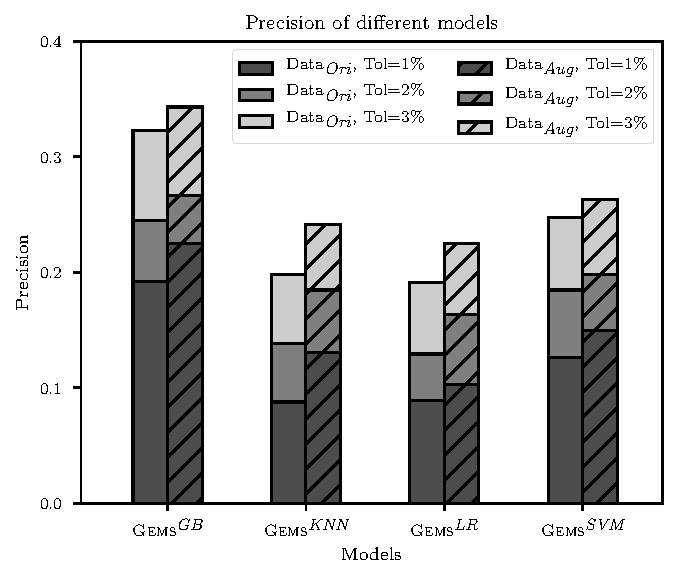
\includegraphics[width=0.49\linewidth]{Precision.pdf}}
\hfill
\subfigure[召回率]{\label{RQ3:recall}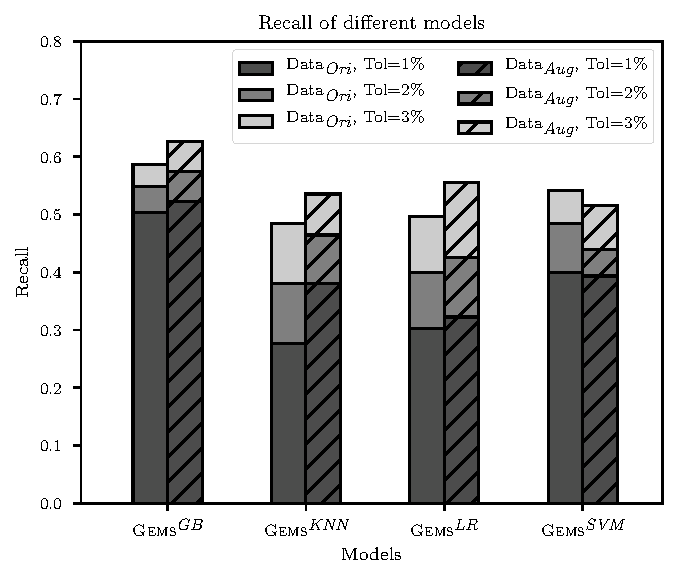
\includegraphics[width=0.49\linewidth]{Recall.pdf}}
\caption{训练数据集比较}
\label{dataset}
\end{figure}

图~\ref{dataset}为两组训练数据集在四个模型上的准确率和召回率。图~\ref{dataset}中斜条纹的柱形代表在扩
充数据集上的训练结果,没有斜条纹的柱形为在完全真实的数据上的训练结果;通过将容忍度设置为1\%、2\%和
3\%,得到在不同容忍度下模型的表现,在图~\ref{dataset}中依次用深灰色、灰色和浅灰色来表示。

通过观察图~\ref{dataset}中不同训练数据集的表现,可以得到以下结论:(1)在大部分情况下,使用扩充数据
集进行训练的模型表现优于使用原数据集训练得到的模型。只有在概率SVM模型中,原数据集的召回率略优于扩充
数据集,但该模型在扩充数据集上的准确率明显优于原数据集。这样的观察结果可能是因为扩充数据集的规模更
大,因此在大多数情况下具有更好的表现。(2)在KNN和LR中,扩充数据集对结果的改进要明显大于SVM和GBDT两个
模型。当使用原训练数据集时,LR和KNN的性能较差,可能是由于原数据集规模较小,由于数据不够多导致这两个
模型容易发生过拟合;而SVM由于最大间隔分类的原因,相比较LR和KNN不容易过拟合;类似的,GBDT为基于决策
树的融合模型,因此在小规模数据集上也能有较好的表现。

\subsection{梯度上升决策树和其它模型的比较}\label{RQ3}

\begin{figure}
\centering
\subfigure[准确率]{\label{RQ3:precision}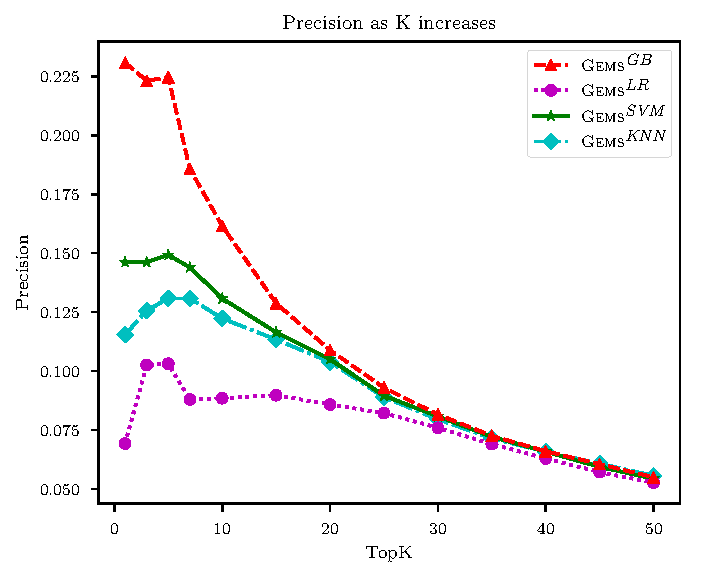
\includegraphics[width=0.49\linewidth]{topk_Precision.pdf}}
\hfill
\subfigure[召回率]{\label{RQ3:recall}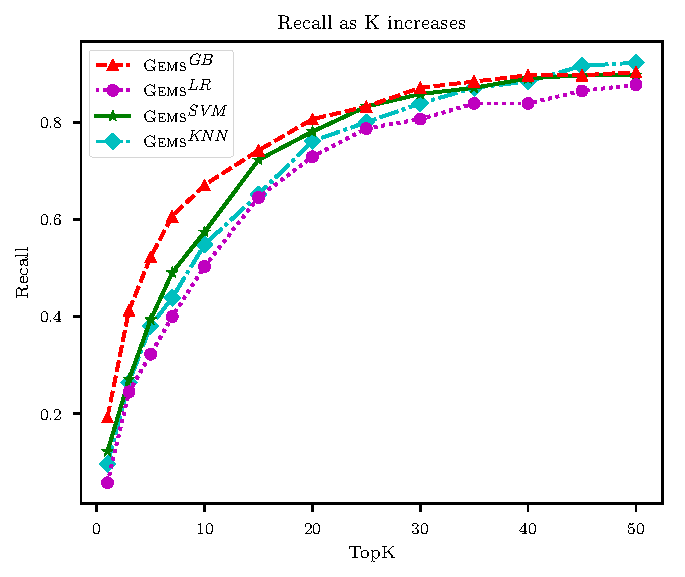
\includegraphics[width=0.49\linewidth]{topk_Recall.pdf}}
\caption{不同模型的准确率和召回率,横坐标表示推荐Top-$K$函数抽取重构机会}
\label{models1}
\end{figure}

为了评估梯度上升决策树模型在推荐函数抽取重构机会任务上的有效性,本节通过在不同特征组合上的表现来对以
下这四种模型进行对比。需要注意的是,虽然GEMS最终目的是为每个函数抽取重构机会预测其为正样本的概率,然
而两组训练数据集中都只包括正样本和负样本,因此对于部分无法直接预测类别概率的分类模型,还需要使用逻辑
斯特回归模型来做关于概率的训练,使分类器能够输出类别的概率。

具体来说,上述的四个模型中,只有梯度上升决策树和逻辑斯特回归模型可以直接预测给定样本为正例的概率,而最
近邻和支持向量机为分类模型,无法直接预测样本类别的概率。为了让分类器输出概率,在实验中使用逻辑斯特回
归,通过最大似然来拟合样本为正例的概率(Platt's scaling)。以概率SVM为例,传统的SVM针对给定测试样
本,根据训练好的参数计算出一个数值$y$,然后根据该数值是否大于0来预测该样本是否为正样本;概率SVM则以
第一阶段的输出$y$作为输入,样本的类别作为标签,通过逻辑斯特回归模型再训练,得到在输出为$y$时样本为正
例的概率。

图~\ref{models1}和图~\ref{models2}为当固定容忍度(1\%)和训练数据集(扩充数据集)时,GBDT、KNN、LR和
SVM四个模型的表现。其中红色代表GBDT,蓝色代表KNN,紫色代表LR,绿色代表SVM。横坐标为模型预测阶段,推
荐Top-$K$个函数抽取重构机会。从图~\ref{RQ3:recall}中可以看出,在大多数情况下GBDT的召回率略高于其它模
型;通过观察图~\ref{RQ3:precision}可以发现,GBDT的准确率相比较其它模型有很大优势,尤其推荐的函数抽取
重构机会较少时,GBDT的准确率明显高于其它模型。较高的准确率说明当推荐同样个数的函数抽取重构机会时,
GBDT模型推荐的模型更有可能被用户采纳,因此效率更高。

除此以外,通过观察图~\ref{models1}可以发现,当提高推荐的函数抽取重构机会数量时,召回率一直在上升,而
准确率则刚开始上升,达到峰值后迅速下降;最后当为每个函数推荐超过50个函数抽取重构机会时,召回率超过
92\%,而此时平均准确率降至0.05\%。图~\ref{models2}则更明显的反应了这一趋势,随着推荐的函数抽取重构机
会数量$K$的增加,F值先增长,大约当$K=5$时,四个模型的F值均达到峰值,然后随着$K$的增加,F值迅速降低。
基于以上观察,在实际使用GEMS的过程中,建议用户只看排名最高的5个函数抽取重构机会。

\begin{figure}
\centering
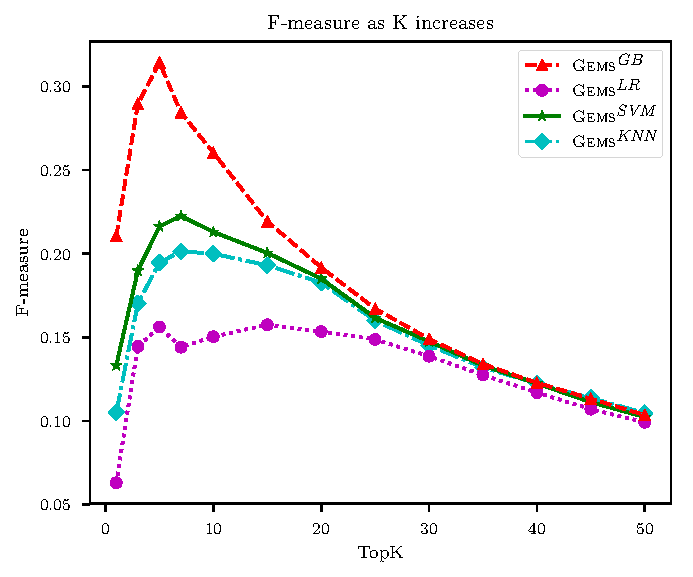
\includegraphics[width=0.49\linewidth]{topk_F-measure.pdf}
\caption{不同模型的F值,横坐标表示推荐Top-$K$函数抽取重构机会}
\label{models2}
\end{figure}

\subsection{针对长函数的实验结果}\label{RQ4}
由于函数抽取重构的目的之一是将长函数分解为短函数,因此本节针对实验数据集中的长函数进行对比实验。根据
之前的研究,长函数被定义为包括超过30行代码的函数~\cite{charalampidou2016identifying},表
~\ref{benchmark}中的实验对象一共包含15个长函数,涵盖了26个函数抽取重构机会。本节将GEMS与三种当前流行
的函数抽取重构推荐工具进行对比,评估GEMS处理长函数时的有效性。按照~\ref{canshu}中的参数设置方式,
GEMS、JExtract、SEMI和JDeodorant分别生成了1052、876、228和28个函数抽取重构机会。与之前的研究相同,为
每个函数最多保留排名最高的5个重构机会。表~\ref{long_methods}为在长函数上根据不同的容忍度统计得到的准
确率、召回率和F值。同样,黑体数值表示明显优于其它数值,而同等条件下的黑体数值之间相差在0.5\%以内,因
此被认为没有明显的区别。

通过观察表~\ref{long_methods}可以得到,在为长函数推荐函数抽取重构机会时,4个工具的结构均不如表
~\ref{accuracy}中的结果,说明了当面对长函数时,准确地推荐函数抽取重构机会存在一定的难度。不难发现,
当容忍度为1\%和2\%时,SEMI有最好的表现;当容忍度为2\%和3\%时,GEMS的表现最好。与表~\ref{accuracy}的
表现一样,JDeodorant由于其保守的函数抽取重构机会生成策略,准确率比JExtract高,同时JDeodorant的召回率
仍然是所有工具中最低的。当容忍度为1\%时,虽然GEMS的表现仍优于JExtract和JDeodorant,但其表现仍然不够
理想。然而,通过对实验数据进行分析,发现SEMI和GEMS对于长函数的表现差异,原因并不在于函数的规模,而在
于函数中存在的应该被抽取的函数片段较多。关于这个问题将在下一节中具体讨论。

\begin{table}[!t]
\zihaowu
  \renewcommand{\arraystretch}{1.3}
  % if using array.sty, it might be a good idea to tweak the value of
  % \extrarowheight as needed to properly center the text within the cells
  \caption{长函数准确性比较}
  \label{long_methods}
  \centering
  \begin{tabular}{cc|ccc}
  \toprule
   工具名称 &容忍度 &准确率 &召回率 &F值\\ 
  \midrule
  \multirow{4}{*}{GEMS$^{GB}$}&$1\%$ &13.3\% &31.9\% &18.8\% \\ 
  &$2\%$ &\bf{17.4\%} &\bf{41.5\%} &\bf{24.5\%} \\ 
  &$3\%$ &\bf{25.3\%} &\bf{46.2\%} &\bf{32.7\%} \\ 
  \hline
  \multirow{4}{*}{JExtract}&$1\%$ &6.6\% &16.1\% &9.4\% \\ 
  &$2\%$ &8.0\% &19.3\% &11.3\% \\ 
  &$3\%$ &8.0\% &19.3\% &11.3\% \\ 
  \hline
  \multirow{4}{*}{SEMI}&$1\%$ &\bf{16.4\%} &\bf{38.7\%} &\bf{23.0\%} \\ 
  &$2\%$ &\bf{17.9\%} &\bf{41.9\%} &\bf{25.0\%} \\ 
  &$3\%$ &19.1\% &45.1\% &26.9\% \\ 
  \hline
  \multirow{4}{*}{JDeodorant}&$1\%$ &12.0\% &9.6\% &10.7\% \\
  &$2\%$ &14.3\% &12.9\% &13.5\% \\ 
  &$3\%$ &16.0\% &12.9\% &14.2\% \\ 
  \bottomrule
  \end{tabular}
  \end{table}
  
\section{讨论}\label{discuss}
最后,本节就实验中发现的一些问题进行讨论。

\subsection{特征重要性}

尽管在实验中一共提取了48个特征进行训练,但这些特征的重要性并不完全相等。为了研究特征对实验结果的重要
性,使用过滤式特征选择(Relief特征选择算法)计算每个特征的相关统计量,然后使用不同的特征组合使用GBDT
进行训练。图~\ref{features}为使用不同数量的特征进行训练的实验结果,其中红色为召回率,绿色为准确率,
紫色表示F值。横坐标Top-$K$表示使用重要性最高的$K$个特征进行训练。

通过图~\ref{features}可以发现,当训练特征较少时,模型的表现较差。随着特征的数量逐渐增加,召回率、准
确率和F值随之增长。例如当特征的数量从5增加到35时,模型的准确率、召回率和F值分别提高了64.4\%、35.5\%
和55.8\%。然而,当继续增加特征的个数时,模型的表现逐渐降低。转折点大约出现在$K=35$处,因此有理由认为
并不是所有特征对模型训练都是有益的,48个特征中大约只有35个特征具有预测能力,而其它特征的加入只是引入
了噪音,可能导致模型效果降低。

  \begin{figure}
  \centering
  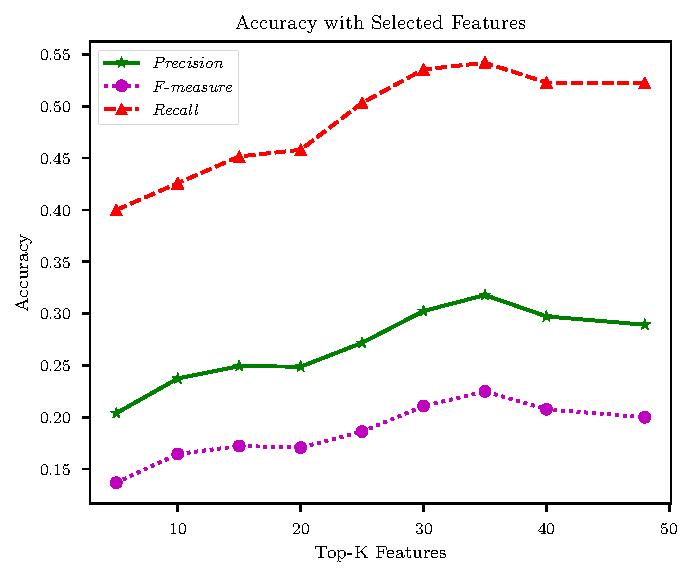
\includegraphics[width=0.49\linewidth]{fs.pdf}
    \caption{不同特征组合下的模型表现,横坐标表示使用Top-$K$个特征进行训练}
    \label{features}
  \end{figure}

表~\ref{important_features}中列出了按照特征重要性由高至低排名最高的20个特征。可以看到,排名较高的大
多为功能特征;特征``EXTRACTED\_LOCAL''的排名较高,意味着模型认为代码片段中是否含有本地变量的声明对决
定代码片段是否被抽取有较大影响;大多数与内聚度相关的特征(以``COHESION''结尾)在实验中被认为是比较重
要的。除此以外,表~\ref{important_features}中的排名说明了部分程序元素,如函数调用
(``INVOCATION'')、类型(``TYPE'')、包(``PACKAGE'')等比其它元素更重要,验证了本文研究动机中关于
软件质量度量由于考虑的程序元素较少,因此度量结果存在片面性的问题。

\begin{table}[!t]
\zihaowu
  \renewcommand{\arraystretch}{1.3}
  \caption{部分特征重要性排名}
  \label{important_features}
  \centering
  \begin{tabular}{p{1cm}c|p{1cm}c}
  \toprule 排名 &特征 &排名 &特征 \\ \midrule
  1& \textbf{INVOCATION\_COHESION}& 11& CON\_VAR\_ACC\\
  2& LOC\_EXTRACTED\_METHOD& 12& EXTRACTED\_LOCAL\\
  3& \textbf{TYPEDELE\_COHESION}& 13& CON\_LOC\\
  4& RATIO\_LOC& 14& EXTRACTED\_VAR\_AC\\
  5& CON\_PACKAGE& 15& \textbf{PACKAGE\_COHESION}\\
  6& EXTRACTED\_TYPED\_ELE& 16& CP\_PACKAGE\\
  7& CP\_VAR\_ACC& 17& CP\_PACKAGE2\\
  8& EXTRACTED\_PACKAGE& 18& \textbf{VARAC\_COHESION}\\
  9& \textbf{VARAC\_COHESION2}& 19& EXTRACTED\_IF\\
  10& CON\_INVOCATION& 20& EXTRACTED\_INVOCATION\\
  \bottomrule 
  \end{tabular}
  \end{table}
  
\subsection{多函数抽取重构机会}
通过观察针对长函数的实验数据,发现~\ref{RQ4}中所使用的长函数大多不止一个函数抽取操作(平均每个函数
1.9个),而GEMS的原理是预测候选函数抽取重构机会为正例的概率,并根据概率进行排序推荐。因此,不难理解,GEMS为相似的函数抽取重构机会分配相近的概率。同时,由于函数体内存在不止一个应该被抽取的代码片段,导致GEMS在为其中一个相关的函数抽取重构机会分配到高概率的同时,会为与其相似的其它重构机会分配较高的概率,因此导致其它不相似但应该被抽取的代码段的概率排名相对较低,最终导致了模型效率的下降。与GEMS相反,SEMI在推荐阶段将相似的函数抽取重构机会聚为一类,每次只从中选择排名最高的一个函数抽取重构机会进行推荐,从而取得了不错的表现结果。

针对上述问题,本文为使用者提供了两种策略:第一种,用户可以一步只进行一个函数抽取重构,在选定需要重构
的函数后,GEMS为用户推荐函数抽取重构机会列表,用户通过选择合适的重构机会让工具进行实施,在完成重构
后,若用户仍希望继续进行函数抽取,则再次选择该函数,进行下一轮的函数抽取重构推荐,直到使用者放弃重构
为止;(2)基于与SEMI类似的思路,可以将相似的函数抽取重构机会放到一组中,对于每组只推荐概率最高的函
数抽取重构机会给用户。具体来说,如果两个函数抽取重构机会$a$和$b$满足以下条件,则认为它们较为相似,可
以被放到一组:
\begin{eqnarray}
  \frac{\lvert{Start_a - Start_b}\rvert + \lvert{End_a - End_b}\rvert}{MAX(LoC_a, LoC_b)}\leq \it Threshold,
\end{eqnarray}
其中$Start$和$End$分别表示待抽取代码的起止行号;LOC为待抽取代码的行数,$Threshold$为设定的阈值。

\section{本章小结}
本章提出了基于梯度上升决策树的函数抽取重构机会推荐方法,并基于该方法开发了Eclipse插件GEMS。在训练阶
段,该方法首先每个训练样本提取两组特征,分别是结构特征和功能特征,融合了复杂度、内聚度和耦合度三个重
要的软件质量因素,以及多种与函数抽取重构相关的程序元素,并利用梯度上升决策树模型训练。在推荐阶段,针
对给定函数,首先使用基于代码块的方法生成所有合法的函数抽取重构机会,然后使用训练好的模型为每个函数抽
取重构机会分配一个概率,并根据概率由高至低推荐给用户。

通过在开源软件上进行实验,发现尽管GEMS生成了大量的函数抽取重构机会,但使用训练好的模型可以为好的函数
抽取重构机会分配较高的概率,使其排名较高,从而在实验中具有较好的表现。除此以外,受变异测试启发,本
文提出了使用函数内联重构来扩充训练数据集,并通过实验证明该训练集在大多数情况下能够取得比原训练数据集
更好的结果。值得注意的是,本文在构造扩充数据集时,谨慎地选择了具有良好设计模式的开源程序,并且只内联
被调用一次的函数作为待抽取片段,认为通过将该代码片段重新抽取出来能够提高程序的易读性、可维护性和可靠
性,与函数抽取的主要目的相一致。最后在不同模型上的实验结果证明了梯度上升决策树在推荐函数抽取重构机会
时的有效性,尤其当使用原数据集时,由于其融合模型的性质使得在小规模数据集上,该模型相比较其它三种模型
有较为明显的优势。通过分析特征重要性,本文发现了对函数抽取重构较为重要的因素,对了解函数抽取重构的意
图有一定程度的帮助。

本章具有以下贡献:

(1)提出了一个关于函数抽取重构的概率模型,通过学习从开源软件仓库中挖掘到的重构实例,模拟了软件维护
人员进行软件重构的过程,并考虑了函数抽取重构原因的多样性。

(2)提出了关于结构特征和功能特征的特征提取算法,融合了内聚度、耦合度、复杂度的软件质量概念,并考虑
了多种程序元素。

(2)设计并开发了一个基于Eclipse的插件GEMS,为给定Java函数生成函数抽取重构机会,并为每个合法的候选重
构机会分配一个概率,按照概率由高至低推荐给集成开发环境使用者。

(3)在开源程序上与主流函数抽取重构推荐工具的对比实验证明了GEMS的有效性,能够更准确地推荐函数抽取重
构机会,为软件维护人员提高维护效率。
% !TeX root = ../main.tex
% -*- coding: utf-8 -*-

\chapter{基于层次注意力的函数名推荐方法}
为了提高代码的易读性和易理解性,本章针对常见的软件重构操作--函数重命名重构进行研究。本章首先阐述了函
数名对软件系统的可维护性的重要性,然后介绍了关于函数重命名的相关研究现状。针对函数内在的层次结构,本
章提出了基于层次注意力模型的函数名推荐方法,该方法利用层次注意力,学习对函数中的源代码的分布式表示,
并利用该分布式表示预测函数名。在推荐阶段,通过集束搜索生成候选函数名序列,并按序推荐函数名,从而提高
软件系统的可维护性。

\section{引言}
随着当代软件系统的规模越来越大,软件维护所需的时间和人力成本也越来越高。一方面,随着需求的不断增加,
软件规模不断增大,导致软件系统的复杂度越来越高,可维护性降低。另一方面,软件维护通常建立在对软件系统
理解的基础上,软件维护人员需要花费大量的时间来理解和维护软件~\cite{Bansiya2002},如何快速理解并掌握
系统源代码成为维护人员经常需要面对的问题。

易读性是软件可维护性的重要组成方面,也是评估软件系统质量的关键因素
~\cite{buse2008metric}。研究者认为,在软件维护过程中,最耗费时间和精力成本的是阅
读代码的过程~\cite{rugaber2000use}。研究发现,大多数软件维护人员花费在阅读和理解
代码上的时间比真正花费在写代码上的时间更多~\cite{ko2006exploratory}。正因为此,
部分研究者提出在软件维护过程中,需要为阅读和理解代码预留出特定的时间,将代码易读
性作为代码检查的重要指标之一。

为了适应快速迭代的软件需求,当面对大规模软件系统时,软件维护人员通常不需要完全理
解和掌握代码的所有细节,才能对软件系统进行维护。在实践中较为常见的做法是通过阅读
函数的标题来理解函数的大致功能,通过多次跳转快速定位到与当前任务相关的代码位置
~\cite{starke2009searching}。只有当通过函数标题无法满足对函数理解的需求时,才会
仔细阅读具体的代码,获得更多的信息。

准确的函数名可以提高代码阅读的速度,从而提高软件维护的效率。在软件维护过程中,维护人员通过快速阅读代
码来理解程序的功能和行为。根据SRP原则~\cite{martin2003agile}(Single Responsibility
Principle),每个函数执行一个单独的功能,因此函数通常被认为是程序行为的最小单元
~\cite{host2009debugging}。准确的函数名能够总结函数的功能,因此通过阅读函数名,软件维护人员可以快
速理解函数的整体行为;相反,不准确的函数名通常导致理解和维护软件系统的难度提高
~\cite{arnaoudova2016linguistic},甚至在某些情况下可能导致代码缺陷~\cite{abebe2012can}。

函数重命名是完善性软件维护的重要手段。随着版本的不断更迭,新功能不断被添加,原本合适的函数名也可能变
得不再合适。此时,为了提高程序的易读性,防止由于函数名造成误导,需要进行函数重命名(Rename
Method),在不改变程序行为的前提下,通过更改函数名,提高软件系统的易读性和可维护性。Murphy等人
~\cite{Murphy-Hill:ICSE09}通过对13000位使用Eclipse的Java开发者进行调研,发现函数重命名是最常用的软件
重构类型之一。

尽管函数名对软件系统的易读性和可维护性具有较大的影响,但寻找具有总结能力且易读性强的函数名十分困难
~\cite{allamanis2015suggesting}。寻找好的函数名通常需要在理解函数的基础上,高度抽象整个函数的功能。
近年来,随着自然语言处理领域的不断发展,部分研究者将程序语言作为用来传递指令的一种特殊语言,将代码作
为一种特殊的文本进行学习。例如,Oda等人~\cite{oda2015learning}使用机器翻译技术将Python代码翻译成伪代
码,从而生成易读性更强的代码;Iyer等人~\cite{iyer2016summarizing}设计了一个将代码翻译成文本的神经注
意力模型,将长短期记忆神经网络(LSTM)和注意力机制应用于源代码和自然语言之间的翻译;
Movshovitz-Attias和Cohen~\cite{movshovitz2013natural}使用$n$-gram模型和主题模型从代码中生成评论。

尽管编程语言与自然语言之间存在一定的相似性,但其与自然语言在结构上有很大的区别。虽然自然语言的语法也
存在一定的结构性,但与程序语言相比,自然语言更加序列化和平铺直叙。与自然语言不同,程序语言中蕴含着丰
富的结构信息,直接将代码当做普通文本进行学习,得到的上下文信息不够准确,因此导致模型效果欠佳。

为了充分利用代码中的上下文信息,部分研究者~\cite{allamanis2015suggesting, haiduc2010supporting}通过
程序分析,从源代码中提取出一组与程序语义相关的特征,如Cyclomatic复杂度、变量类型和返回类型等,来表示
代码段。尽管这样的方法可以在一定程度上可以捕获到更精确的代码属性,但该方法依赖于特征工程的有效性,且
人为筛选特征的过程容易遗漏掉更多的语义信息。除此以外,Allamanis等人
~\cite{allamanis2016convolutional}提出使用卷积神经网络来学习代码的结构信息,通过加入注意力网络学习代
码对函数名预测的重要性。虽然卷积神经网络通常被认为适合学习结构特征,但卷积神经网络学到的是位置上的局
部特征,并非代码语义上的局部特征,因此导致其所捕获的上下文信息不够准确。

本文通过程序分析,将函数表示为由基本代码块组成的代码片段,利用代码的原始特征学习代码片段的分布式表示
(Distributed Representation)。与自然语言不同,代码具有明确的控制流结构,将程序行为拆分为多个由基本
块组成的子功能,每个基本块代表一个最小的功能单元;同时,一个代码块由多个词条组成,词条中含有丰富的语
义信息。基于这样的层次结构,本文通过使用层次注意力模型,分别学习基本代码块和词条(token)的重要性,
从而得到函数体的分布式表示并预测函数名。

本章主要有以下贡献:

(1)本章提出了基于层次注意力的函数名推荐模型,通过学习函数体的分布式表示,利用序列到序列模型为
给定函数推荐函数名。

(2)本章利用代码的层次结构,将代码表示为由基本块组成的代码片段,使用原始特征学习代码片段的分布式表
示,在代码搜索、克隆代码检测等领域有广泛的应用。

(3)在开源软件系统上的对比实验证明了基于层次注意力的函数名推荐模型的准确性,能够提高软件系统的易读
性和可维护性,从而提高软件维护效率。



\section{问题描述}\label{motivation3}
本文主要解决的是函数命名问题,即为代码片段预测具有语义的标识符。准确的函数名并不是简单描述代码的行
为,而是对代码段语义和功能的总结,因此好的函数名能够提高代码的易读性和易理解性,从而提高软件维护的效
率~\cite{takang1996effects}。

图~\ref{stop}中展示了来自Cassandra的示例代码片段以及本文方法的预测结果。Cassandra是一个开源的分布式
NoSQL数据库系统,其中函数的数量超过一万。当面对如此大规模的软件系统时,几乎一半的软件维护时间被用来
理解代码涵义上~\cite{corbi1989program}。为大型软件系统推荐具有语义的标识符作为函数名,能够减少维护人
员花费在阅读和理解代码上的时间。如图~\ref{stop}所示,本文使用基于层次注意力的模型,为示例代码片
段推荐了函数名候选列表,并为列表中的每个函数名分配了一个概率,按照概率由高至低推荐给用户。

虽然函数名重构对于提升软件易读性和可维护性有着重要的作用,但自动生成具有语义的函数名仍然存在以下困
难:

(1)不同于注释或者文档,函数名为由少数词项(Token)组成的标识符,因此函数名推荐需要在非常有限
的空间里总结函数的功能,同时忽略实现细节,这就要求模型具有较强的抽象能力和高层次的总结能力。

(2)不同于自然语言中的文本,程序代码具有高度结构性,通过明确的控制流信息将整体功能拆分成多个子功
能,因此学习并利用代码的结构信息,这就要求模型具有一定的结构学习能力。

(3)虽然函数名在整体上是对函数功能的总结和概括,但由于个人的命名习惯不同,导致很难推荐适用于所有用
户的函数名。

为了解决上述问题,本章提出了基于层次注意力的函数名推荐模型,利用代码的层次结构,将函数体拆分为多
个基本代码块,每个基本代码块由多个词项组成;利用注意力机制分别学习词项对基本块、基本块对函数体的
重要性,使模型能够识别对函数名预测有益的基本代码块和词项。最后,由于软件系统内部的代码风格通常较为一
致,因此通过使用相同软件系统中的函数命名实例作为训练数据集集,能够为用户推荐符合个性化命名习惯的函数
名。

除此以外,函数命名问题也是一种代码表示问题,即将代码表示为具有语义的矢量,使得具有相似语义的代码片段
能够有相近的表示。本章通过引入层次注意力,模拟代码段内部的层次结构,对给定代码片段进行分布式表
示,并学习基于分布式表示的函数名分布的条件概率,从而为给定代码片段预测函数名。除了预测标识符(变量
名、函数名和类名)以外,代码的分布式表示研究在克隆检测~\cite{white2016deep,allamanis2018learning}、
缺陷预测~\cite{murali2017finding}等领域也有广泛的应用。

\begin{figure}
\centering
\subfigure{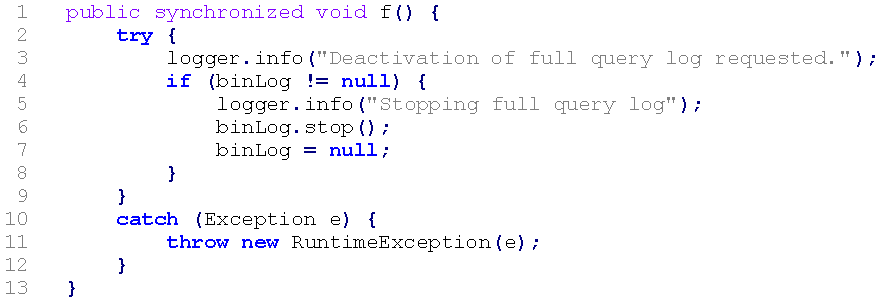
\includegraphics[width=0.82\linewidth]{stop.pdf}}
\hfill
\subfigure{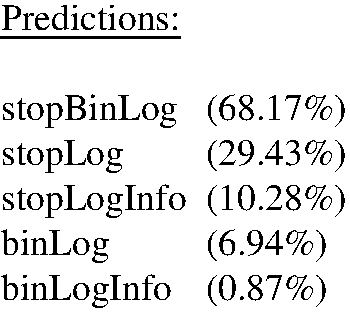
\includegraphics[width=0.17\linewidth]{prediction.pdf}}
\caption{示例代码段以及函数名预测}
\label{stop}
\end{figure}

\section{相关研究}
本节首先介绍了代码分布式表示模型,这些模型通过学习对代码的中间表示,将代码片段表示为难以直接解释的向
量。然后介绍了与代码属性预测模型,最后介绍了关于代码到自然语言的转换模型。

\subsection{代码表示模型}
在局部表示中,向量中的每个值通常有具体的明确的含义,例如在One-Hot表示模型中,当第$i$维数值为0时,表
示其对应的元素没有现在该样本中。与局部表示不同,分布式表示~\cite{hinton1984distributed}假设所表示的
元素可以在多维实数空间内进行编码,并且可以在该空间内评估两个表示之间的相关性。因此,分布式表示的结果
通常是一种矢量或矩阵,其元素的含义分布在多个维度上。由于具有较好的总结能力,分布式表示经常在自然语言
处理领域中被用来对自然语言中的元素进行编码。例如,Mikolov等人~\cite{mikolov2013efficient}通过学习自
然语言中单词的分布式表示,学到了单词之间的相关性。

由于在机器学习和自然语言处理上的成功运用,近年来,越来越多的研究者使用分布式表示模型表示代码,将代码
元素映射到矢量中。通过这样的方式,能够根据上下文学习代码的语义,具有相似上下文的代码通常具有相似的语
义。代码表示模型类似于自然语言处理中的文本表示模型,根据代码的表示代码表示模型可用来预测代码片段的属
性概率分布,如变量和函数名等。Mou等人~\cite{mou2016convolutional}使用自定义的卷积神经网络来学习代码
片段的分布式矢量表示,然他们混合了学生对各种课程问题的解决方案,通过分类来恢复这些解决方案到问题的映
射。Piech等人~\cite{piech2015learning}和Parisotto等人~\cite{parisotto2017neuro}学习了源代码输入/输出
对的分布式表示,并使用这些表示来评估和审查学生任务。除此以外,部分研究使用分布式表示来学习上下文信息
并生成代码。例如,Maddision等人~\cite{maddison2014structured}通过对上下文进行分布式表示,按序生成代
码。Ling等人~\cite{ling2016latent}和Allamanis等人~\cite{allamanis2015bimodal}将代码上下文分布式表示
与自然语言的分布式表示相结合来合成代码。Livshits等人~\cite{livshits2009merlin}通过分布式表示来解决信
息流问题。

\subsection{代码属性预测}
通过使用代码的抽象表示作为输入,得到关于代码属性在输入代码上的条件概率分布并进行预测代码的属性。
Allamanis等人~\cite{allamanis2014learning,allamanis2015suggesting,allamanis2016convolutional}发现变
量和函数名的分布式表示可以学到常见的语义属性,使用上下文信息学习变量和函数的分布式矢量表示,并使用这
种表示来预测变量名和函数名的概率分布。

Raychev等人~\cite{raychev2015predicting}将代码表示为变量依赖关系网络,将每个javaScript变量表示为一个
节点,并将其中的变量交互建模为条件随机场(CRF),最后通过联合预测代码片段中所有变量的类型和名称。受
统计机器翻译启发,Gu等人~\cite{gu2016deep}引入序列到序列的深度神经网络
~\cite{sutskever2014sequence},学习了自然语言查询的中间表示,并用来预测相关的API调用序列。Murali等人
~\cite{murali2017finding}利用主题模型的组合来学习一个循环神经网络,该神经网络为API调用序列建模。该模
型可来检测可能性极小的API调用序列,从而检测Android代码中实际存在的缺陷。除此以外,Allamanis等人
~\cite{allamanis2018learning}还通过学习将代码片段粘贴到现有的代码中,并调整所使用的变量来预测代码的
数据流图。Allamanis等人~\cite{allamanis2018learning}使用代码上下文中的各种元素来检测特定类型的缺陷,
如变量和操作符误用等。

\subsection{代码到自然语言的转换}
通过学习代码与自然语言文本的关系,可以自动生成代码文档,增加代码可读性。Oda等人
~\cite{oda2015learning}使用机器翻译技术将Python代码翻译成伪代码,从而生成易读性更高的代码;Iyer等人
~\cite{iyer2016summarizing}设计了一个将代码总结为文本的神经注意力模型。Movshovitz等人
~\cite{movshovitz2013natural}构建了一个推荐系统用来在给定源代码片段的情况下协助完成评论,该系统使用
类似主题的图模型来为上下文信息建模。

根据代码生成文本还可以用来自动生成注释。Sridhara等人~\cite{sridhara2010towards}提出了一种使用程序结
构信息为java函数生成摘要注释的方法,该方法的基本思想是从函数中选出重要的语句,然后将其翻译成自然语
言。该方法首先构建函数的数据流程图,然后分析该数据流来识别重要的语句。Wong等人
~\cite{wong2013autocomment}通过问答网站自动生成评论,从问题标题和回答文本中提取代码和描述的映射,并
使用代码克隆检测技术来查找与该映射相近的代码片段,查找出来的代码对通常是由开发人员从项目中复制的代
码,然后识别该代码片段的注释并重新应用于其他项目。然而,虽然这种方法可以应用于数百万个项目,但是其仅
对小部分代码片段有效,但无法为某个项目生成大量注释。

\section{研究方法}
本章提出了基于层次注意力的函数名推荐模型,该模型以编码-解码模型~\cite{Kyunghyun2014Learning}
(Encoder-Decoder)为基本框架,通过输出词项序列(Token Sequence)来为给定代码片段预测函数名。本节首
先简要阐述编码器-解码器的原理,然后介绍本章的模型架构,接下来依次介绍模型架构的各个组成部分,包括代
码片段的输入表示、编码器、解码器等;最后描述在预测阶段,针对给定的代码段,如何利用训练好的模型使用集
束搜索(Beam Search)生成具有概率的函数名列表。



\subsection{模型架构}


\subsubsection{编码-解码模型}
编码-解码模型为常见的一种模型框架,其核心思想是将输入$x$通过编码转化为一个向量$C$,再将向量$C$通过解
码转化为输出$y$。其中用来编码的模型为编码器(Encoder),用来解码的模型为解码器(Decoder)。编码器和
解器均可以为任意的模型;输入和输出也可以是任意的形式,如文字、图像等。当$x$和$y$均为序列时,这样的模
型也被称为序列到序列模型(Seq2Seq)。在实际应用中存在很多序列到序列的问题,例如翻译、问答系统等。

图~\ref{fig:seq2seq}为一个序列到序列模型的例子,其中编码器和解码器均使用循环神经网络(Recurrent Neural
Networks, 简称RNN)。给定输入序列$x=\{x_1,x_2,...,x_m\}$,该模型使用RNN将输入序列$x$编码为一个固定长
度的向量$C$,然后使用RNN将向量$c$解码为输出序列$y=\{y_1,y_2,...,y_n\}$,从而学习关于输出序列$y$在输
入序列$x$上的条件分布。在RNN中,第$t$个时刻的隐藏状态用$h_t$表示,该隐藏状态由前一个隐藏状态
$h_{t-1}$和第$t$个时刻的输入$x_t$共同决定:
\begin{eqnarray}
    h_t = f(h_{t-1},x_t),
\end{eqnarray}
因此,当输入完成时,当前隐藏状态$h_m$中包含了整个输入序列$x$的信息,通常将其作为输入序列$x$的编码
$C$。在解码阶段,同样使用RNN,以$C$作为输入,生成输出序列$y$,不同的是,生成$y_t$的概率还需要考虑已
经生成的输出$y_1,y_2...y_{t-1}$:
\begin{eqnarray}
    p(y_t|y_1,y_2,...,y_{t-1},C) = g(y_{t-1},H_t,C).
\end{eqnarray}
其中第$t$个时刻的隐藏状态$H_t$由前一个时刻的隐藏状态$H_{t-1}$和输出$y_{t-1}$以及输入的编码$C$共同决定:
\begin{eqnarray}
    H_t = f(H_{t-1},y_{t-1},C).
\end{eqnarray}
通过这样的方式,可以在输入序列的长度$m$和输出序列的长度$n$不相等的情况下,构建一个关于输出序列$y$在
输入序列$x$上的条件分布的生成模型$p(y_1,y_2,...,y_n|x_1,x_2,...,x_m)$,然后通过最大似然的方式拟合数
据集。

\begin{figure} [!t]
	\centering
	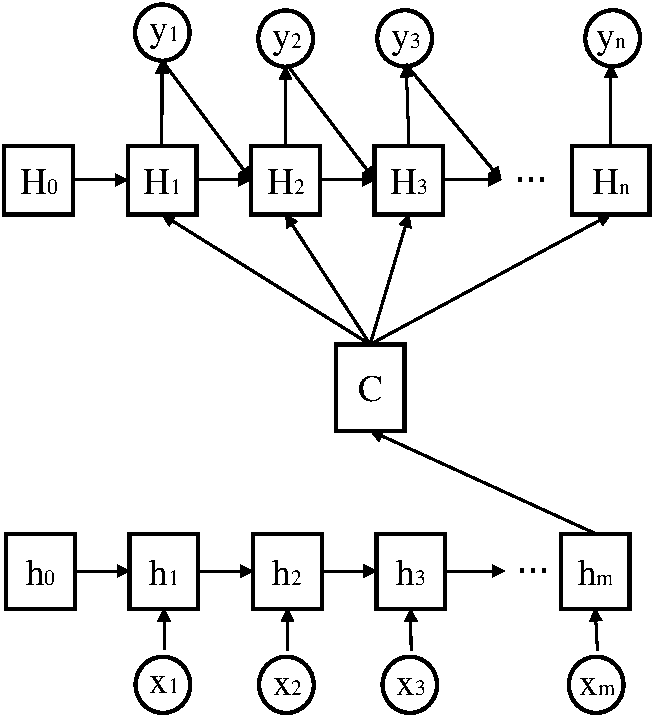
\includegraphics[width=0.45\textwidth]{seq2seq.pdf}
	\caption{RNN编码-解码模型}
	\label{fig:seq2seq}
\end{figure}

本章提出的基于层次注意力的函数名推荐模型,与上述模型有相似的架构,均为序列到序列的编码-解码模型。两
者的区别是,本文使用层次注意力作为编码器将代码段表示为固定长度的向量,然后使用GRU序列模型作为解码
器,通过学习函数名关于代码段的条件概率分布,输出构成函数名的词项序列(Token Sequence)。

\subsubsection{函数名推荐模型架构}
本章模型的架构如图~\ref{fig:arch}所示。可以看出,该模型为编码-解码模型
~\cite{Kyunghyun2014Learning}。为了提高模型的抽象和总结能力,本文使用程序分析将函数功能拆分为多个由
基本代码块组成的子功能,不同基本代码块对预测函数名的重要性不同;同时,一个代码块由多个词项组成,不同
的词项的重要性也不同。为了模拟这样的层次结构,在编码阶段引入层次注意力模型
~\cite{yang2016hierarchical}分别学习基本代码块和词条(token)对预测函数名的重要性,通过编码-解码模型
学习函数名在代码片段上的条件分布。

\begin{figure} [!t]
	\centering
	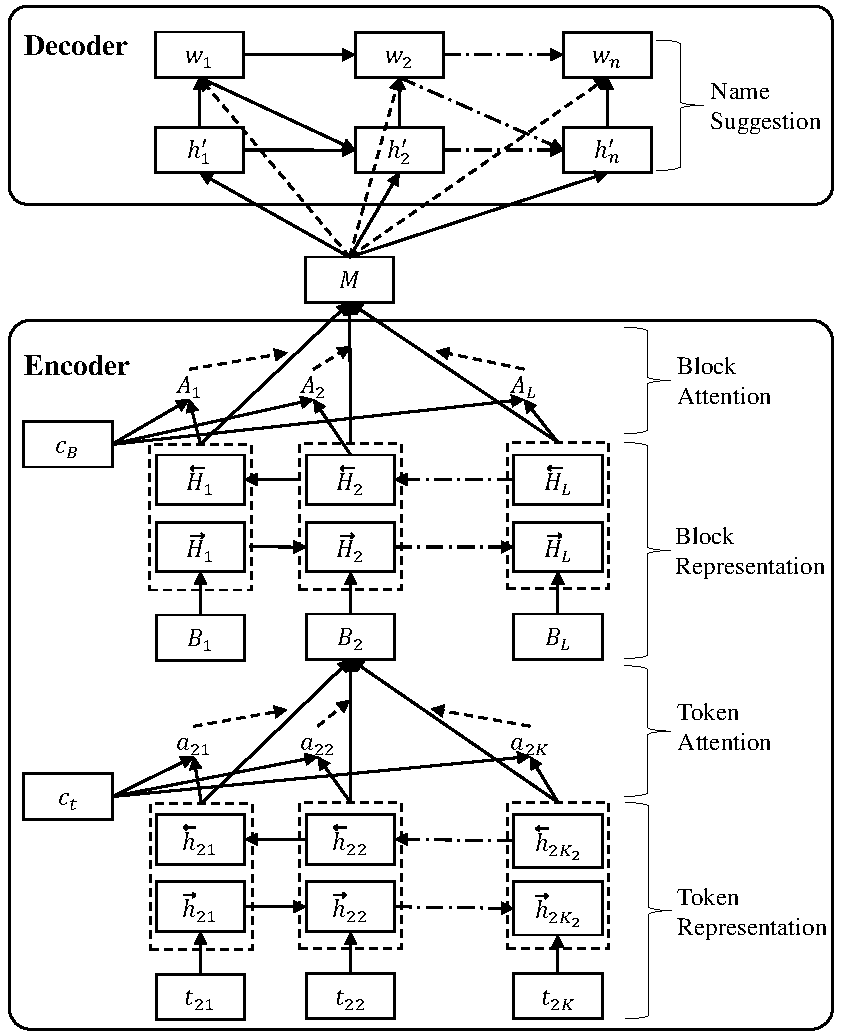
\includegraphics[width=0.65\textwidth]{architecture.pdf}
	\caption{基于层次注意力的函数名推荐模型架构}
	\label{fig:arch}
\end{figure}

如图~\ref{fig:arch}所示,编码器对代码片段的表示分为两个阶段:在第一阶段,给定输入的词项序列,学习基
本代码块的表示;在第二阶段,以基本代码块序列列作为输入,学习整个代码片段(函数体)的表示。 在解码阶
段,以代码片段的表示作为输入,使用门控循环单元~\cite{Kyunghyun2014Learning}模型学习组成函数名的词项
序列在代码片段上的条件分布。同样,在计算当前隐藏状态$h_t'$时考虑上一个时刻的输出$w_{t-1}$,使模型能
快速收敛。

基于层次注意力的函数名推荐模型,其输入是由基本代码块序列构成的代码片段,输出是由词项序列构成的函
数名。给定函数$m$,将其表示为由基本代码块组成的序列$m=(B_1,B_2, \dots, B_L)$,每个基本块由词项序列表
示,例如$B_2 = (t_{21}, \dots, t_{2K_2})$,其中$K_2$为基本代码块$B_2$中所包含的词项的个数。模型的输
出为词项序列$(w_1, \dots, w_n)$,表示预测的函数名。需要注意的是,输入和输出序列的长度可以不一致,事
实上,与代码的长度相比,函数名的长度通常非常短,因此为给定代码片段预测函数名的困难较大。

编码器首先根据输入的基本代码块序列,通过层次注意力将函数体表示为一个固定长度的向量$M$:
\begin{equation}
M = f({B_1, \dots, B_L}) \,.
\label{eq:encoder}
\end{equation}
然后解码器依次预测组成函数名的词项,根据上一个时刻的词项和解码器的输出向量$M$,预测当前时刻的词项:
\begin{equation}
P(w_j|\{w_1, \dots, w_{j-1}\}, M) = g(\{w_1, \dots, w_{j}\}, M) \,,
\label{eq:decoder}
\end{equation}
其中$g$的输出为一个概率,表示根据代码片段的表示向量$M$和上一个时刻的输出词项$w_{j-1}$,预测当前词项
为$w_j$的概率,本文使用softmax激活函数使函数$g$的输出为一个概率值。

将解码器和编码器联合起来,能够学习关于函数名的词项序列$w$在由词项组成的代码段$t$上的条件分布
$p(y|t)$,最后通过最大条件对数似然来优化该联合模型:
\begin{equation}
\max \limits_{\bm\theta} \frac{1}{N}\sum_{n=1}^{N} \log p_{\bm\theta}(\bm w_n | 
\bm t_n) \,,
\label{eq:loss}
\end{equation}
其中$N$表示训练样本的个数,$\bm\theta$为模型中的参数,通过使用随机梯度下降来优化模型的参数。

\subsection{输入代码段表示}
\label{represent}
为了提高模型的抽象和总结能力,本文将函数体拆分为多个基本代码块,每个代码块作为执行函数子功能的最小单
元,通过注意力机制学习不同基本代码块对函数名预测的重要性。

借鉴于程序指令中基本块的定义,本文将基本代码块定义如下:
\begin{Definition}
    基本代码块。基本代码块为顺序执行的代码语句,每个基本代码块有且只有一个入口和出口。
\end{Definition}

为了对函数体进行划分,首先根据函数的控制流信息将函数中的代码片段表示为如图
~\ref{block-example}所示的代码结构树。根据基本代码块的定义,每个基本代码块有且只有一
个入口,且基本块中的语句是顺序执行的,因此对基本代码块的划分主要依赖于对代码基本
块入口的寻找。给定函数$m$以及其代码结构树$Tree(m)$,通过遍历其代码结构树来寻找函
数体中的入口语句集合$E(m)$。算法~\ref{alg:block}描述了获取入口语句集合的遍历过
程。具体来说,首先对于函数$m$,其中第一条语句一定是入口语句,因此将其加入入口语
句集合中;通过宽度优先算法遍历函代码结构树$Tree(m)$,从左往右依次判断节点是否为
叶子节点;若该节点不是叶子节点,则访问下一个节点;若该节点是叶子节点,且其左兄弟
不是叶子节点,则将该节点对应的语句加入入口语句集合中;否则继续访问下一个节点。

在找到所有的入口语句后,对函数中代码片段的划分过程为:按照代码的顺序,从函数的第
一个入口语句开始,直到遇到下一个入口语句或是函数结束,为一个基本代码块。以图
~\ref{block-example}中的代码和代码结构树为例,按照算法~\ref{alg:block}可以得到入
口语句为$(S_2,S_4,S_6,S_9,S_{12},S_{16})$,因此根据上述过程可将示例函数划分为6个
基本代码块,每个基本代码块为顺序执行的代码语句。

\begin{algorithm}[H]
\caption{入口语句搜索算法}\label{alg:block}
\KwIn{函数$m$;}\\
\KwOut{入口语句集合$E(m)$;}\\
获取函数$m$的代码结构树$Tree(m)$;\\
将函数入口语句加入集合$E(m)$;\\
初始化所有节点的状态为未访问;\\
初始化队列$queue=\emptyset$;\\
将根节点压入队列queue;\\
\While {$queue \neq \emptyset$} {
    从队列中移除并返回头顶节点作为当前节点;\\
    \If {当前节点为叶节点} {
        \If {当前节点的左兄弟不是叶子节点且不在集合$E(m)$中} {
            将当前节点的对应语句加入集合$E(m)$;\\
        }
    }
    \Else{
        将当前节点的所有未被访问的子节点加入队列$queue$;\\
    }
    标记当前节点的状态为已访问;\\
}
\textbf{return} 入口语句集合$E(m)$。\\
\end{algorithm}

在将函数体进行划分后,得到基本代码块序列$m=\{B_1, \dots, B_L\}$,其中每个代码基
本块为一个词项序列$B_i=\{t_{i1},t_{i2},\dots,t_{iK_i}\}$。需要注意的是,由于函数体
中标识符的存在,因此对程序语言的分词除了根据非英文字符以外,本文对标识根据两种命
名惯例进行分词,分别是下划线命名法(如set\_params)和驼峰命名法(如setParams或
SetParams)。通过这样的方式,得函数体的层次结构表示作为模型的输入。


\subsection{基于层次注意力的编码器}
在编码阶段,本文采用层次注意力模型将给的那个代码片段表示为固定长度的向量。接
下来自底向上详细阐述本章模型中的编码器。

\subsubsection{门控循环单元}
基于层次注意力的函数名推荐模型,在编码器和解码器中都使用了门控循环单元
~\cite{Kyunghyun2014Learning}作为基础模型。门控循环单元(Gated Recurrent Unit,简称GRU)通过门控机制
处理远距离依赖,其效果与同样使用门控机制处理远距离依赖的长短期记忆模型~\cite{Hochreiter1997Long}
(Long Short-Term Memory,简称LSTM)相差不多,但由于GRU的参数较少,因此收敛速度较快,所需要的样本较
少~\cite{Chung2014Empirical}。

GRU模型的门控机制包括两个门计算,分别重置门和更新门。前者用于控制当前时刻的输入如何与上一个时刻的信
息相结合,后者用于控制上一个时刻的信息被保留到当前时刻的程度,通过这样的方式,GRU模型能够控制以前的
信息被保留和遗忘的程度,从而在一定程度上解决了RNN的梯度消失的问题。

\begin{figure} [!t]
	\centering
	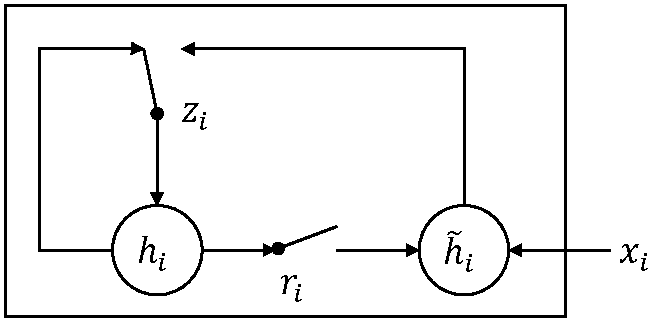
\includegraphics[width=0.35\textwidth]{gru.pdf}
	\caption{门控循环单元示意图}
	\label{fig:gru}
\end{figure}

图~\ref{fig:gru}为GRU模型的门控示意图,其中$z_s$和$r_s$分别表示第$s$个时刻的更新门和重置门。更新门$z_s$控制了过去信息和输入信息中需要被继续传递的部分,通过以下公式进行计算:
\begin{equation}
    z_s = \sigma (W_z x_s + U_z h_{s-1} + b_z) \,,
    \label{eq:gru_update}
\end{equation}
$x_s$为第$s$个时刻的输入向量,$h_{s-1}$为上一个时刻的隐藏状态,$W_z$和$U_z$为权重矩阵,$b_z$为偏差。
公式~\eqref{eq:gru_update}通过对$x_s$和$h_{s-1}$分别进行线性变换,再将这两部分信息相加并使用激活函数
得到更新门$z_s$,更新门的存在使模型能够有选择性地保留过去记忆和当前输入中的信息。

图~\ref{fig:gru}中的$r_s$为重置门,重置门根据过去记忆和当前输入,决定了过去记忆被忽略的程度。重置门
的计算公式与更新门类似,但参数不同:
\begin{equation}
    r_s = \sigma (W_r x_s + U_r h_{s-1} + b_r) \,,
    \label{eq:gru_ret}
\end{equation}
其中$W_r$和$U_r$为权重参数,$b_r$为偏差,$x_s$为当前的输入,$h_{s-1}$为上一个时刻的隐藏状态。

接下来阐述更新门$z_s$和重置门$r_s$是如何帮助模型有选择性地将过去的记忆与当前的输入相结合,并继续传递
的。首先根据重置门对过去记忆的存储选择,可以得到新的记忆内容:
\begin{equation}
    \tilde{h}_s = \tanh (W_h x_s + r_s \odot (U_h h_{s-1}) + b_h) \,,
    \label{eq:gru_cand}
\end{equation}
其中新的记忆内容由两部分组成,第一部分为输入信息$x_s$,第二部分为重置门$r_s$控制的过去记忆,重置门通
过Hadamard乘积控制过去记忆$h_{t-1}$被保留的程度,通过将这两部分信息相加,得到当前的新记忆内容
$\tilde{h}_s$。

最后通过更新门控制对当前记忆和过去记忆的传递程度,计算得到当前时刻的隐藏状态:
\begin{equation}
	h_s = (1-z_s) \odot h_{s-1} + z_s \odot \tilde{h}_s \,,
    \label{eq:gru_h}
\end{equation}
其中$z_s$为更新门,控制了当前记忆$\tilde{h}_s$和过去记忆$h_{s-1}$中需要传递的信息。更新门和重置门让
模型能够有选择的控制过去记忆的保留和传递,从而使得模型在能够捕捉长期依赖的前提下减少梯度消失。


\subsubsection{词项表示}
给定函数体$m=\{B_1,B_2,\dots,B_L\}$,其中的每个基本代码块都由词项表示。本章模型的主要任务是为给定函
数体预测函数名,因此首先要将函数体中的词项用向量表示。具体来说,首先针对给定训练数据集中的词项构建一
个字典,过滤掉频率过低的词项。对于函数体中的每个基本代码块$B_i=\{t_{i1},t_{i2},\dots,t_{iK_i}\}$,词
嵌入矩阵$W_e$将词项$t_{ij}$转化为向量$x_{ij}=W_e t_{ij}$,然后使用双向GRU模型学习基本代码块
的表示,对于每个输入词项$t_{ij}$,从两个方向获取其上下文信息。对于每个基本代码块$B_i$,前向
GRU从$t_{i1}$到$t_{iK_i}$读取词项,后向GRU从$t_{iK_i}$到$t_{i1}$读去词项:

\begin{align}
	x_{ij} &= W_e t_{ij} \quad\text{(Embedding)} \,, \\
	\overrightarrow{h}_{ij} &= \overrightarrow{GRU}(x_{ij}) 
	\quad\text{(Forward GRU)} \,, \\
       \overleftarrow{h}_{ij} &= \overleftarrow{GRU}(x_{ij}) 
       \quad\text{(Backward GRU)} \,, \\
       h_{ij} &= [\overrightarrow{h}_{ij}, \overleftarrow{h}_{ij}] 
       \quad\text{(Concatenation)} \,,
\label{eq:token_encoder}
\end{align}
其中$j\in [1, K_i] \cap N^+$。在从两个方向计算出词项的隐藏状态后,双向
GRU模型将这两个隐藏状态连接起来作为该词项的表示。需要注意的是,本文中
的词嵌入矩阵$W_e$并没有使用预训练好的词嵌入矩阵,而是通过高斯分布随机初始化
词嵌入矩阵$W_e$,该矩阵在训练过程中随模型的其它参数一起优化。根据双向GRU模型中的隐藏状
态,每个词项得到一个向量表示,该表示考虑了两个方向的上下文信息。

\subsubsection{词项注意力}
在函数$m$中,每个基本代码块由一个词项序列表示
$B_i=\{t_{i1},t_{i2},\dots,t_{iK_i}\}$,然而并不是每个词项对于基本代码块的表示都
具有同等的重要性。例如,在代码``int sum = len1 + len2;''中,词项``int''对于代码
功能的重要性大概率低于词项``sum''。因此,为了学习不同词项对基本代码块的重要性,
引入了注意力机制为每个词项分配一个权重:

\begin{align}
    u_{ij} &= c_t^\top \tanh(W_t h_{ij} + b_t) \,, \\
    a_{ij} &= \frac{\exp{u_{ij}}}{\sum_{j^\prime=1}^{K_i} \exp{u_{ij^\prime}}} 
    \,, \\
    B_{i} &= \sum_{j=1}^{K_i} a_{ij}h_{ij} \,,
\label{eq:token_attn}
\end{align}
其中$j\in [1, K_i] \cap N^+$,$c_t$为词项级别的上下文向量表示,在训练
中与其它参数一起学习,$W_t$表示词项的权重参数,$b_t$为偏差,并使用Softmax函数将权重规则化。最
后,每个基本代码块通过组成该基本块的词项的权重和来表示。

\subsubsection{基本代码块表示}
在表示基本代码块时,同样考虑了基本代码块的上下文信息,因此使用类似的双向GRU模型
来获取其上下文信息。给定函数$m$,将其通过基本代码块序列表示,即$M = (B_1, \dots,
B_L)$,每个基本代码块$B_i$的隐藏状态为:
\begin{align}
    \overrightarrow{H}_i &= \overrightarrow{GRU}(B_{i}) 
\quad\text{(前向GRU)} \,, \\
    \overleftarrow{H}_i &= \overleftarrow{GRU}(B_i) 
\quad\text{(后向GRU)} \,, \\
    H_i &= [\overrightarrow{H}_i, \overleftarrow{H}_i] 
\quad\text{(连接)} \,,
\label{eq:block_encoder}
\end{align}
其中$i\in [1, L] \cap N^+$。双向GRU模型通过从两个方向来表示基本代码块$B_i$的上下
文信息,通过这种方式,同样可以得到每个基本代码块的隐藏状态表示。

\subsubsection{基本代码块注意力}
本文将函数体表示为由基本代码块组成的序列,虽然本文假设每个基本代码块完成函数的一
个子功能,但不同基本块完成的子功能不同,其对函数整体功能的影响也不同。为了让模型
能够学到不同基本代码块对函数名预测的重要性,在使用基本代码块表示函数体时,再次引
入了注意力机制,为每个基本代码块分配不同的权重。用$c_B$表示每个基本代码块对预测
函数名的重要性,可以得到:

\begin{align}
v_i &= c_B^\top \tanh(W_B H_i + b_B) \,, \\
A_i &= \frac{\exp{v_i}}{\sum_{i^\prime=1}^{L} \exp{v_{i^\prime}}} 
\,, \\
M &= \sum_{i=1}^{L} A_i H_i \,,
\label{eq:block_attn}
\end{align}
其中$i\in [1, L] \cap N^+$,$c_B$在随机初始化后,通过优化模型得到;$W_B$是基本代码块的权重参数,$b_B$
为其对应的偏差。最后函数体的表示向量$M$通过基本代码块的权重和得到。通过这样的方式,表示向量$M$通过层
次的方式对整个函数的信息进行编码,在编码时考虑了不同词项对基本代码块表示的重要性可能不同,也考虑了不
同基本代码块对函数表示的重要性可能不同,并在接下来的解码器中作为输入预测组成函数名的词项序列。

\subsection{基于门控循环单元模型的解码器}
为了预测函数名,在解码阶段使用另一个GRU模型将通过编码器得到的函数表示$M$转化为词项序列
$\{y_1,y_2,...,y_K\}$。如公式~\eqref{eq:decoder}所示,在第$k$个时刻,输出为$y_k$的概率与函数在解码器
中的编码$M$和前面已经生成的输出$y_1,y_2,...,y_{k-1}$相关。需要注意的是,由于理论上函数名与代码片段不
在同一个空间,因此函数名中的词项$y$与输入代码段中的词项$t$具有不同的表示,即词项$y_k = W_w w_k$,其
中$W_w$为另一个词嵌入矩阵。

为了表示在解码器中,第$k$个时刻的输入为上一个时刻的输出$y_{k-1}$和函数表示$M$,将公式
~\eqref{eq:gru_update}--\eqref{eq:gru_h}中关于GRU模型的计算过程稍作修改,增加了函数表示$M$作为输入:
\begin{align}
z_k &= \sigma(W_z y_k + U_z h^\prime_{k-1} + \underline{V_z M} + b_z) \,, \\
r_k &= \sigma(W_r y_k + U_r h^\prime_{k-1} + \underline{V_r M} + b_r) \,.\\
\tilde{h}^\prime &= \tanh(W_h y_k + r_k \odot (U_h h^\prime_{k-1}) + 
\underline{V_h M} + 
b_h) \,, \\
h^\prime_k &= (1-z_k)\odot h^\prime_{k-1} + z_k \odot \tilde h^\prime_k \,, 
\end{align}
其中增加函数表示$M$作为输入的部分用下划线标记出来,$V_{*}$为增加的输入向量$M$的权重参数。同样使用更
新门和重置门控制对过去记忆$h^\prime_{k-1}$的保留和遗忘。在得到第$k$个时刻的隐藏状态$h^\prime_k$后,
使用Softmax激活函数来预测第$k$个时刻输出词项为$y_k$的概率:
\begin{align}
p(y_k&|\{y_{k-1}, \dots, y_1\}, M) \notag\\
&= \text{softmax}(W_o(y_{k-1} + W_{h^\prime}h^\prime_k + W_M M) + b_o) \,,
\label{softmax}
\end{align}
其中$W_o$、$W_{h^\prime}$和$W_M$为Softmax层的参数,$b_o$为偏差。公式~\eqref{softmax}在计算第$k$个时刻
输出为$y_k$的概率时,将$y_{k-1}$作为和函数的表示向量$M$作为输入,通过这种强制教导(Teacher
Force~\cite{Williams1989learning})的方式提高模型训练的效率。

\subsection{集束搜索函数名推荐}
在测试阶段,给定输入函数体$m$,通过在每个时刻选择概率最大的词项作为输出,直到输出结束符号为止,能够
得到一个词项序列$\{y_1,y_2,\dots,y_m\}$。将输出的词项序列按照命名惯例组合起来,则得到为给定函数体$m$
预测的函数名。然而,这种生成方式只能预测一个函数名。为了尽可能接近最优解,本文通过在预测阶段使用集束
搜索(Beam Search),为给定函数体生成一个函数名列表,从而扩大用户的选择范围。

集束搜索为序列到序列模型中常用的启发式搜索方式~\cite{Graves2012Sequence,sutskever2014sequence},这种
搜索方式在本质上基于贪心思想,但由于其扩大了搜索范围,因此能够得到更多的解。假设集束宽度为2,在第一
个时刻选择概率最大的两个词项$y_{11}$和$y_{12}$,将$y_{11}$和$y_{12}$分别当作第一个时刻的词项$y_1$,
通过公式~\eqref{softmax}得到在给定$y_1$的情况下词项$y_2$的条件概率$p(y_2|y_1,m)$,根据公式
~\eqref{beam}可以得到给定输入函数体$m$时,输出词项序列为$y_1,y_2$的概率。选择概率最大的两个词项序
列,重复上述的过程,直到遇到结束符号位置。通过这样的方式,可以为给定函数体$m$生成具有概率的函数名候
选集。
\begin{align}
p(y_2,y_1|m) = p(y_2|y_1,m)p(y_1|m) \,,
\label{beam}
\end{align}

\section{实验设计}
本节评估了基于层次注意力的函数名推荐模型的有效性,通过在10个开源软件系统上进行实
验,对比评估了基于层次注意力的模型与其它三种模型推荐函数名的准确性,验证了本章方
法的有效性。

\subsection{实验对象与数据处理}
本章的实验对象为10个来自GitHub的开源软件系统。表~\ref{benchmark3}为实验对象的统
计数据,可以看出,本章的实验对象为GitHub上收藏和使用较多的开源软件系统,且规模较
大。由于大规模软件系统的维护成本和维护难度较高,因此提高大型软件系统的易读性和维
护效率具有重要的意义。


为了根据不同软件系统的代码习惯推荐个性化的函数名,同时与之前的研究保持一致,在实
验中针对每个软件系统训单独训练一个函数名推荐模型。具体来说,对于表
~\ref{benchmark3}中的每个软件系统,首先提取其中所有的函数,并过滤掉其中的抽象函
数、构造函数和重写函数。过滤掉抽象函数是因为模型的输入为构成函数体的代码
片段,而抽象函数没有代码片段,无法正常预测;过滤掉构造函数是因为构造函数的函数名
与类名相一致,因此对函数名的推荐类似于推荐类名称,与本文模型的主要目的不同;过滤
掉重写函数是因为重写函数由于重复的原因,在模型中很容易预测。
通过这样的方式,针对每个软件系统能够获得一个函数样本集,将样本集随机打乱,并将其
中80\%的样本作为训练数据,10\%的样本作为验证数据,剩下的10\%作为测试数据来评估模
型在该软件系统上的有效性。

\begin{table}[!t]
\zihaowu
\renewcommand{\arraystretch}{1.4}
% if using array.sty, it might be a good idea to tweak the value of
% \extrarowheight as needed to properly center the text within the cells
\caption{实验对象统计数据}
\label{benchmark3}
\centering
\begin{tabular}{l@{\quad}l@{\quad}l@{\quad}l@{\quad}l}
\toprule 
软件名称 &规模(M) &函数数量 &收藏数量 &使用数量\\ 
\midrule
Apache Cassandra &11.1 &10,466 &4,502 &2,061\\ 
Elasticsearch &19.8 &15,409 &32,393 &11,104\\ 
Gradle &14.1 &16,050 &7,096 &2,227\\ 
Hadoop-common &37.5 &33,237 &121 &141\\ 
Hibernate-orm &21.6 &34,307 &3,275 &2,250\\ 
Intellij-community &5.84 &6,972 &6,182 &2,362\\ 
Liferay-portal &47.9 &52,539 &1,258 &2,114\\ 
Presto &11.0 &10,672 &7,755 &2,616\\ 
Spring-framework &29.3 &33,157 &22,182 &14,313\\ 
Wildfly &14.2 &9,566 &2,012 &1,805\\ 
\bottomrule
\end{tabular}
\end{table}

对于数据集中的每个函数,将其作为一个样本,函数体是为样本的输入代码段,函数为样本
的标签。对于除本章方法以外的三个模型,通过分词的方式将函数体和函数名进行表示为词
项序列,对于代码中与函数名相同的标识符,使用词项``SELF''进行代替,其余标识符则根
据两种命名惯例进行分词,分别是下划线式(my\_case)与驼峰式(myCase或MyCase),从
而得到样本的输入序列和输出序列。在评估本章模型时,需要将输入序列表示为具有层次结
构的词项和基本代码块序列。最后,利用训练集对模型进行训练,并通过验证集调整超参,
例如基本代码块中词项序列的最大长度、隐藏单元的个数等,并在测试集上评估方
法的有效性。为了使实验具有可重复性,已将本次实验的数据集发布。

\subsection{对比实验}
为了评估本章方法的有效性,将其与词频-逆文件频率算法、循环神经网络和卷积神经网络三个模型进行对比实
验。其中,词频-逆文件频率算法(Term Frequency–Inverse Document Frequency,简称tf-idf算法)为信息检索
领域常用的一种统计方法,其核心思想通过对比词项在文档中出现的频率与词项在数据库中出现的频率来判断词项
的重要性。在本章实验中,由于在构建词项字典时已经统计了每个词项在所有函数体中出现的频率,因此使用
tf-idf算法为给定函数体推荐函数名,只需要统计输入词项序列中每个词项在输入中出现的频率即可。由于函数名
推荐的本质是对函数功能的翻译和总结,因此本章还使用了在机器翻译领域有较好表现的双向RNN-attention模型
~\cite{bahdanau2015neural},该模型在双向RNN的基础上加入了注意力机制,被认为可以学习输入序列与输出序
列之间的权重关系。除此以外,本章还将基于层次注意力的函数名推荐模型与基于卷积神经网络和注意力机制的函
数名推荐模型~\cite{allamanis2016convolutional}(以下简称为CNN-attention模型)进行对比,该方法通过卷
积神经网络学习代码结构的局部特征。与该方法不同的是,本文将程序分析与注意力机制相结合,将函数拆分为多
个基本代码块,并学习每个基本代码块对函数名的重要性。最后,在训练阶段,使用推荐的参数对RNN-attention
和CNN-attention模型进行训练。在训练基于层次注意力的模型时,使用Adam梯度下降算法
~\cite{kingma2014adam}作为优化器,并使用了dropout~\cite{srivastava2014dropout}来防止模型过拟合。

\subsection{评估方法}
本章从函数名和词项两个角度评估函数名推荐模型的准确性。其中,函数名的匹配被定义为从开始符号起到第一个
结束符号为止,预测的词项序列与代表函数名的词项序列完全一致。而词项级别的评估方法则以词项为单位,不考
虑词项的顺序,只考虑词项的准确率、召回率和F值。具体来说,准确率表示预测的词项中正确预测的词项所占的
百分比;召回率表示函数名的词项序列中被成功预测到的词项所占的百分比;如公式~\ref{f1}所示,F值为这两者
的加权调和平均。需要注意的是,虽然通过集束搜索能够得到多个解,在实验中为每种模型只选择概率最高的解作
为该模型的最终预测结果。

\section{实验结果与分析}
本节从函数名与词项两个角度比较了基于层次注意力的函数名推荐方法与其它三种较为流行
的模型在函数名推荐任务上的表现。

\subsection{函数名推荐方法比较}
表~\ref{accuracy3}为函数名的匹配率比较,即对测试样本进行预测时,预测结果与样本中
的函数名完全一致的函数占总数的百分比。第一列为实验中所使用的模型,从上至下依次代
表tf-idf算法、基于循环神经网络与注意力机制的模型~\cite{bahdanau2015neural}(表中
简写为RNN)、基于卷积神经网络与注意力机制的函数名推荐模型
~\cite{allamanis2016convolutional}(简写为CNN)以及本章提出的基于层次注意力的模
型(简写为HIER)。表~\ref{accuracy3}中使用黑体表示被标记的数值具有明显优势,而同
一列中的两个黑体数值之间则没有明显的区别(+/-0.5\%以内)。

\begin{table}[!t]
\scriptsize
\renewcommand{\arraystretch}{1.3}
\caption{匹配率比较}
\label{accuracy3}
\centering
\begin{tabular}{ccccccccccc}
\toprule
方法 &Cassandra &Elasticsearch &Gradle &Hadoop &Hibernate &Intellij &Liferay &Presto &Spring &Wildfly\\ 
\midrule
TF-IDF&30.4\%&13.7\% &15.6\% &21.9\%&47.3\% &11.4\% &53.2\% &25.6\% &\bf{23.1\%} &22.9\%\\ 
RNN&23.9\% &8.9\% &12.0\%  &13.4\% &51.1\% &5.7\% &48.1\% &18.3\% &15.4\% &19.2\%\\ 
CNN& 27.6\% &17.5\% &19.3\% & 22.5\% &58.9\% &\bf{13.4\%} &59.2\% &23.8\% &21.9\% &\bf{23.6\%}\\ 
HIER&\bf{31.7\%} &\bf{18.3\%} &\bf{20.6\%} &\bf{24.1\%} &\bf{62.0\%} &12.8\% &\bf{63.7\%} &\bf{26.1\%} &\bf{23.5\%} &\bf{23.7\%}\\
\bottomrule
\end{tabular}
\end{table}

从表~\ref{accuracy3}可以看到,除了Hibernate和Liferay,四个模型在其它所有数据集上
的匹配率均不高(在5.7\%\textasciitilde31.7\%之间),表明了函数名预测任务存在一定
的难度。不难发现,在其中9个数据集上基于层次注意力的模型的匹配率高于或等于其它三
种模型,证明了该模型在函数名预测任务上的有效性。CNN模型取得了仅次于本文模型的匹
配率,而tf-idf和RNN模型的匹配率则相对较低。对于这样的实验结果,一个可能的原因是
CNN模型~\cite{allamanis2016convolutional}与本章模型都是针对函数名预测任务而提出
的,并在模型中通过不同的方式考虑了代码的结构信息;而tf-idf与RNN模型
~\cite{bahdanau2015neural}是针对文档提出的,因此在模型中没有考虑代码的结构信息。
除此以外,通过观察成功预测的函数名,发现大多数匹配的函数名所包含的词项较少,说明
对长函数名预测的难度更大。

\begin{table}  
\scriptsize
\caption{词项级准确性比较}  
\label{token-accuracy}
\centering  
\subtable[词项级准确率]{ 
\begin{tabular}{ccccccccccc}
\toprule
方法 &Cassandra &Elasticsearch &Gradle &Hadoop &Hibernate &Intellij &Liferay &Presto &Spring &Wildfly\\ 
\midrule
TF-IDF&41.7\% &31.4\% &34.9\% &40.4\% &47.3\% &33.1\% &64.9\% &50.3\% &38.1\% &48.8\%\\ 
RNN   &38.2\% &29.9\% &30.6\% &31.1\% &47.2\% &23.8\% &58.4\% &41.6\% &33.3\% &36.5\%\\ 
CNN   &50.4\% &34.7\% &\bf{40.9\%} &\bf{41.3\%} &62.4\% &\bf{35.1\%} &66.7\% &\bf{51.6\%} &37.6\% &48.9\%\\ 
HIER  &\bf{51.6\%} &\bf{35.4\%} &\bf{41.4\%} &\bf{41.5\%} &\bf{64.8\%} &34.2\% &\bf{69.3\%} &\bf{52.1\%} &\bf{42.0\%} &\bf{49.6\%}\\
\bottomrule
\end{tabular} 
\label{tab1}  
}  \\
 
\subtable[词项级召回率]{          
\begin{tabular}{ccccccccccc}
\toprule
方法 &Cassandra &Elasticsearch &Gradle &Hadoop &Hibernate &Intellij &Liferay &Presto &Spring &Wildfly\\ 
\midrule
TF-IDF&41.9\% &28.5\% &31.4\% &35.3\% &55.2\% &28.4\% &63.7\% &44.0\% &39.7\% &45.2\%\\ 
RNN   &35.1\% &21.8\% &25.3\% &26.7\% &54.5\% &21.2\% &55.1\% &37.9\% &30.6\% &29.7\%\\ 
CNN   &48.1\% &\bf{33.5\%} &35.3\% &\bf{39.2\%} &59.7\% &\bf{32.0\%} &\bf{67.8\%} &\bf{47.1\%} &39.5\% &45.1\%\\ 
HIER  &\bf{50.4\%} &32.9\% &\bf{36.9\%} &\bf{38.9\%} &\bf{63.8\%} &30.1\% &\bf{68.2\%} &\bf{47.4\%} &\bf{41.3\%} &\bf{47.1\%}\\
\bottomrule
\end{tabular}
\label{tab2}  
}  


\subtable[词项级F值]{          
\begin{tabular}{ccccccccccc}
\toprule
方法 &Cassandra &Elasticsearch &Gradle &Hadoop &Hibernate &Intellij &Liferay &Presto &Spring &Wildfly\\ 
\midrule
TF-IDF&41.8\% &29.9\% &33.1\% &37.9\% &54.6\% &30.6\% &63.9\% &46.9\% &38.4\% &46.9\%\\ 
RNN   &36.6\% &25.2\% &27.7\% &28.7\% &50.6\% &22.4\% &56.7\% &39.7\% &31.9\% &32.8\%\\
CNN   &49.2\% &\bf{34.1\%} &37.9\% &\bf{40.2\%} &61.0\% &\bf{33.9\%} &67.2\% &\bf{49.2\%} &38.5\% &46.9\%\\
HIER  &\bf{51.0\%} &\bf{34.1\%} &\bf{39.0\%} &\bf{40.1\%} &\bf{64.3\%} &32.0\% &\bf{68.7\%} &\bf{49.6\%} &\bf{41.6\%} &\bf{48.5\%}\\
\bottomrule
\end{tabular}
\label{tab3}  
}
\end{table} 

由于完全匹配两个序列的难度较高,为了比较预测结果与函数名的相似性,在实验中统计了
正确预测词项的情况来评估预测结果是否与函数名具有相似的语义。表
~\ref{token-accuracy}列出了四种模型在数据集上的词项级准确率、召回率和F值。可以看
到,词项级的准确率和召回率比匹配率明显更高,说明在某些情况下,虽然模型没有正
确预测给定代码片段的函数名,但仍然学到了部分的语义。同样,在表
~\ref{token-accuracy}中用黑体标记了每列中最大的一个或多个数值。可以发现,39个最
大数值中的26个数值为层次注意力模型的预测结果,13个为CNN模型的预测结果,证明了本
文方法能够在一定程度上预测出能够表达函数功能的关键词项;同时也反映了在编码阶段通
过层次注意力网络对代码片段的表示能够获得有效的代码语义信息。除此以外,tf-idf相比
较RNN模型取得了更好的结果,一个可能的解释是函数名中存在很大部分的词项来自于其对
应的函数体,且在该函数体中出现的频率高于在其他函数中出现的频率。

\subsection{操作符对模型的影响}
程序语言通常包括关键字、标识符、操作符以及其它特殊符号组成,为了评估程序语言中的
操作符对代码片段表示的影响,本文设计了一组对比试验,通过改变所有数据集的预处理方
式,评估模型是否能够学到操作符等特殊符号中所包含的语义。例如,是否能根据操作符学
习到与函数功能相关的语义。

具体来说,本节通过在数据预处理阶段采取不同的处理方式,得到两组不同的数据集,其中
一组训练数据、验证数据和测试数据中均不存在操作符,另一个为原来的数据集。表
~\ref{operator}为在四个模型上使用上述两组数据集得到的在所有软件上的平均匹配率、
词项准确率、词项召回率和词项F值。其中在包含操作符的数据集上进行实验的结果用
$w/i$表示,在不包含操作符的数据集上实验的结果用$w/o$表示。根据表~\ref{operator}
中的结果,可以发现从整体上看在两组数据集上的结果并没有很大的区别,说明当前这四种
模型主要通过关键词和标识符学习代码片段与函数明的语义关系。

\begin{table}[!t]
\zihaowu
\renewcommand{\arraystretch}{1.4}
\caption{不同与处理方式的比较}
\label{operator}
\centering
\begin{tabular}{cccccccc}
\toprule
 方法 &预处理方式 &匹配率 &词项准确率 &词项召回率 &F值\\ 
\midrule
\multirow{2}{*}{TF-IDF}&w/i&29.9\%&42.3\% &43.6\% &41.8\% \\ 
&w/o&29.3\% &41.9\% &44.1\% &41.4\% \\ 
\multirow{2}{*}{RNN}&w/i&19.3\% &37.1\% &36.0\%  &35.4\% \\ 
&w/o&18.7\% &37.3\% &36.5\% &35.8\% \\
\multirow{2}{*}{CNN}&w/i& 27.7\% &60.4\% &41.3\% &44.9\% \\ 
&w/o&26.3\% &60.2\% &37.1\% &43.6\% \\
\multirow{2}{*}{HIER}&w/i&30.1\% &57.1\% &44.7\% &46.2\% \\
&w/o&29.8\% &57.3\% &42.2\% &45.8\% \\
\bottomrule
\end{tabular}
\end{table}

\section{讨论}




\begin{table}[!t]
\scriptsize
\renewcommand{\arraystretch}{1.3}
% if using array.sty, it might be a good idea to tweak the value of
% \extrarowheight as needed to properly center the text within the cells
\caption{基于层次注意力的函数命名样例}
\label{samples}
\centering
\begin{tabular}{l||l} 
\toprule
函数 \& 预测结果 &函数 \& 预测结果 \\
\midrule
\tabincell{l}{
      %\includegraphics[scale=0.7]{1.pdf}
      {\color{blue}{public}} ByteBuffer \textbf{getIndexedValue}() \{\\
 \quad {\color{blue}{return}} clustering.get(indexedColumn.position());\\
    \}}
&\tabincell{l}{
      %\includegraphics[scale=0.7]{1.pdf}
      {\color{blue}{public boolean}} \textbf{isDataPresent}() \{\\
 \quad {\color{blue}{return}} !responses.isEmpty();\\
    \}}\\ 
 \tabincell{l}{\underline{Predictions}: \\getPositionValue (38.67\%), 
    getPosition (22.64\%), \\getIndex (15.21\%), get (3.87\%), column (1.36\%).}&
 \tabincell{l}{\underline{Predictions}: \\isEmpty (32.14\%),
    empty (17.41\%), responses (5.46\%), \\getResponses (3.61\%).}\\
 \hline
 \tabincell{l}{
      %\includegraphics[scale=0.7]{1.pdf}
      {\color{blue}{public long}} \textbf{getRepairedAt}() \{\\
 \quad {\color{blue}{return}} sstableMetadata.repairedAt;\\
    \}}
&\tabincell{l}{
      %\includegraphics[scale=0.7]{1.pdf}
      {\color{blue}{int}} \textbf{getHeartBeatVersion}() \{\\
 \quad {\color{blue}{return}} version;\\
    \}}\\ 
\tabincell{l}{\underline{Predictions}: \\getMinRepairedAt (24.91\%), 
    getRepairedAt (20.07\%), \\metadata (9.54\%), getMetadata (5.48\%), sstable (1.48\%).}&
\tabincell{l}{\underline{Predictions}: \\getVersion (42.47\%),
    version (18.07\%), get (2.87\%).}\\
\hline
 \tabincell{l}{
      %\includegraphics[scale=0.7]{1.pdf}
      {\color{blue}{public boolean}} \textbf{isClean}() \{\\
 \quad {\color{blue}{return}} partitions.isEmpty();\\
    \}}
&\tabincell{l}{
      %\includegraphics[scale=0.7]{1.pdf}
      {\color{blue}{private void}} \textbf{notifyCreateKeyspace}(...) \{\\
 \quad changeListeners.forEach(l -> l.onCreateKeyspace());\\
    \}}\\ 
\tabincell{l}{\underline{Predictions}: \\isEmpty (29.91\%), partition (15.32\%), \\empty (9.62\%), getPartition (3.15\%), clean (1.23\%).}&
\tabincell{l}{\underline{Predictions}: \\notifyNewKeyspace (38.25\%), createKeyspace (16.21\%), \\notifyKeyspace (12.54\%), keyspace (9.32\%).}\\
 \hline
\tabincell{l}{
      %\includegraphics[scale=0.7]{1.pdf}
      {\color{blue}{public static}} BoostingQueryBuilder \textbf{boostingQuery}() \{\\
 \quad {\color{blue}{return new}} BoostingQueryBuilder(positiveQuery);\\
    \}}
&\tabincell{l}{
      %\includegraphics[scale=0.7]{1.pdf}
      {\color{blue}{public}} BigArrays \textbf{getBigArrays}() \{\\
 \quad {\color{blue}{return}} bigArrays;\\
    \}}\\ 
\tabincell{l}{\underline{Predictions}: \\addQuery (36.13\%), 
    buildQuery (24.73\%), \\boostingQuery (14.22\%), query (3.41\%), build (1.62\%).}&
\tabincell{l}{\underline{Predictions}: \\getBigArrays (51.23\%),
    bigArrays (24.75\%), \\getArray (14.02\%), array (1.25\%).}\\   
 \hline
\tabincell{l}{
      %\includegraphics[scale=0.7]{1.pdf}
      {\color{blue}{public}} ByteSizeValue \textbf{getBufferSize}() \{\\
 \quad {\color{blue}{return}} bufferSize;\\
    \}}
&\tabincell{l}{
      %\includegraphics[scale=0.7]{1.pdf}
      {\color{blue}{void}} \textbf{setBackPressureEnabled}(...) \{\\
 \quad conf.back\_pressure\_enabled = backPressureEnabled;\\
    \}}\\ 
\tabincell{l}{\underline{Predictions}: \\getBufferSize (26.83\%), 
    bufferSize (15.58\%), \\getSize (9.81\%), sizeOf (1.78\%).}&
\tabincell{l}{\underline{Predictions}: \\setBackPressureEnabled (34.63\%), set (15.41\%) \\
 BackPressureEnabled (10.34\%), enable (5.67\%).}\\      
 \hline
\tabincell{l}{
      %\includegraphics[scale=0.7]{1.pdf}
      {\color{blue}{public static}} RecoveryStats \textbf{readRecoveryStats}(...) \{\\
 \quad RecoveryStats stats = {\color{blue}{new}} RecoveryStats(); \\
 \quad stats.readFrom(in);\\
 \quad {\color{blue}{return}} stats;\\
    \}}
&\tabincell{l}{
      %\includegraphics[scale=0.7]{1.pdf}
      {\color{blue}{protected}} BulkByScrollResponse \textbf{buildResponse}() \{\\
 \quad {\color{blue}{return new}} BulkByScrollResponse(took, task.getStatus(),\\
  \quad \quad \quad \quad \quad \quad indexingFailures, searchFailures, timedOut);\\
    \}}\\ 
\tabincell{l}{\underline{Predictions}: \\readFromStats (22.63\%), 
    getStats (12.21\%), \\createRecoveryStats (4.36\%), RecoveryStats (1.07\%).}&
\tabincell{l}{\underline{Predictions}: \\newResponse (16.72\%),
    createResponse (10.63\%), \\BulkByScrollResponse (9.23\%), index (0.46\%).}\\      
 \hline
\tabincell{l}{
      %\includegraphics[scale=0.7]{1.pdf}
      {\color{blue}{public static}} UUID \textbf{maxTimeUUID}({\color{blue}{long}} timestamp) \{\\
 \quad {\color{blue}{long}} uuidTstamp = fromUnixTimestamp(timestamp) - 1;\\
 \quad {\color{blue}{return new}} UUID(createTime(uuidTstamp), \\
 \quad \quad \quad \quad \quad \quad \quad MAX\_CLOCK\_SEQ\_AND\_NODE);\\
    \}}
&\tabincell{l}{
      %\includegraphics[scale=0.7]{1.pdf}
      {\color{blue}{public}} ColumnMetadata \textbf{getDroppedColumn}(...) \{\\
 \quad DroppedColumn dropped = droppedColumns.get(name); \\
 \quad {\color{blue}{return}} dropped == {\color{blue}{null}} ? {\color{blue}{null}} : dropped.column;\\
    \}}\\ 
\tabincell{l}{\underline{Predictions}: \\getTimeUUID (32.93\%), 
    getUUID (10.13\%), \\createTime (5.26\%), maxUUID (4.39\%), timestamp (0.36\%).}&
\tabincell{l}{\underline{Predictions}: \\getDroppedColumn (26.02\%), compareDropped (13.31\%), \\getName (8.24\%),
    dropped (17.27\%), column (10.89\%).}\\        

\bottomrule
\end{tabular}
\end{table}

为了直观基于层次注意力的函数名推荐模型是如何为给定代码片段推荐函数的,表~\ref{samples}列举了一些来自
Cassandra和Elasticsearch的函数。以每个函数的函数体作为输入代码片段,并使用集束搜索得到最多5个词项序
列作为推荐的函数名列表,并按照概率大小排序。需要注意的是,由于本文模型的输入并不包括函数的参数,因此
为了简洁,列举的函数中省略了函数本身的参数。

从表~\ref{samples}中可以看出,对于一些简单的函数,例如对于$getBufferSize()$和
$getBigArrays()$函数,模型能够很容易地预测出准确的函数名。通过分析实验中的预测结
果,发现模型能够较为准确地识别简单的$get$和$set$类型的函数,然后通过$(get|set)+
variable$的模式对函数名进行预测。这种方法在很多情况下能够正确预测函数名,但有时
也会与真实的函数名不一致。例如表~\ref{samples}中的$getHeartBeatVersion()$函数,
模型预测结果为$getVersion()$。

通过观察表~\ref{samples}中的$isDataPresent()$和$isClean()$函数,可以发现,这两个
函数的代码段有相似之处,即都使用$isEmpty()$函数判断变量是否为空。虽然这两个函数
中的变量名不同,但由于模型在预测时为它们的共同词项$is$和$empty$分配了较大的权
重,使得这两个函数具有相似的表示,从而得到相同的预测结果。

最后本文通过实验发现,由于函数命名存在一定的主观性,而目前的评估方法很难准确评估
函数名推荐的准确性。如表~\ref{samples}中的函数$buildResponse()$,本文模型的预测
结果中概率最大的候选函数名为$newResponse$。按照现有的评估方式,该函数的匹配率为
0,词项准确率和召回率均为$50\%$,但从直观上看,这两个函数名具有类似的含义,也从
侧面证明了本文模型能够在一定程度上学到代码片段的语义。

\section{本章小结}
为了提高程序的易读性和可维护性,在软件维护过程中维护人员需要频繁的通过函数重命名
的重构方式,改善现有的函数名,使其能够精准地总结现有函数的功能,从而减少代码阅读
时间。目前已经有越来越多的研究者关注于程序代码的自动理解与表示。为了更好地学习函
数体中的代码,本章利用程序的控制流信息,将函数体拆分为由多个基本代码块组成的序
列,通过层次注意力模型分别学习基本代码块与整体函数的表示,并通过学习函数名在函数
表示上的条件分布来为给定代码片段预测函数名。

通过在10个大规模开源软件上的对比试验,证明了本文方法在函数名推荐任务上的有效性。
除此以外,本章设计了关于不同数据预处理方式的对比试验,通过实验评估了代码片段中的
操作符对模型的影响,发现现阶段的4个模型均不能学习到操作符中所蕴涵的语义知识。最
后,通过对实验数据进行分析,发现当前模型能够较为准确地预测出简单函数的函数名,且
在一定程度上能够学到代码段之间的语义关系。


% !TeX root = ../main.tex
% -*- coding: utf-8 -*-
\chapter{总结与展望}
本章对本文的主要研究内容、创新点以及所解决的问题进行了总结,并通过对未来研究方向
的展望,提出了关于研究工作的进一步的想法和建议。

\section{研究内容总结}
软件维护是贯穿软件生命周期的重要软件活动,占据了整个软件生命周期中的大部分时间。
随着用户需求的不断添加,软件系统的规模和复杂度也不断提高,导致软件维护的难度越来
越大。与此同时,软件系统通常需要快速迭代才能适应当代社会日新月异的改变与需求,为
软件维护的效率和性能带来了重大的挑战。

本文的研究内容主要针对软件维护中最重要的两个软件维护类型--纠错性软件维护和完善性
软件维护。纠错性软件维护通过尽可能早地发现软件系统中存在的缺陷,使得软件能够正确
地运行,是完善性软件维护的基础;同时,完善性软件维护通过改进软件设计、提高软件系
统的易读性、可靠性和可维护性,能够提高纠错性软件维护的效率,并减少新缺陷的引入。

本文的研究方法为通过数据驱动的方法,挖掘数据中的潜在规律作为软件维护问题的解决方
案。虽然目前很难制定出完整而严密的规则来完全自动化进行软件维护,但软件维护的过程
是存在规律的,并不是随机的、无章可循的。数据挖掘为这种存在潜在规律但很却难通过规
则完美解决的难题提供了一种新的解决方案。与此同时,随着科技的发展,开源社区和版本
控制工具的成熟也为数据挖掘提供了大量可用的数据。从数据的角度来理解软件维护的过
程,将软件维护问题转化为数据挖掘问题,能够在提高软件维护效率和性能的同时,减少软
件维护的成本。

为了提高纠错性和完善性软件维护的效率和性能,本文通过数据挖掘的方法完成了以下研究
工作:

第一,为了提高纠错性软件维护的效率,本文研究了基于覆盖分析的多缺陷定位问题。由于
开发过程中很难发现所有潜在的缺陷,软件系统中存留的缺陷可能导致软件行为失效。为了
提高纠错性软件维护的效率,研究者提出了很多缺陷定位方法来尽可能早地发现导致软件行
为失效的原因。其中,基于覆盖分析的缺陷定位方法由于只需要统计测试用例执行时的覆盖
信息,通过特定的公式估算代码的可疑度来定位缺陷,而不需要对源代码进行建模和分析,
因此计算成本较低,在面对大规模软件系统时适用性较强。然而,现有的基于覆盖分析的缺
陷定位方法大多假设被失效用例执行越多、成功用例执行越少的代码越可疑。这种假设虽然
在单缺陷程序中可能性较大,但面对多缺陷程序时,由于造成程序失效的原因不止一个,因
此即使是缺陷相关代码也可以不被失效用例所覆盖。由于很难区分由不同缺陷导致的失效用
例,导致现有的基于覆盖分析的缺陷定位方法在面对多缺陷程序时的定位效率下降。为了提
高多缺陷程序的定位效率,本文受特征选择启发,提出了缺陷相关统计量,为每个失效用例
寻找距离最近的失效用例,作为最有可能与其由相同缺陷触发的失效用例。通过计算特征对
样本类别的重要性,找到覆盖后容易导致测试用例执行失效的特征,将其作为可能的缺陷相
关代码,从而进行缺陷定位。


第二,为了提高完善性软件维护的效率,本文研究了关于函数抽取重构机会的识别和推荐。
随着对软件系统的不断修改,软件系统越来越偏离原来的设计,导致软件系统的质量越来越
低。为了提高软件质量,需要及时对软件系统进行重构。针对最常用的重构类型之一,函数
抽取软件重构,目前已经有很多研究者提出了自动识别和推荐重构机会的方法。大多数函数
抽取重构机会推荐方法通过软件质量度量来评价候选重构机会。虽然提高软件质量是软件重
构的主要原因,但与纠错性软件维护不同,完善性维护很难有统一的、明确的标准来量化维
护的效果。除此以外,考虑到函数抽取软件重构的原因具有多样性,根据软件质量度量进行
函数抽取机会推荐的结果往往只能得到满足某种特定软件质量度量的重构机会,因此效果通
常不甚理想。为了解决这个问题,通过挖掘开源软件仓库中的函数抽取重构实例,并在特征
提取算法中融合了复杂度、内聚度和耦合度三个与函数抽取重构相关的重要软件质量概念以
及多种程序元素,本文构建了关于函数抽取重构机会的概率模型,学习如何进行函数抽取重
构。除此以外,通过对特征重要性进行分析,探索了函数抽取重构的原因,从而进一步理解
了软件维护人员进行函数重构的意图。

第三,为了提高软件系统的易读性和可维护性,本文研究了函数重命名的问题。在软件维护
过程中,最耗费时间和精力成本的是阅读代码的过程。准确的函数名可以提高代码阅读的速
度,从而提高软件维护的效率;不准确的函数名通常导致理解和维护软件系统的难度提高,
甚至在某些情况下可能导致代码缺陷。尽管函数名对软件系统的易读性和可维护性具有较大
的影响,但寻找具有总结能力且易读性强的函数名十分困难。随着自然语言处理技术的发
展,很多研究者将程序语言作为一种特殊语言,使用自然语言处理技术将代码当作文本来学
习。尽管编程语言与自然语言之间存在一定的相似性,程序语言中蕴含着丰富的结构信息,
直接将代码当做普通文本进行学习,得到的上下文信息不够准确,容易导致模型效果欠佳。
为了利用代码结构中所蕴含的信息,本文通过控制流分析,将函数体拆分为由基本代码块组
成的序列,每个基本代码块表示一个函数的子功能,由词项序列进行表示。利用层次注意力
机制,分别学习词项对代码块和代码块对函数体的重要性,使得模型能够识别出对函数名预
测有积极意义的词项和代码块。通过这样的方式,学习输入代码段的分布式表示,以及函数
名在输入代码段的分布式表示上的条件概率,从而为给定代码段预测函数名。

\section{创新点与主要贡献}

第一,本文提出了基于相关统计量的缺陷定位方法,将多缺陷定位问题转化为数据挖掘中的
特征选择问题。为了提高基于覆盖分析的多缺陷定位效率,本文提出将测试用例作为样本,测试
用例的执行结果作为二分类标签,测试用例的执行覆盖信息作为样本特征,根据特征对样本
类别的重要性来计算覆盖特征相关代码的可疑度。具体来说,本文借鉴了Relief特征选择算
法中的相关统计量的概念,为每个测试用例寻找距离最近的同类和异类测试用例,距离同类
越近、距离异类越远的特征被认为越能够区分样本的类别,因此特征重要性越大。该方法能
够为每个失效用例找到最有可能与其由同一缺陷所触发的失效用例,从而有效避免了多缺陷
之间的相互影响。此外,由于根据特征选择算法只能得到对测试用例执行结果影响较大的特
征,无法得到特征的取值是如何影响测试用例的结果。因此,本文在此基础上提出了缺陷相
关统计量,使覆盖后容易导致样本类别为失效的覆盖特征的缺陷相关统计量较高,根据缺陷
相关统计量的由高至低推荐可疑代码。最后本文为评价该方法设计了两组对比实验,分别在
单缺陷和多缺陷程序上,与当前主流的基于覆盖分析的缺陷定位方法进行比较,在开源软件
程序上证明了基于相关统计量的缺陷定位方法的有效性。

第二,通过挖掘开源软件仓库中真实存在的函数抽取重构实例,构建关于函数抽取重构的概率模型。为了提高函数
抽取重构的效率,本文首次提出了基于机器学习的函数抽取重构推荐方法,通过对比开源软件系统中相邻两个版
本,收集函数抽取重构实例作为训练数据集。在特征提取阶段,分别提取了结构和功能特征,融合了复杂度、内聚
度和耦合度三个与函数抽取相关的软件质量因素。与软件质量度量不同,本文的特征提取算法考虑了多种程序元
素,包括变量、函数调用、类型等。在训练阶段,通过这样的方式将函数抽取重构实例表示为特征序列,使用梯度
上升决策树模型进行训练。在推荐阶段,为给定函数体生成所有合法的候选函数抽取重构机会后,通过训练好的模
型为每个重构机会分配一个概率,按照概率由高至低推荐给用户。除此以外,本文开发了基于Eclipse的插件,
为选定函数推荐函数抽取重构机会。最后,通过在开源软件系统上的对比实验,比较和分析了四种当前流行的函数
抽取重构机会推荐工具的性能,并比较了梯度上升决策树与其它模型在推荐函数抽取重构机会任务上的优劣,实验
结果证明了基于梯度上升决策树的函数抽取重构机会推荐模型的有效性。

第三,通过挖掘开源软件系统中函数命名实例,学习函数名在代码片段上条件分布。为了提
高软件系统的易读性和可维护性,本文通过挖掘GitHub上广受欢迎的开源软件系统,学习函
数命名的内在规律,从而为给定代码片段推荐合适的函数名。具体来说,本文在编码-解码
模型的基本框架上提出了基于层次注意力的函数名推荐模型。在编码器中,根据代码的控制
流信息,将输入代码段拆分为由多个基本代码块组成的序列,每个基本代码块为一个词项序
列;利用层次注意力机制分别学习词项对代码块、代码块对代码片段的重要性,从而将输入
代码片段编码为一个分布式表示向量;在解码器中,使用基于门控循环单元的模型将编码器
的输出作为解码器的输入向量,依次输出词项序列,直到输出词项为结束符号为止。在函数
名推荐阶段,针对给定函数体,用训练好的模型进行预测,使用集束搜索生成具有概率的函
数名列表,并按照概率由高至低推荐给用户。最后,在10个开源软件系统上的对比实验证明
了基于层次注意力的函数名推荐模型的有效性,证明了本文方法能够在一定程度上学到代码
片段的语义。

\section{研究工作展望}
本文旨在通过数据挖掘提高软件维护关键技术的效率,针对软件维护中最主要的两个软件维
护类型,纠错行软件维护和完善性软件维护的效率,提出基于数据驱动的方法,将软件维护
问题转化为数据挖掘问题,从数据的角度理解软件维护的过程,构建相应的模型并实现了原
型系统。在一定程度上提高了纠错性软件维护和完善性软件维护的效率。然而,在实际的应
用过程中,本文方法仍然存在一定的局限性和可以改进的方向,主要体现在以下方面:

(1)基于数据驱动的方法对数据集质量的依赖性较大。由于基于数据驱动的方法通常假设
能够从数据中发现潜在的规律走位解决方案,因此数据集质量的好坏对模型的结果通常有较
大的影响。如果数据集中存在较多的噪音或者数据的分布较为不平衡,容易导致模型的性能
随之降低。例如在基于相关统计量的缺陷定位方法中,若测试用例集中只存在由某一种缺陷
引发的失效用例,而另一种缺陷没有或极少被触发,则很难通过该方法迅速定位到另一个缺
陷。为了避免这种情况,本文在实验中过滤了不能够被触发的软件缺陷,然而在实际使用
中,很难完全避免偶然触发性的软件缺陷。再例如在基于数据驱动的软件重构推荐中,若训
练数据集中夹杂着较多的噪音,则模型的性能很可能会受到影响而下降。


(2)虽然基于梯度上升决策树的函数抽取重构机会推荐模型,在一定程度上提高了函数抽
取重构的效率,但该方法通过特征提取的方式对函数抽取重构实例进行表示,而没有使用原
始特征,可能导致部分与软件重构相关的信息在特征提取阶段被丢弃,从而可能降低函数抽
取重构推荐按的准确性。

(3)本文针对软件重构中最常用的两个软件重构类型进行研究,但针对其它软件重构类
型,是否可能通过数据挖掘构建通用的软件重构机会识别和推荐模型。

针对上述本文方法的局限性,未来将进行更加深入的研究,例如:

(1)为了解决上述数据不平衡的情况,一种可能的方式是建立完善的数据评价体系,通过
对数据集进行抽样,根据抽样的结果估算数据集中各类别数据的分布情况;另一个可行的方
式是在使用可视化的方式观察数据集的分布。

(2)为了尽可能地减少数据集中噪音对模型的影响,接下来一方面可以通过完善数据集收
集的方式,增加数据集规模来减少噪音对模型的影响力;另一方面可以对通过模型加入一些
规则化,通过降低模型的复杂度,来减少模型对噪音数据的敏感性。

(3)关于对软件重构机会推荐的研究,本文接下来的研究方向是构建利用原始特征构建软
件重构概率模型。虽然对重构实例的表示是一个难题,但通过将其转化为对代码属性的预
测,例如在代码表示模型的基础上,通过预测在软件重构给定代码上的条件分布来推荐软件
重构机会。


% !TeX root = ../main.tex
% -*- coding: utf-8 -*-

\printbibliography

% !TeX root = ../main.tex
% -*- coding: utf-8 -*-

%\makeschapterhead{致谢}
\chapter*{致谢}

时光荏苒,转瞬即逝。回首五年的博士生涯,经历过茫然、泪水与欢乐,心中充满了感恩。博士论文的顺利撰写离
不开父母、老师和朋友同学的支持与关爱,在此,对博士生涯中给予我帮助和关怀的人表示由衷的感谢。

首先衷心感谢我的导师许静教授,亦是我生命中的贵人。在读博期间,许老师的言传身教、谆谆教诲,对我的学
习、科研和生活带来了极大的帮助。从师六年来,许老师渊博的知识、正直的品格和善良的性格给予我莫大的鼓励
和指引。感谢许老师对我的无私和信任,在此再次向您表示由衷的感激与敬意。

感谢新加坡国立大学的Khoo Siau Cheng教授,在联合培养期间给予我莫大的帮助和鼓励。教授亲切温和,从科研
想法到论文撰写,在不断地讨论中锻炼了我科研和英文表达的能力,给予了我信心。感谢杨巨峰老师,作为本科的
班级导师所给予的指导,以及在读博后对作为科研新手的我的指引,让我受益匪浅。

感谢我的挚友彭程和宋文莉,你们带给我的欢乐、信心和陪伴,让我在离家很远的地方,拥有了安全和满足感。感
谢实验室的刘磊、姬秀娟、过辰楷、康介恢等师兄师姐,以及小朱老师、张森、刘奥、高红灿、王伟静、邱宇、樊
亚青、曹昕雅、徐亦凡等师弟师妹们,和你们一起科研一起玩乐,是让我感到幸福的事。

感谢我的男朋友蔡祥睿博士,在新加坡联合培养期间遇到了你,感谢你的陪伴与支持,和你一起博士毕业,是我目
前为止经历过最浪漫的事,愿我们为彼此打开幸运之门。

最后,我由衷感谢我的父母,你们含辛茹苦的将我抚养长大,为我创造没有后顾之忧的学习环境,只要与我有关的
一切你们都毫无保留地替我考虑。从初中开始在外求学,不能经常陪伴在父母左右,内心十分愧疚。谨以此文感谢
你们多年来对我的爱与付出!

\rightline{徐思涵}
\rightline{2018年9月~于南开园}
% !TeX root = ../main.tex
% -*- coding: utf-8 -*-

% !TeX root = ../main.tex
% -*- coding: utf-8 -*-
% !TeX root = ../main.tex
% -*- coding: utf-8 -*-

\chapter*{个人简历}
\section*{\centerline{基本信息}}

作者徐思涵,女,1991年出生于江苏。

2009-2013 在南开大学 信息技术科学学院 攻读计算机科学与技术专业本科;

2016-2017 在新加坡国立大学 计算机学院 国家公派留学联合培养;

2013-2018 在南开大学 计算机学院 攻读计算机科学与技术专业博士。

\section*{\centerline{攻读博士学位期间发表论文}}

\begin{enumerate}[{[}1{]}]
	\item \textbf{Sihan Xu}, Sen Zhang, Weijing Wang, Xinya Cao, Chenkai Guo, Jing Xu. Method Name
	Suggestion with Hierarchical Attention Networks. The ACM SIGPLAN Workshop on Partial Evaluation
	and Program Manipulation (PEPM), 2019. (CCF-C, 已接收)
	\item \textbf{Sihan Xu}, Aishwarya Sivaraman, Siaucheng Khoo, Jing Xu. GEMS: An Extract Method Refactoring Recommender. The 28th International Symposium on Software Reliability Engineering (ISSRE), 2017. (CCF-B, Best paper runner-up)
	\item \textbf{Sihan Xu}, Chenkai Guo, Lei Liu and Jing Xu. A Log-linear Probabilistic Model for Prioritizing Extract Method Refactorings. The 3rd IEEE International Conference on Computer and Communications (ICCC), 2017. (EI)
	\item \textbf{Sihan Xu}, Jing Xu, Hongji Yang, Jufeng Yang, Chenkai Guo, Liying Yuan, Wenli Song, Guannan Si. An Improvement to Fault Localization Technique Based on Branch-Coverage Spectra. The 39th IEEE Annual International Computers, Software and Applications Conference (COMPSAC), 2015. (CCF-C)
	\item 文硕, 许静, 苑立英, \textbf{徐思涵}, 司冠南. 基于策略推导的访问控制漏洞测试用例生成方法[J]. 计算机学报, 2017, 40(12). (EI源刊)
	\item 过辰楷, 许静, 司冠南, 李恩鹏, \textbf{徐思涵}. 面向移动应用软件信息泄露的模型检测研究[J]. 计算机学报,2016, 39(11). (EI源刊)
	\item Chenkai Guo, Jing Xu, Lei Liu, \textbf{Sihan Xu}. MalDetector-using permission
	combinations to evaluate malicious features of Android App. The 6th IEEE International
	Conference on Software Engineering and Service Science (ICSESS), 2015. (EI)
	\item Chenkai Guo, Jing Xu, Lei Liu, \textbf{Sihan Xu}. Using association statistics to rank
	risk of android application, The IEEE International Conference on Computer and Communications
	(ICCC), 2016. (EI)
\end{enumerate}


\end{document}
